\documentclass[reqno,11pt]{amsart}
\usepackage[T1]{fontenc}
\usepackage{lmodern,amsmath,amssymb,amsthm,mathrsfs,geometry,microtype,tikz}
%\usepackage[colorlinks=true,linkcolor=blue,citecolor=blue,urlcolor=blue]{hyperref}
\usepackage{hyperref}
\usepackage[notref,notcite]{showkeys}
\geometry{margin=1in}
\numberwithin{equation}{section}
\newtheorem{theorem}{Theorem}[section]
\newtheorem{lemma}[theorem]{Lemma}
\newtheorem{proposition}[theorem]{Proposition}
\newtheorem{corollary}[theorem]{Corollary}
\newtheorem{definition}{Definition}[section]
\theoremstyle{remark}
\newtheorem{remark}[theorem]{Remark}
\newcommand{\T}{\mathbb T}
\newcommand{\R}{\mathbb R}
\newcommand{\Z}{\mathbb Z}
\newcommand{\eps}{\epsilon}
\newcommand{\la}{\lambda}
\newcommand{\ip}[2]{\langle #1,#2\rangle}
\newcommand{\Ran}{\operatorname{Ran}}
\newcommand{\Ker}{\ker}
\newcommand{\bv}{\mathbf{V}}
\allowdisplaybreaks[1]
\setcounter{tocdepth}{2}
\title[Embedded eigenvalues for the linearized dipole]{Absence of nonzero embedded eigenvalues for the two-dimensional Euler equation linearized around the dipole}
\author{Joel Dahne}
\address{University of Minnesota}
\email{jdahne@umn.edu}
\author{Hao Jia}
\address{University of Minnesota}
\email{jia@umn.edu}
\date{\today}
\begin{document}
\begin{abstract}
We study the two-dimensional Euler equation linearized around the
symmetric dipole with stream function $\cos x+\cos y$ on the square
torus. We prove that the linearized operator has no nonzero embedded
eigenvalues, using virial identities and explicit positive comparison
functions whose signs are verified by exact arithmetic.
\end{abstract}

\maketitle
\tableofcontents
\section{Introduction}

Consider the two-dimensional incompressible Euler equation in the vorticity formulation
\begin{equation}\label{Int1}
    \begin{split}
        &\partial_t\omega+u\cdot\nabla \omega=0,\\
        &u=\nabla^\perp \psi=(-\partial_y\psi,\partial_x\psi),\quad \Delta\psi=\omega,\\
        &\omega|_{t=0}=\omega_0,
    \end{split}
\end{equation}
for $(x,y)\in\T^2,\quad t\ge0$.

The vorticity field
\begin{equation}\label{Int1.1}
\Omega=-\cos x - \cos y
\end{equation}
is a steady solution of \eqref{Int1}, called the symmetric dipole.
Its velocity and stream function are $(\sin y,-\sin x)$ and
$\Psi(x,y)=\cos x+\cos y$, respectively; see
Figure~\ref{fig:stream-function}.

We study the Euler equation linearized around $\Omega$:
\begin{equation}\label{Int2}
    \begin{split}
        \partial_t\omega+\Big[\sin y \,\partial_x - \sin x \,\partial_y\Big](\omega+\psi)&=0,\\
        \Delta\psi &=\omega,
    \end{split}
\end{equation}
for $(x,y)\in\T^2,\,
\,t\ge0$. Define the operators
\begin{equation}\label{Intm1}
L = \Big[\sin y \,\partial_x - \sin x \,\partial_y\Big](1+\Delta^{-1}), \qquad L_0=\sin y \,\partial_x - \sin x \,\partial_y,
\end{equation}
so that \eqref{Int2} reads $\partial_t\omega+L\omega=0$. Let
\begin{equation}\label{Intm2}
    X = \Big\{g\in L^2(\T^2):\, \int_{\T^2}g\,dxdy=0\Big\},\quad Y=\overline{{\rm Ran}\,L_0}
\end{equation}
and
\begin{equation}\label{Intm3}
    \mathcal{D}=\Big\{g\in X:\, L_0g\in L^2(\T^2)\Big\}.
\end{equation}
We use $\mathcal D$ as the domain of both $L$ and $L_0$ on $X$.
The closure in the definition of $Y$ is taken in $L^2$, and
$\Delta^{-1}$ denotes the inverse on mean-zero functions. We have
\begin{equation}\label{Intm4}
    L = L_0 (1+\Delta^{-1}).
\end{equation}

The main result of this paper is the following.
\begin{theorem}\label{Intm6}
There is no nonzero embedded eigenvalue for $L$. That is, for every $\lambda\in\R\setminus\{0\}$,
\[
 \ker(L-i\lambda)=\{0\}.
\]
\end{theorem}

The restriction $\lambda\ne0$ is necessary: $L$ annihilates
$\ker L_0\cap\mathcal D$ as well as the first Laplace modes
$\cos x,\sin x,\cos y,\sin y$, which lie in the kernel of
$1+\Delta^{-1}$.

Theorem~\ref{Intm6} plays a crucial role in the study of the long
time dynamics of \eqref{Int2}. Precise decay estimates for the
linearized Euler equation, such as inviscid damping and vorticity
depletion, are typically obtained through the spectral density
function approach developed in \cite{JiaSIMA,JiaG,JiaVortex,Iyer},
which is based on a limiting absorption principle for the resolvent
near the continuous spectrum. The limiting absorption principle
requires the exclusion of nonzero embedded eigenvalues.
For shear flows and vortices, the linearized equation decouples via
a Fourier transform into one-dimensional problems; for the dipole it
does not, and the eigenvalue problem must be treated as a genuinely
two-dimensional problem. As far as we know, the only results on the
asymptotic stability of linearized Euler around dipole solutions are
qualitative and obtained as a consequence of the RAGE theorem
\cite{Zhiwu3}.

We prove Theorem~\ref{Intm6} by combining virial identities with the
transport equation along the separatrix. The main issue is to
determine the sign of the boundary flux and justify its limit on the
original $L^2$ domain. The algebraic structure of the symmetric
dipole is used essentially in this step.

\begin{figure}[t]
\centering
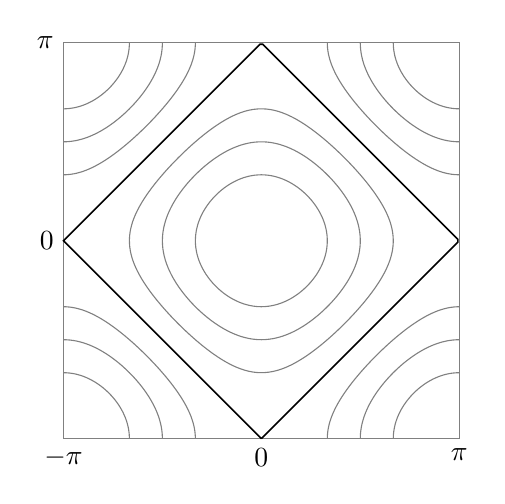
\begin{tikzpicture}[x=.8cm,y=.8cm]
\draw[gray] (-3.14159,-3.14159) rectangle (3.14159,3.14159);
\draw[gray] (2.0944,-3.1416) -- (2.0967,-3.0788) -- (2.1036,-3.0159) -- (2.1150,-2.9531) -- (2.1252,-2.9112) -- (2.1375,-2.8693) -- (2.1572,-2.8135) -- (2.1776,-2.7646) -- (2.1975,-2.7227) -- (2.2197,-2.6808) -- (2.2410,-2.6443) -- (2.2619,-2.6112) -- (2.2859,-2.5761) -- (2.3170,-2.5342) -- (2.3457,-2.4987) -- (2.3693,-2.4714) -- (2.4083,-2.4295) -- (2.4295,-2.4083) -- (2.4714,-2.3693) -- (2.4987,-2.3457) -- (2.5342,-2.3170) -- (2.5761,-2.2859) -- (2.6112,-2.2619) -- (2.6443,-2.2410) -- (2.6808,-2.2197) -- (2.7227,-2.1975) -- (2.7646,-2.1776) -- (2.8135,-2.1572) -- (2.8693,-2.1375) -- (2.9112,-2.1252) -- (2.9531,-2.1150) -- (3.0159,-2.1036) -- (3.0788,-2.0967) -- (3.1416,-2.0944) -- (3.1416,-2.0944);
\draw[gray] (-3.1416,-2.0944) -- (-3.0997,-2.0954) -- (-3.0369,-2.1008) -- (-2.9740,-2.1107) -- (-2.9322,-2.1198) -- (-2.8732,-2.1363) -- (-2.8274,-2.1519) -- (-2.7855,-2.1685) -- (-2.7437,-2.1873) -- (-2.7018,-2.2083) -- (-2.6599,-2.2317) -- (-2.6180,-2.2575) -- (-2.5804,-2.2829) -- (-2.5515,-2.3038) -- (-2.5133,-2.3337) -- (-2.4744,-2.3667) -- (-2.4504,-2.3884) -- (-2.4086,-2.4293) -- (-2.3876,-2.4513) -- (-2.3511,-2.4923) -- (-2.3248,-2.5244) -- (-2.3011,-2.5552) -- (-2.2714,-2.5970) -- (-2.2443,-2.6389) -- (-2.2201,-2.6801) -- (-2.1991,-2.7195) -- (-2.1782,-2.7633) -- (-2.1599,-2.8065) -- (-2.1445,-2.8484) -- (-2.1311,-2.8903) -- (-2.1153,-2.9515) -- (-2.1069,-2.9950) -- (-2.0985,-3.0578) -- (-2.0946,-3.1206) -- (-2.0944,-3.1416);
\draw[gray] (3.1416,2.0944) -- (3.0788,2.0967) -- (3.0159,2.1036) -- (2.9531,2.1150) -- (2.9112,2.1252) -- (2.8693,2.1375) -- (2.8135,2.1572) -- (2.7646,2.1776) -- (2.7227,2.1975) -- (2.6808,2.2197) -- (2.6443,2.2410) -- (2.6112,2.2619) -- (2.5761,2.2859) -- (2.5342,2.3170) -- (2.4987,2.3457) -- (2.4714,2.3693) -- (2.4295,2.4083) -- (2.4083,2.4295) -- (2.3693,2.4714) -- (2.3457,2.4987) -- (2.3170,2.5342) -- (2.2859,2.5761) -- (2.2619,2.6112) -- (2.2410,2.6443) -- (2.2197,2.6808) -- (2.1975,2.7227) -- (2.1776,2.7646) -- (2.1572,2.8135) -- (2.1375,2.8693) -- (2.1252,2.9112) -- (2.1150,2.9531) -- (2.1036,3.0159) -- (2.0967,3.0788) -- (2.0944,3.1416) -- (2.0944,3.1416);
\draw[gray] (-2.0944,3.1416) -- (-2.0954,3.0997) -- (-2.1008,3.0369) -- (-2.1107,2.9740) -- (-2.1198,2.9322) -- (-2.1363,2.8732) -- (-2.1519,2.8274) -- (-2.1685,2.7855) -- (-2.1873,2.7437) -- (-2.2083,2.7018) -- (-2.2317,2.6599) -- (-2.2575,2.6180) -- (-2.2829,2.5804) -- (-2.3038,2.5515) -- (-2.3337,2.5133) -- (-2.3667,2.4744) -- (-2.3884,2.4504) -- (-2.4293,2.4086) -- (-2.4513,2.3876) -- (-2.4923,2.3511) -- (-2.5244,2.3248) -- (-2.5552,2.3011) -- (-2.5970,2.2714) -- (-2.6389,2.2443) -- (-2.6801,2.2201) -- (-2.7195,2.1991) -- (-2.7633,2.1782) -- (-2.8065,2.1599) -- (-2.8484,2.1445) -- (-2.8903,2.1311) -- (-2.9515,2.1153) -- (-2.9950,2.1069) -- (-3.0578,2.0985) -- (-3.1206,2.0946) -- (-3.1416,2.0944);
\draw[gray] (1.5708,-3.1416) -- (1.5728,-3.0788) -- (1.5787,-3.0159) -- (1.5885,-2.9531) -- (1.5972,-2.9112) -- (1.6127,-2.8513) -- (1.6265,-2.8065) -- (1.6411,-2.7646) -- (1.6574,-2.7227) -- (1.6755,-2.6803) -- (1.6965,-2.6356) -- (1.7174,-2.5943) -- (1.7387,-2.5552) -- (1.7630,-2.5133) -- (1.7888,-2.4714) -- (1.8163,-2.4295) -- (1.8431,-2.3907) -- (1.8640,-2.3617) -- (1.8917,-2.3248) -- (1.9247,-2.2829) -- (1.9478,-2.2548) -- (1.9773,-2.2201) -- (2.0106,-2.1825) -- (2.0338,-2.1572) -- (2.0735,-2.1156) -- (2.0944,-2.0944) -- (2.1363,-2.0535) -- (2.1596,-2.0316) -- (2.1991,-1.9957) -- (2.2300,-1.9687) -- (2.2619,-1.9418) -- (2.3038,-1.9080) -- (2.3337,-1.8850) -- (2.3667,-1.8604) -- (2.4086,-1.8306) -- (2.4504,-1.8023) -- (2.4851,-1.7802) -- (2.5195,-1.7593) -- (2.5557,-1.7383) -- (2.5970,-1.7159) -- (2.6389,-1.6948) -- (2.6808,-1.6753) -- (2.7297,-1.6546) -- (2.7853,-1.6336) -- (2.8274,-1.6198) -- (2.8693,-1.6076) -- (2.9322,-1.5927) -- (2.9740,-1.5848) -- (3.0369,-1.5763) -- (3.0997,-1.5717) -- (3.1416,-1.5708) -- (3.1416,-1.5708);
\draw[gray] (-3.1416,-1.5708) -- (-3.0997,-1.5717) -- (-3.0369,-1.5763) -- (-2.9740,-1.5848) -- (-2.9322,-1.5927) -- (-2.8693,-1.6076) -- (-2.8274,-1.6198) -- (-2.7853,-1.6336) -- (-2.7297,-1.6546) -- (-2.6808,-1.6753) -- (-2.6389,-1.6948) -- (-2.5970,-1.7159) -- (-2.5557,-1.7383) -- (-2.5195,-1.7593) -- (-2.4851,-1.7802) -- (-2.4504,-1.8023) -- (-2.4086,-1.8306) -- (-2.3667,-1.8604) -- (-2.3337,-1.8850) -- (-2.3038,-1.9080) -- (-2.2619,-1.9418) -- (-2.2300,-1.9687) -- (-2.1991,-1.9957) -- (-2.1596,-2.0316) -- (-2.1363,-2.0535) -- (-2.0944,-2.0944) -- (-2.0735,-2.1156) -- (-2.0338,-2.1572) -- (-2.0106,-2.1825) -- (-1.9773,-2.2201) -- (-1.9478,-2.2548) -- (-1.9247,-2.2829) -- (-1.8917,-2.3248) -- (-1.8640,-2.3617) -- (-1.8431,-2.3907) -- (-1.8163,-2.4295) -- (-1.7888,-2.4714) -- (-1.7630,-2.5133) -- (-1.7387,-2.5552) -- (-1.7174,-2.5943) -- (-1.6965,-2.6356) -- (-1.6755,-2.6803) -- (-1.6574,-2.7227) -- (-1.6411,-2.7646) -- (-1.6265,-2.8065) -- (-1.6127,-2.8513) -- (-1.5972,-2.9112) -- (-1.5885,-2.9531) -- (-1.5787,-3.0159) -- (-1.5728,-3.0788) -- (-1.5708,-3.1416) -- (-1.5708,-3.1416);
\draw[gray] (3.1416,1.5708) -- (3.0788,1.5728) -- (3.0159,1.5787) -- (2.9531,1.5885) -- (2.9112,1.5972) -- (2.8513,1.6127) -- (2.8065,1.6265) -- (2.7646,1.6411) -- (2.7227,1.6574) -- (2.6803,1.6755) -- (2.6356,1.6965) -- (2.5943,1.7174) -- (2.5552,1.7387) -- (2.5133,1.7630) -- (2.4714,1.7888) -- (2.4295,1.8163) -- (2.3907,1.8431) -- (2.3617,1.8640) -- (2.3248,1.8917) -- (2.2829,1.9247) -- (2.2548,1.9478) -- (2.2201,1.9773) -- (2.1825,2.0106) -- (2.1572,2.0338) -- (2.1156,2.0735) -- (2.0944,2.0944) -- (2.0535,2.1363) -- (2.0316,2.1596) -- (1.9957,2.1991) -- (1.9687,2.2300) -- (1.9418,2.2619) -- (1.9080,2.3038) -- (1.8850,2.3337) -- (1.8604,2.3667) -- (1.8306,2.4086) -- (1.8023,2.4504) -- (1.7802,2.4851) -- (1.7593,2.5195) -- (1.7383,2.5557) -- (1.7159,2.5970) -- (1.6948,2.6389) -- (1.6753,2.6808) -- (1.6546,2.7297) -- (1.6336,2.7853) -- (1.6198,2.8274) -- (1.6076,2.8693) -- (1.5927,2.9322) -- (1.5848,2.9740) -- (1.5763,3.0369) -- (1.5717,3.0997) -- (1.5708,3.1416);
\draw[gray] (-1.5708,3.1416) -- (-1.5717,3.0997) -- (-1.5763,3.0369) -- (-1.5848,2.9740) -- (-1.5927,2.9322) -- (-1.6076,2.8693) -- (-1.6198,2.8274) -- (-1.6336,2.7853) -- (-1.6546,2.7297) -- (-1.6753,2.6808) -- (-1.6948,2.6389) -- (-1.7159,2.5970) -- (-1.7383,2.5557) -- (-1.7593,2.5195) -- (-1.7802,2.4851) -- (-1.8023,2.4504) -- (-1.8306,2.4086) -- (-1.8604,2.3667) -- (-1.8850,2.3337) -- (-1.9080,2.3038) -- (-1.9418,2.2619) -- (-1.9687,2.2300) -- (-1.9957,2.1991) -- (-2.0316,2.1596) -- (-2.0535,2.1363) -- (-2.0944,2.0944) -- (-2.1156,2.0735) -- (-2.1572,2.0338) -- (-2.1825,2.0106) -- (-2.2201,1.9773) -- (-2.2548,1.9478) -- (-2.2829,1.9247) -- (-2.3248,1.8917) -- (-2.3617,1.8640) -- (-2.3907,1.8431) -- (-2.4295,1.8163) -- (-2.4714,1.7888) -- (-2.5133,1.7630) -- (-2.5552,1.7387) -- (-2.5943,1.7174) -- (-2.6356,1.6965) -- (-2.6803,1.6755) -- (-2.7227,1.6574) -- (-2.7646,1.6411) -- (-2.8065,1.6265) -- (-2.8513,1.6127) -- (-2.9112,1.5972) -- (-2.9531,1.5885) -- (-3.0159,1.5787) -- (-3.0788,1.5728) -- (-3.1416,1.5708) -- (-3.1416,1.5708);
\draw[gray] (1.0472,-3.1416) -- (1.0495,-3.0788) -- (1.0562,-3.0159) -- (1.0675,-2.9531) -- (1.0774,-2.9112) -- (1.0892,-2.8693) -- (1.1100,-2.8073) -- (1.1265,-2.7646) -- (1.1444,-2.7227) -- (1.1639,-2.6808) -- (1.1850,-2.6389) -- (1.2075,-2.5970) -- (1.2314,-2.5552) -- (1.2566,-2.5133) -- (1.2776,-2.4801) -- (1.2985,-2.4480) -- (1.3252,-2.4086) -- (1.3546,-2.3667) -- (1.3823,-2.3287) -- (1.4032,-2.3007) -- (1.4329,-2.2619) -- (1.4660,-2.2201) -- (1.4870,-2.1941) -- (1.5174,-2.1572) -- (1.5499,-2.1188) -- (1.5708,-2.0944) -- (1.6075,-2.0525) -- (1.6336,-2.0233) -- (1.6642,-1.9897) -- (1.6965,-1.9549) -- (1.7228,-1.9268) -- (1.7593,-1.8888) -- (1.7834,-1.8640) -- (1.8221,-1.8248) -- (1.8459,-1.8012) -- (1.8850,-1.7630) -- (1.9105,-1.7383) -- (1.9478,-1.7031) -- (1.9774,-1.6755) -- (2.0106,-1.6451) -- (2.0467,-1.6127) -- (2.0735,-1.5890) -- (2.1153,-1.5528) -- (2.1435,-1.5289) -- (2.1782,-1.5000) -- (2.2200,-1.4661) -- (2.2464,-1.4451) -- (2.2829,-1.4168) -- (2.3248,-1.3852) -- (2.3574,-1.3614) -- (2.3876,-1.3398) -- (2.4295,-1.3109) -- (2.4714,-1.2831) -- (2.5133,-1.2566) -- (2.5479,-1.2357) -- (2.5842,-1.2147) -- (2.6223,-1.1938) -- (2.6628,-1.1729) -- (2.7064,-1.1519) -- (2.7540,-1.1310) -- (2.8065,-1.1103) -- (2.8484,-1.0958) -- (2.8903,-1.0831) -- (2.9504,-1.0681) -- (2.9950,-1.0595) -- (3.0578,-1.0512) -- (3.1206,-1.0474) -- (3.1416,-1.0472);
\draw[gray] (-3.1416,-1.0472) -- (-3.0997,-1.0482) -- (-3.0369,-1.0535) -- (-2.9740,-1.0633) -- (-2.9322,-1.0722) -- (-2.8698,-1.0891) -- (-2.8274,-1.1028) -- (-2.7855,-1.1182) -- (-2.7437,-1.1353) -- (-2.7018,-1.1540) -- (-2.6599,-1.1743) -- (-2.6180,-1.1961) -- (-2.5761,-1.2193) -- (-2.5342,-1.2438) -- (-2.4923,-1.2697) -- (-2.4504,-1.2969) -- (-2.4169,-1.3195) -- (-2.3867,-1.3404) -- (-2.3457,-1.3698) -- (-2.3038,-1.4008) -- (-2.2733,-1.4242) -- (-2.2410,-1.4493) -- (-2.1991,-1.4829) -- (-2.1686,-1.5080) -- (-2.1363,-1.5350) -- (-2.0944,-1.5708) -- (-2.0704,-1.5917) -- (-2.0316,-1.6262) -- (-2.0002,-1.6546) -- (-1.9687,-1.6835) -- (-1.9326,-1.7174) -- (-1.9059,-1.7428) -- (-1.8672,-1.7802) -- (-1.8431,-1.8040) -- (-1.8040,-1.8431) -- (-1.7802,-1.8672) -- (-1.7428,-1.9059) -- (-1.7174,-1.9326) -- (-1.6835,-1.9687) -- (-1.6546,-2.0002) -- (-1.6262,-2.0316) -- (-1.5917,-2.0704) -- (-1.5708,-2.0944) -- (-1.5350,-2.1363) -- (-1.5080,-2.1686) -- (-1.4829,-2.1991) -- (-1.4493,-2.2410) -- (-1.4242,-2.2733) -- (-1.4008,-2.3038) -- (-1.3698,-2.3457) -- (-1.3404,-2.3867) -- (-1.3195,-2.4169) -- (-1.2969,-2.4504) -- (-1.2697,-2.4923) -- (-1.2438,-2.5342) -- (-1.2193,-2.5761) -- (-1.1961,-2.6180) -- (-1.1743,-2.6599) -- (-1.1540,-2.7018) -- (-1.1353,-2.7437) -- (-1.1182,-2.7855) -- (-1.1028,-2.8274) -- (-1.0891,-2.8698) -- (-1.0722,-2.9322) -- (-1.0633,-2.9740) -- (-1.0535,-3.0369) -- (-1.0482,-3.0997) -- (-1.0472,-3.1416) -- (-1.0472,-3.1416);
\draw[gray] (3.1416,1.0472) -- (3.0788,1.0495) -- (3.0159,1.0562) -- (2.9531,1.0675) -- (2.9112,1.0774) -- (2.8693,1.0892) -- (2.8073,1.1100) -- (2.7646,1.1265) -- (2.7227,1.1444) -- (2.6808,1.1639) -- (2.6389,1.1850) -- (2.5970,1.2075) -- (2.5552,1.2314) -- (2.5133,1.2566) -- (2.4801,1.2776) -- (2.4480,1.2985) -- (2.4086,1.3252) -- (2.3667,1.3546) -- (2.3287,1.3823) -- (2.3007,1.4032) -- (2.2619,1.4329) -- (2.2201,1.4660) -- (2.1941,1.4870) -- (2.1572,1.5174) -- (2.1188,1.5499) -- (2.0944,1.5708) -- (2.0525,1.6075) -- (2.0233,1.6336) -- (1.9897,1.6642) -- (1.9549,1.6965) -- (1.9268,1.7228) -- (1.8888,1.7593) -- (1.8640,1.7834) -- (1.8248,1.8221) -- (1.8012,1.8459) -- (1.7630,1.8850) -- (1.7383,1.9105) -- (1.7031,1.9478) -- (1.6755,1.9774) -- (1.6451,2.0106) -- (1.6127,2.0467) -- (1.5890,2.0735) -- (1.5528,2.1153) -- (1.5289,2.1435) -- (1.5000,2.1782) -- (1.4661,2.2200) -- (1.4451,2.2464) -- (1.4168,2.2829) -- (1.3852,2.3248) -- (1.3614,2.3574) -- (1.3398,2.3876) -- (1.3109,2.4295) -- (1.2831,2.4714) -- (1.2566,2.5133) -- (1.2357,2.5479) -- (1.2147,2.5842) -- (1.1938,2.6223) -- (1.1729,2.6628) -- (1.1519,2.7064) -- (1.1310,2.7540) -- (1.1103,2.8065) -- (1.0958,2.8484) -- (1.0831,2.8903) -- (1.0681,2.9504) -- (1.0595,2.9950) -- (1.0512,3.0578) -- (1.0474,3.1206) -- (1.0472,3.1416);
\draw[gray] (-1.0472,3.1416) -- (-1.0482,3.0997) -- (-1.0535,3.0369) -- (-1.0633,2.9740) -- (-1.0722,2.9322) -- (-1.0891,2.8698) -- (-1.1028,2.8274) -- (-1.1182,2.7855) -- (-1.1353,2.7437) -- (-1.1540,2.7018) -- (-1.1743,2.6599) -- (-1.1961,2.6180) -- (-1.2193,2.5761) -- (-1.2438,2.5342) -- (-1.2697,2.4923) -- (-1.2969,2.4504) -- (-1.3195,2.4169) -- (-1.3404,2.3867) -- (-1.3698,2.3457) -- (-1.4008,2.3038) -- (-1.4242,2.2733) -- (-1.4493,2.2410) -- (-1.4829,2.1991) -- (-1.5080,2.1686) -- (-1.5350,2.1363) -- (-1.5708,2.0944) -- (-1.5917,2.0704) -- (-1.6262,2.0316) -- (-1.6546,2.0002) -- (-1.6835,1.9687) -- (-1.7174,1.9326) -- (-1.7428,1.9059) -- (-1.7802,1.8672) -- (-1.8040,1.8431) -- (-1.8431,1.8040) -- (-1.8672,1.7802) -- (-1.9059,1.7428) -- (-1.9326,1.7174) -- (-1.9687,1.6835) -- (-2.0002,1.6546) -- (-2.0316,1.6262) -- (-2.0704,1.5917) -- (-2.0944,1.5708) -- (-2.1363,1.5350) -- (-2.1686,1.5080) -- (-2.1991,1.4829) -- (-2.2410,1.4493) -- (-2.2733,1.4242) -- (-2.3038,1.4008) -- (-2.3457,1.3698) -- (-2.3867,1.3404) -- (-2.4169,1.3195) -- (-2.4504,1.2969) -- (-2.4923,1.2697) -- (-2.5342,1.2438) -- (-2.5761,1.2193) -- (-2.6180,1.1961) -- (-2.6599,1.1743) -- (-2.7018,1.1540) -- (-2.7437,1.1353) -- (-2.7855,1.1182) -- (-2.8274,1.1028) -- (-2.8698,1.0891) -- (-2.9322,1.0722) -- (-2.9740,1.0633) -- (-3.0369,1.0535) -- (-3.0997,1.0482) -- (-3.1416,1.0472);
\draw[black,semithick] (-0.0000,-3.1416) -- (0.0419,-3.0997) -- (0.0628,-3.0788) -- (0.1047,-3.0369) -- (0.1257,-3.0159) -- (0.1676,-2.9740) -- (0.1885,-2.9531) -- (0.2304,-2.9112) -- (0.2513,-2.8903) -- (0.2932,-2.8484) -- (0.3142,-2.8274) -- (0.3560,-2.7855) -- (0.3770,-2.7646) -- (0.4189,-2.7227) -- (0.4398,-2.7018) -- (0.4817,-2.6599) -- (0.5027,-2.6389) -- (0.5445,-2.5970) -- (0.5655,-2.5761) -- (0.6074,-2.5342) -- (0.6283,-2.5133) -- (0.6702,-2.4714) -- (0.6912,-2.4504) -- (0.7330,-2.4086) -- (0.7540,-2.3876) -- (0.7959,-2.3457) -- (0.8168,-2.3248) -- (0.8587,-2.2829) -- (0.8796,-2.2619) -- (0.9215,-2.2201) -- (0.9425,-2.1991) -- (0.9844,-2.1572) -- (1.0053,-2.1363) -- (1.0472,-2.0944) -- (1.0681,-2.0735) -- (1.1100,-2.0316) -- (1.1310,-2.0106) -- (1.1729,-1.9687) -- (1.1938,-1.9478) -- (1.2357,-1.9059) -- (1.2566,-1.8850) -- (1.2985,-1.8431) -- (1.3195,-1.8221) -- (1.3614,-1.7802) -- (1.3823,-1.7593) -- (1.4242,-1.7174) -- (1.4451,-1.6965) -- (1.4870,-1.6546) -- (1.5080,-1.6336) -- (1.5499,-1.5917) -- (1.5708,-1.5708) -- (1.6127,-1.5289) -- (1.6336,-1.5080) -- (1.6755,-1.4661) -- (1.6965,-1.4451) -- (1.7383,-1.4032) -- (1.7593,-1.3823) -- (1.8012,-1.3404) -- (1.8221,-1.3195) -- (1.8640,-1.2776) -- (1.8850,-1.2566) -- (1.9268,-1.2147) -- (1.9478,-1.1938) -- (1.9897,-1.1519) -- (2.0106,-1.1310) -- (2.0525,-1.0891) -- (2.0735,-1.0681) -- (2.1153,-1.0263) -- (2.1363,-1.0053) -- (2.1782,-0.9634) -- (2.1991,-0.9425) -- (2.2410,-0.9006) -- (2.2619,-0.8796) -- (2.3038,-0.8378) -- (2.3248,-0.8168) -- (2.3667,-0.7749) -- (2.3876,-0.7540) -- (2.4295,-0.7121) -- (2.4504,-0.6912) -- (2.4923,-0.6493) -- (2.5133,-0.6283) -- (2.5552,-0.5864) -- (2.5761,-0.5655) -- (2.6180,-0.5236) -- (2.6389,-0.5027) -- (2.6808,-0.4608) -- (2.7018,-0.4398) -- (2.7437,-0.3979) -- (2.7646,-0.3770) -- (2.8065,-0.3351) -- (2.8274,-0.3142) -- (2.8693,-0.2723) -- (2.8903,-0.2513) -- (2.9322,-0.2094) -- (2.9531,-0.1885) -- (2.9950,-0.1466) -- (3.0159,-0.1257) -- (3.0578,-0.0838) -- (3.0788,-0.0628) -- (3.1206,-0.0209) -- (3.1206,0.0209) -- (3.0997,0.0419) -- (3.0578,0.0838) -- (3.0369,0.1047) -- (2.9950,0.1466) -- (2.9740,0.1676) -- (2.9322,0.2094) -- (2.9112,0.2304) -- (2.8693,0.2723) -- (2.8484,0.2932) -- (2.8065,0.3351) -- (2.7855,0.3560) -- (2.7437,0.3979) -- (2.7227,0.4189) -- (2.6808,0.4608) -- (2.6599,0.4817) -- (2.6180,0.5236) -- (2.5970,0.5445) -- (2.5552,0.5864) -- (2.5342,0.6074) -- (2.4923,0.6493) -- (2.4714,0.6702) -- (2.4295,0.7121) -- (2.4086,0.7330) -- (2.3667,0.7749) -- (2.3457,0.7959) -- (2.3038,0.8378) -- (2.2829,0.8587) -- (2.2410,0.9006) -- (2.2201,0.9215) -- (2.1782,0.9634) -- (2.1572,0.9844) -- (2.1153,1.0263) -- (2.0944,1.0472) -- (2.0525,1.0891) -- (2.0316,1.1100) -- (1.9897,1.1519) -- (1.9687,1.1729) -- (1.9268,1.2147) -- (1.9059,1.2357) -- (1.8640,1.2776) -- (1.8431,1.2985) -- (1.8012,1.3404) -- (1.7802,1.3614) -- (1.7383,1.4032) -- (1.7174,1.4242) -- (1.6755,1.4661) -- (1.6546,1.4870) -- (1.6127,1.5289) -- (1.5917,1.5499) -- (1.5499,1.5917) -- (1.5289,1.6127) -- (1.4870,1.6546) -- (1.4661,1.6755) -- (1.4242,1.7174) -- (1.4032,1.7383) -- (1.3614,1.7802) -- (1.3404,1.8012) -- (1.2985,1.8431) -- (1.2776,1.8640) -- (1.2357,1.9059) -- (1.2147,1.9268) -- (1.1729,1.9687) -- (1.1519,1.9897) -- (1.1100,2.0316) -- (1.0891,2.0525) -- (1.0472,2.0944) -- (1.0263,2.1153) -- (0.9844,2.1572) -- (0.9634,2.1782) -- (0.9215,2.2201) -- (0.9006,2.2410) -- (0.8587,2.2829) -- (0.8378,2.3038) -- (0.7959,2.3457) -- (0.7749,2.3667) -- (0.7330,2.4086) -- (0.7121,2.4295) -- (0.6702,2.4714) -- (0.6493,2.4923) -- (0.6074,2.5342) -- (0.5864,2.5552) -- (0.5445,2.5970) -- (0.5236,2.6180) -- (0.4817,2.6599) -- (0.4608,2.6808) -- (0.4189,2.7227) -- (0.3979,2.7437) -- (0.3560,2.7855) -- (0.3351,2.8065) -- (0.2932,2.8484) -- (0.2723,2.8693) -- (0.2304,2.9112) -- (0.2094,2.9322) -- (0.1676,2.9740) -- (0.1466,2.9950) -- (0.1047,3.0369) -- (0.0838,3.0578) -- (0.0419,3.0997) -- (0.0209,3.1206) -- (-0.0209,3.1206) -- (-0.0628,3.0788) -- (-0.0838,3.0578) -- (-0.1257,3.0159) -- (-0.1466,2.9950) -- (-0.1885,2.9531) -- (-0.2094,2.9322) -- (-0.2513,2.8903) -- (-0.2723,2.8693) -- (-0.3142,2.8274) -- (-0.3351,2.8065) -- (-0.3770,2.7646) -- (-0.3979,2.7437) -- (-0.4398,2.7018) -- (-0.4608,2.6808) -- (-0.5027,2.6389) -- (-0.5236,2.6180) -- (-0.5655,2.5761) -- (-0.5864,2.5552) -- (-0.6283,2.5133) -- (-0.6493,2.4923) -- (-0.6912,2.4504) -- (-0.7121,2.4295) -- (-0.7540,2.3876) -- (-0.7749,2.3667) -- (-0.8168,2.3248) -- (-0.8378,2.3038) -- (-0.8796,2.2619) -- (-0.9006,2.2410) -- (-0.9425,2.1991) -- (-0.9634,2.1782) -- (-1.0053,2.1363) -- (-1.0263,2.1153) -- (-1.0681,2.0735) -- (-1.0891,2.0525) -- (-1.1310,2.0106) -- (-1.1519,1.9897) -- (-1.1938,1.9478) -- (-1.2147,1.9268) -- (-1.2566,1.8850) -- (-1.2776,1.8640) -- (-1.3195,1.8221) -- (-1.3404,1.8012) -- (-1.3823,1.7593) -- (-1.4032,1.7383) -- (-1.4451,1.6965) -- (-1.4661,1.6755) -- (-1.5080,1.6336) -- (-1.5289,1.6127) -- (-1.5708,1.5708) -- (-1.5917,1.5499) -- (-1.6336,1.5080) -- (-1.6546,1.4870) -- (-1.6965,1.4451) -- (-1.7174,1.4242) -- (-1.7593,1.3823) -- (-1.7802,1.3614) -- (-1.8221,1.3195) -- (-1.8431,1.2985) -- (-1.8850,1.2566) -- (-1.9059,1.2357) -- (-1.9478,1.1938) -- (-1.9687,1.1729) -- (-2.0106,1.1310) -- (-2.0316,1.1100) -- (-2.0735,1.0681) -- (-2.0944,1.0472) -- (-2.1363,1.0053) -- (-2.1572,0.9844) -- (-2.1991,0.9425) -- (-2.2201,0.9215) -- (-2.2619,0.8796) -- (-2.2829,0.8587) -- (-2.3248,0.8168) -- (-2.3457,0.7959) -- (-2.3876,0.7540) -- (-2.4086,0.7330) -- (-2.4504,0.6912) -- (-2.4714,0.6702) -- (-2.5133,0.6283) -- (-2.5342,0.6074) -- (-2.5761,0.5655) -- (-2.5970,0.5445) -- (-2.6389,0.5027) -- (-2.6599,0.4817) -- (-2.7018,0.4398) -- (-2.7227,0.4189) -- (-2.7646,0.3770) -- (-2.7855,0.3560) -- (-2.8274,0.3142) -- (-2.8484,0.2932) -- (-2.8903,0.2513) -- (-2.9112,0.2304) -- (-2.9531,0.1885) -- (-2.9740,0.1676) -- (-3.0159,0.1257) -- (-3.0369,0.1047) -- (-3.0788,0.0628) -- (-3.0997,0.0419) -- (-3.1416,-0.0000) -- (-3.0997,-0.0419) -- (-3.0788,-0.0628) -- (-3.0369,-0.1047) -- (-3.0159,-0.1257) -- (-2.9740,-0.1676) -- (-2.9531,-0.1885) -- (-2.9112,-0.2304) -- (-2.8903,-0.2513) -- (-2.8484,-0.2932) -- (-2.8274,-0.3142) -- (-2.7855,-0.3560) -- (-2.7646,-0.3770) -- (-2.7227,-0.4189) -- (-2.7018,-0.4398) -- (-2.6599,-0.4817) -- (-2.6389,-0.5027) -- (-2.5970,-0.5445) -- (-2.5761,-0.5655) -- (-2.5342,-0.6074) -- (-2.5133,-0.6283) -- (-2.4714,-0.6702) -- (-2.4504,-0.6912) -- (-2.4086,-0.7330) -- (-2.3876,-0.7540) -- (-2.3457,-0.7959) -- (-2.3248,-0.8168) -- (-2.2829,-0.8587) -- (-2.2619,-0.8796) -- (-2.2201,-0.9215) -- (-2.1991,-0.9425) -- (-2.1572,-0.9844) -- (-2.1363,-1.0053) -- (-2.0944,-1.0472) -- (-2.0735,-1.0681) -- (-2.0316,-1.1100) -- (-2.0106,-1.1310) -- (-1.9687,-1.1729) -- (-1.9478,-1.1938) -- (-1.9059,-1.2357) -- (-1.8850,-1.2566) -- (-1.8431,-1.2985) -- (-1.8221,-1.3195) -- (-1.7802,-1.3614) -- (-1.7593,-1.3823) -- (-1.7174,-1.4242) -- (-1.6965,-1.4451) -- (-1.6546,-1.4870) -- (-1.6336,-1.5080) -- (-1.5917,-1.5499) -- (-1.5708,-1.5708) -- (-1.5289,-1.6127) -- (-1.5080,-1.6336) -- (-1.4661,-1.6755) -- (-1.4451,-1.6965) -- (-1.4032,-1.7383) -- (-1.3823,-1.7593) -- (-1.3404,-1.8012) -- (-1.3195,-1.8221) -- (-1.2776,-1.8640) -- (-1.2566,-1.8850) -- (-1.2147,-1.9268) -- (-1.1938,-1.9478) -- (-1.1519,-1.9897) -- (-1.1310,-2.0106) -- (-1.0891,-2.0525) -- (-1.0681,-2.0735) -- (-1.0263,-2.1153) -- (-1.0053,-2.1363) -- (-0.9634,-2.1782) -- (-0.9425,-2.1991) -- (-0.9006,-2.2410) -- (-0.8796,-2.2619) -- (-0.8378,-2.3038) -- (-0.8168,-2.3248) -- (-0.7749,-2.3667) -- (-0.7540,-2.3876) -- (-0.7121,-2.4295) -- (-0.6912,-2.4504) -- (-0.6493,-2.4923) -- (-0.6283,-2.5133) -- (-0.5864,-2.5552) -- (-0.5655,-2.5761) -- (-0.5236,-2.6180) -- (-0.5027,-2.6389) -- (-0.4608,-2.6808) -- (-0.4398,-2.7018) -- (-0.3979,-2.7437) -- (-0.3770,-2.7646) -- (-0.3351,-2.8065) -- (-0.3142,-2.8274) -- (-0.2723,-2.8693) -- (-0.2513,-2.8903) -- (-0.2094,-2.9322) -- (-0.1885,-2.9531) -- (-0.1466,-2.9950) -- (-0.1257,-3.0159) -- (-0.0838,-3.0578) -- (-0.0628,-3.0788) -- (-0.0209,-3.1206) -- (-0.0000,-3.1416);
\draw[gray] (-0.1885,-2.0741) -- (-0.1257,-2.0853) -- (-0.0628,-2.0921) -- (-0.0000,-2.0944) -- (0.0628,-2.0921) -- (0.1257,-2.0853) -- (0.1885,-2.0741) -- (0.2304,-2.0642) -- (0.2723,-2.0524) -- (0.3343,-2.0316) -- (0.3770,-2.0151) -- (0.4189,-1.9972) -- (0.4608,-1.9777) -- (0.5027,-1.9566) -- (0.5445,-1.9341) -- (0.5864,-1.9102) -- (0.6283,-1.8850) -- (0.6615,-1.8640) -- (0.6936,-1.8431) -- (0.7330,-1.8164) -- (0.7749,-1.7870) -- (0.8129,-1.7593) -- (0.8409,-1.7383) -- (0.8796,-1.7087) -- (0.9215,-1.6756) -- (0.9475,-1.6546) -- (0.9844,-1.6242) -- (1.0228,-1.5917) -- (1.0472,-1.5708) -- (1.0891,-1.5341) -- (1.1183,-1.5080) -- (1.1519,-1.4774) -- (1.1867,-1.4451) -- (1.2147,-1.4188) -- (1.2528,-1.3823) -- (1.2776,-1.3582) -- (1.3168,-1.3195) -- (1.3404,-1.2957) -- (1.3786,-1.2566) -- (1.4032,-1.2311) -- (1.4385,-1.1938) -- (1.4661,-1.1642) -- (1.4965,-1.1310) -- (1.5289,-1.0949) -- (1.5525,-1.0681) -- (1.5888,-1.0263) -- (1.6127,-0.9981) -- (1.6416,-0.9634) -- (1.6755,-0.9216) -- (1.6965,-0.8952) -- (1.7248,-0.8587) -- (1.7564,-0.8168) -- (1.7802,-0.7842) -- (1.8018,-0.7540) -- (1.8307,-0.7121) -- (1.8585,-0.6702) -- (1.8850,-0.6283) -- (1.9059,-0.5936) -- (1.9268,-0.5574) -- (1.9478,-0.5193) -- (1.9687,-0.4788) -- (1.9897,-0.4352) -- (2.0106,-0.3876) -- (2.0313,-0.3351) -- (2.0458,-0.2932) -- (2.0585,-0.2513) -- (2.0735,-0.1912) -- (2.0821,-0.1466) -- (2.0904,-0.0838) -- (2.0941,-0.0209) -- (2.0944,0.0000) -- (2.0921,0.0628) -- (2.0853,0.1257) -- (2.0741,0.1885) -- (2.0642,0.2304) -- (2.0524,0.2723) -- (2.0316,0.3343) -- (2.0151,0.3770) -- (1.9972,0.4189) -- (1.9777,0.4608) -- (1.9566,0.5027) -- (1.9341,0.5445) -- (1.9102,0.5864) -- (1.8850,0.6283) -- (1.8640,0.6615) -- (1.8431,0.6936) -- (1.8164,0.7330) -- (1.7870,0.7749) -- (1.7593,0.8129) -- (1.7383,0.8409) -- (1.7087,0.8796) -- (1.6756,0.9215) -- (1.6546,0.9475) -- (1.6242,0.9844) -- (1.5917,1.0228) -- (1.5708,1.0472) -- (1.5341,1.0891) -- (1.5080,1.1183) -- (1.4774,1.1519) -- (1.4451,1.1867) -- (1.4188,1.2147) -- (1.3823,1.2528) -- (1.3582,1.2776) -- (1.3195,1.3168) -- (1.2957,1.3404) -- (1.2566,1.3786) -- (1.2311,1.4032) -- (1.1938,1.4385) -- (1.1642,1.4661) -- (1.1310,1.4965) -- (1.0949,1.5289) -- (1.0681,1.5525) -- (1.0263,1.5888) -- (0.9981,1.6127) -- (0.9634,1.6416) -- (0.9216,1.6755) -- (0.8952,1.6965) -- (0.8587,1.7248) -- (0.8168,1.7564) -- (0.7842,1.7802) -- (0.7540,1.8018) -- (0.7121,1.8307) -- (0.6702,1.8585) -- (0.6283,1.8850) -- (0.5936,1.9059) -- (0.5574,1.9268) -- (0.5193,1.9478) -- (0.4788,1.9687) -- (0.4352,1.9897) -- (0.3876,2.0106) -- (0.3351,2.0313) -- (0.2932,2.0458) -- (0.2513,2.0585) -- (0.1912,2.0735) -- (0.1466,2.0821) -- (0.0838,2.0904) -- (0.0209,2.0941) -- (-0.0000,2.0944) -- (-0.0628,2.0921) -- (-0.1257,2.0853) -- (-0.1885,2.0741) -- (-0.2304,2.0642) -- (-0.2723,2.0524) -- (-0.3343,2.0316) -- (-0.3770,2.0151) -- (-0.4189,1.9972) -- (-0.4608,1.9777) -- (-0.5027,1.9566) -- (-0.5445,1.9341) -- (-0.5864,1.9102) -- (-0.6283,1.8850) -- (-0.6615,1.8640) -- (-0.6936,1.8431) -- (-0.7330,1.8164) -- (-0.7749,1.7870) -- (-0.8129,1.7593) -- (-0.8409,1.7383) -- (-0.8796,1.7087) -- (-0.9215,1.6756) -- (-0.9475,1.6546) -- (-0.9844,1.6242) -- (-1.0228,1.5917) -- (-1.0472,1.5708) -- (-1.0891,1.5341) -- (-1.1183,1.5080) -- (-1.1519,1.4774) -- (-1.1867,1.4451) -- (-1.2147,1.4188) -- (-1.2528,1.3823) -- (-1.2776,1.3582) -- (-1.3168,1.3195) -- (-1.3404,1.2957) -- (-1.3786,1.2566) -- (-1.4032,1.2311) -- (-1.4385,1.1938) -- (-1.4661,1.1642) -- (-1.4965,1.1310) -- (-1.5289,1.0949) -- (-1.5525,1.0681) -- (-1.5888,1.0263) -- (-1.6127,0.9981) -- (-1.6416,0.9634) -- (-1.6755,0.9216) -- (-1.6965,0.8952) -- (-1.7248,0.8587) -- (-1.7564,0.8168) -- (-1.7802,0.7842) -- (-1.8018,0.7540) -- (-1.8307,0.7121) -- (-1.8585,0.6702) -- (-1.8850,0.6283) -- (-1.9059,0.5936) -- (-1.9268,0.5574) -- (-1.9478,0.5193) -- (-1.9687,0.4788) -- (-1.9897,0.4352) -- (-2.0106,0.3876) -- (-2.0313,0.3351) -- (-2.0458,0.2932) -- (-2.0585,0.2513) -- (-2.0735,0.1912) -- (-2.0821,0.1466) -- (-2.0904,0.0838) -- (-2.0941,0.0209) -- (-2.0934,-0.0419) -- (-2.0881,-0.1047) -- (-2.0783,-0.1676) -- (-2.0694,-0.2094) -- (-2.0525,-0.2718) -- (-2.0388,-0.3142) -- (-2.0234,-0.3560) -- (-2.0063,-0.3979) -- (-1.9876,-0.4398) -- (-1.9673,-0.4817) -- (-1.9455,-0.5236) -- (-1.9223,-0.5655) -- (-1.8978,-0.6074) -- (-1.8719,-0.6493) -- (-1.8447,-0.6912) -- (-1.8221,-0.7247) -- (-1.8012,-0.7549) -- (-1.7718,-0.7959) -- (-1.7407,-0.8378) -- (-1.7174,-0.8683) -- (-1.6922,-0.9006) -- (-1.6587,-0.9425) -- (-1.6336,-0.9730) -- (-1.6066,-1.0053) -- (-1.5708,-1.0472) -- (-1.5499,-1.0712) -- (-1.5154,-1.1100) -- (-1.4870,-1.1414) -- (-1.4581,-1.1729) -- (-1.4242,-1.2090) -- (-1.3988,-1.2357) -- (-1.3614,-1.2744) -- (-1.3376,-1.2985) -- (-1.2985,-1.3376) -- (-1.2744,-1.3614) -- (-1.2357,-1.3988) -- (-1.2090,-1.4242) -- (-1.1729,-1.4581) -- (-1.1414,-1.4870) -- (-1.1100,-1.5154) -- (-1.0712,-1.5499) -- (-1.0472,-1.5708) -- (-1.0053,-1.6066) -- (-0.9730,-1.6336) -- (-0.9425,-1.6587) -- (-0.9006,-1.6922) -- (-0.8683,-1.7174) -- (-0.8378,-1.7407) -- (-0.7959,-1.7718) -- (-0.7549,-1.8012) -- (-0.7247,-1.8221) -- (-0.6912,-1.8447) -- (-0.6493,-1.8719) -- (-0.6074,-1.8978) -- (-0.5655,-1.9223) -- (-0.5236,-1.9455) -- (-0.4817,-1.9673) -- (-0.4398,-1.9876) -- (-0.3979,-2.0063) -- (-0.3560,-2.0234) -- (-0.3142,-2.0388) -- (-0.2718,-2.0525) -- (-0.2094,-2.0694) -- (-0.1885,-2.0741);
\draw[gray] (-0.1885,-1.5531) -- (-0.1257,-1.5629) -- (-0.0628,-1.5688) -- (-0.0000,-1.5708) -- (0.0628,-1.5688) -- (0.1257,-1.5629) -- (0.1885,-1.5531) -- (0.2304,-1.5444) -- (0.2903,-1.5289) -- (0.3351,-1.5151) -- (0.3770,-1.5005) -- (0.4189,-1.4842) -- (0.4613,-1.4661) -- (0.5060,-1.4451) -- (0.5473,-1.4242) -- (0.5864,-1.4029) -- (0.6283,-1.3786) -- (0.6702,-1.3528) -- (0.7121,-1.3253) -- (0.7509,-1.2985) -- (0.7799,-1.2776) -- (0.8168,-1.2498) -- (0.8587,-1.2169) -- (0.8868,-1.1938) -- (0.9215,-1.1643) -- (0.9591,-1.1310) -- (0.9844,-1.1078) -- (1.0260,-1.0681) -- (1.0472,-1.0472) -- (1.0881,-1.0053) -- (1.1100,-0.9820) -- (1.1459,-0.9425) -- (1.1729,-0.9116) -- (1.1997,-0.8796) -- (1.2336,-0.8378) -- (1.2566,-0.8079) -- (1.2812,-0.7749) -- (1.3110,-0.7330) -- (1.3392,-0.6912) -- (1.3614,-0.6565) -- (1.3823,-0.6221) -- (1.4032,-0.5859) -- (1.4256,-0.5445) -- (1.4468,-0.5027) -- (1.4663,-0.4608) -- (1.4870,-0.4119) -- (1.5080,-0.3562) -- (1.5218,-0.3142) -- (1.5339,-0.2723) -- (1.5489,-0.2094) -- (1.5568,-0.1676) -- (1.5653,-0.1047) -- (1.5699,-0.0419) -- (1.5706,0.0209) -- (1.5673,0.0838) -- (1.5601,0.1466) -- (1.5499,0.2048) -- (1.5394,0.2513) -- (1.5281,0.2932) -- (1.5080,0.3560) -- (1.4926,0.3979) -- (1.4755,0.4398) -- (1.4567,0.4817) -- (1.4364,0.5236) -- (1.4145,0.5655) -- (1.3910,0.6074) -- (1.3659,0.6493) -- (1.3404,0.6893) -- (1.3195,0.7207) -- (1.2963,0.7540) -- (1.2657,0.7959) -- (1.2357,0.8350) -- (1.2147,0.8613) -- (1.1822,0.9006) -- (1.1519,0.9357) -- (1.1271,0.9634) -- (1.0891,1.0043) -- (1.0679,1.0263) -- (1.0263,1.0679) -- (1.0043,1.0891) -- (0.9634,1.1271) -- (0.9357,1.1519) -- (0.9006,1.1822) -- (0.8613,1.2147) -- (0.8350,1.2357) -- (0.7959,1.2657) -- (0.7540,1.2963) -- (0.7207,1.3195) -- (0.6893,1.3404) -- (0.6493,1.3659) -- (0.6074,1.3910) -- (0.5655,1.4145) -- (0.5236,1.4364) -- (0.4817,1.4567) -- (0.4398,1.4755) -- (0.3979,1.4926) -- (0.3560,1.5080) -- (0.2932,1.5281) -- (0.2513,1.5394) -- (0.2048,1.5499) -- (0.1466,1.5601) -- (0.0838,1.5673) -- (0.0209,1.5706) -- (-0.0419,1.5699) -- (-0.1047,1.5653) -- (-0.1676,1.5568) -- (-0.2094,1.5489) -- (-0.2723,1.5339) -- (-0.3142,1.5218) -- (-0.3562,1.5080) -- (-0.4119,1.4870) -- (-0.4608,1.4663) -- (-0.5027,1.4468) -- (-0.5445,1.4256) -- (-0.5859,1.4032) -- (-0.6221,1.3823) -- (-0.6565,1.3614) -- (-0.6912,1.3392) -- (-0.7330,1.3110) -- (-0.7749,1.2812) -- (-0.8079,1.2566) -- (-0.8378,1.2336) -- (-0.8796,1.1997) -- (-0.9116,1.1729) -- (-0.9425,1.1459) -- (-0.9820,1.1100) -- (-1.0053,1.0881) -- (-1.0472,1.0472) -- (-1.0681,1.0260) -- (-1.1078,0.9844) -- (-1.1310,0.9591) -- (-1.1643,0.9215) -- (-1.1938,0.8868) -- (-1.2169,0.8587) -- (-1.2498,0.8168) -- (-1.2776,0.7799) -- (-1.2985,0.7509) -- (-1.3253,0.7121) -- (-1.3528,0.6702) -- (-1.3786,0.6283) -- (-1.4029,0.5864) -- (-1.4242,0.5473) -- (-1.4451,0.5060) -- (-1.4661,0.4613) -- (-1.4842,0.4189) -- (-1.5005,0.3770) -- (-1.5151,0.3351) -- (-1.5289,0.2903) -- (-1.5444,0.2304) -- (-1.5531,0.1885) -- (-1.5629,0.1257) -- (-1.5688,0.0628) -- (-1.5708,-0.0000) -- (-1.5688,-0.0628) -- (-1.5629,-0.1257) -- (-1.5531,-0.1885) -- (-1.5444,-0.2304) -- (-1.5289,-0.2903) -- (-1.5151,-0.3351) -- (-1.5005,-0.3770) -- (-1.4842,-0.4189) -- (-1.4661,-0.4613) -- (-1.4451,-0.5060) -- (-1.4242,-0.5473) -- (-1.4029,-0.5864) -- (-1.3786,-0.6283) -- (-1.3528,-0.6702) -- (-1.3253,-0.7121) -- (-1.2985,-0.7509) -- (-1.2776,-0.7799) -- (-1.2498,-0.8168) -- (-1.2169,-0.8587) -- (-1.1938,-0.8868) -- (-1.1643,-0.9215) -- (-1.1310,-0.9591) -- (-1.1078,-0.9844) -- (-1.0681,-1.0260) -- (-1.0472,-1.0472) -- (-1.0053,-1.0881) -- (-0.9820,-1.1100) -- (-0.9425,-1.1459) -- (-0.9116,-1.1729) -- (-0.8796,-1.1997) -- (-0.8378,-1.2336) -- (-0.8079,-1.2566) -- (-0.7749,-1.2812) -- (-0.7330,-1.3110) -- (-0.6912,-1.3392) -- (-0.6565,-1.3614) -- (-0.6221,-1.3823) -- (-0.5859,-1.4032) -- (-0.5445,-1.4256) -- (-0.5027,-1.4468) -- (-0.4608,-1.4663) -- (-0.4119,-1.4870) -- (-0.3562,-1.5080) -- (-0.3142,-1.5218) -- (-0.2723,-1.5339) -- (-0.2094,-1.5489) -- (-0.1885,-1.5531);
\draw[gray] (-0.1885,-1.0266) -- (-0.1257,-1.0380) -- (-0.0628,-1.0449) -- (-0.0000,-1.0472) -- (0.0628,-1.0449) -- (0.1257,-1.0380) -- (0.1885,-1.0266) -- (0.2304,-1.0164) -- (0.2723,-1.0041) -- (0.3281,-0.9844) -- (0.3770,-0.9640) -- (0.4189,-0.9441) -- (0.4608,-0.9219) -- (0.4973,-0.9006) -- (0.5304,-0.8796) -- (0.5655,-0.8557) -- (0.6074,-0.8246) -- (0.6429,-0.7959) -- (0.6702,-0.7723) -- (0.7121,-0.7332) -- (0.7332,-0.7121) -- (0.7723,-0.6702) -- (0.7959,-0.6429) -- (0.8246,-0.6074) -- (0.8557,-0.5655) -- (0.8796,-0.5304) -- (0.9006,-0.4973) -- (0.9219,-0.4608) -- (0.9441,-0.4189) -- (0.9640,-0.3770) -- (0.9844,-0.3281) -- (1.0041,-0.2723) -- (1.0164,-0.2304) -- (1.0266,-0.1885) -- (1.0380,-0.1257) -- (1.0449,-0.0628) -- (1.0472,-0.0000) -- (1.0469,0.0209) -- (1.0431,0.0838) -- (1.0347,0.1466) -- (1.0263,0.1901) -- (1.0105,0.2513) -- (0.9971,0.2932) -- (0.9817,0.3351) -- (0.9634,0.3783) -- (0.9425,0.4221) -- (0.9215,0.4615) -- (0.8973,0.5027) -- (0.8702,0.5445) -- (0.8405,0.5864) -- (0.8168,0.6172) -- (0.7905,0.6493) -- (0.7540,0.6903) -- (0.7330,0.7123) -- (0.6912,0.7532) -- (0.6672,0.7749) -- (0.6283,0.8079) -- (0.5901,0.8378) -- (0.5612,0.8587) -- (0.5236,0.8841) -- (0.4817,0.9099) -- (0.4398,0.9333) -- (0.3979,0.9543) -- (0.3560,0.9731) -- (0.3142,0.9897) -- (0.2684,1.0053) -- (0.2094,1.0218) -- (0.1676,1.0309) -- (0.1047,1.0408) -- (0.0419,1.0462) -- (-0.0000,1.0472) -- (-0.0419,1.0462) -- (-0.1047,1.0408) -- (-0.1676,1.0309) -- (-0.2094,1.0218) -- (-0.2684,1.0053) -- (-0.3142,0.9897) -- (-0.3560,0.9731) -- (-0.3979,0.9543) -- (-0.4398,0.9333) -- (-0.4817,0.9099) -- (-0.5236,0.8841) -- (-0.5612,0.8587) -- (-0.5901,0.8378) -- (-0.6283,0.8079) -- (-0.6672,0.7749) -- (-0.6912,0.7532) -- (-0.7330,0.7123) -- (-0.7540,0.6903) -- (-0.7905,0.6493) -- (-0.8168,0.6172) -- (-0.8405,0.5864) -- (-0.8702,0.5445) -- (-0.8973,0.5027) -- (-0.9215,0.4615) -- (-0.9425,0.4221) -- (-0.9634,0.3783) -- (-0.9817,0.3351) -- (-0.9971,0.2932) -- (-1.0105,0.2513) -- (-1.0263,0.1901) -- (-1.0347,0.1466) -- (-1.0431,0.0838) -- (-1.0469,0.0209) -- (-1.0462,-0.0419) -- (-1.0408,-0.1047) -- (-1.0309,-0.1676) -- (-1.0218,-0.2094) -- (-1.0053,-0.2684) -- (-0.9897,-0.3142) -- (-0.9731,-0.3560) -- (-0.9543,-0.3979) -- (-0.9333,-0.4398) -- (-0.9099,-0.4817) -- (-0.8841,-0.5236) -- (-0.8587,-0.5612) -- (-0.8378,-0.5901) -- (-0.8079,-0.6283) -- (-0.7749,-0.6672) -- (-0.7532,-0.6912) -- (-0.7123,-0.7330) -- (-0.6903,-0.7540) -- (-0.6493,-0.7905) -- (-0.6172,-0.8168) -- (-0.5864,-0.8405) -- (-0.5445,-0.8702) -- (-0.5027,-0.8973) -- (-0.4615,-0.9215) -- (-0.4221,-0.9425) -- (-0.3783,-0.9634) -- (-0.3351,-0.9817) -- (-0.2932,-0.9971) -- (-0.2513,-1.0105) -- (-0.1901,-1.0263) -- (-0.1885,-1.0266);
\node[below] at (-3.14159,-3.14159) {$-\pi$};
\node[below] at (0,-3.14159) {$0$};
\node[below] at (3.14159,-3.14159) {$\pi$};
\node[left] at (-3.14159,3.14159) {$\pi$};
\node[left] at (-3.14159,0) {$0$};
\end{tikzpicture}
\caption{Level sets of $\Psi(x,y)=\cos x+\cos y$. The separatrix $\Psi=0$ is drawn in black.}
\label{fig:stream-function}
\end{figure}

\subsection{Main ideas of the proof}
Suppose
\[
 L\omega=i\lambda\omega,\qquad
 \lambda\in\R\setminus\{0\},\qquad
 \psi=\Delta^{-1}\omega.
\]
The reflections across the two diagonal components of the
separatrix commute with $L_0$ and $\Delta$, and decompose the
problem into four parity classes; see \eqref{ee:reflections}.
Consider first the class even under both reflections.
Then $\psi$ satisfies a Neumann condition on the regular
edges of the positive cell $\mathcal C=\{\Psi>0\}$.

The algebra of the dipole permits the choice
$W=(\Psi-2)\nabla\Psi/|\nabla\Psi|^2$.
Its commutator with $L_0$ has the special form
$[L_0,W\cdot\nabla]=(\operatorname{div}W-1)L_0$.
This identity cancels the zeroth-order term in the virial
calculation and leaves an interior density $\mathcal J$
which is nonnegative, with a positive definite gradient
part at every regular interior point.
The remaining question is the sign of the separatrix flux.

Here the transport equation along the separatrix is essential.
To display the argument in its simplest form, suppose also
that $\psi$ vanishes at the saddle points.
On each directed separatrix arc $\gamma$, let $s\in\R$
be flow time and set $\xi=\tanh s\in(-1,1)$.
The canonical boundary unknown $F$ is determined by
\[
 \psi(\gamma(s))
 =-i(1-\xi^2)F'(\xi)-\lambda F(\xi),
 \qquad F(-1)=F(1)=0.
\]
The transport equation rewrites the boundary contribution
in terms of a quadratic form $\mathcal F_\lambda$.
The key identity is
\[
 \mathcal F_\lambda(F)
 =\frac12\int_{-1}^{1}
 \left|(1-\xi^2)F''-\xi F'+F-i\lambda F'\right|^2\,d\xi
 +\frac12\int_{-1}^{1}|F'|^2\,d\xi
 \ge0;
\]
see \eqref{ee:trace-sos}.
Consequently, the virial identity gives
\[
 0\le\int_{\mathcal C}\mathcal J
 =-2\sum_\gamma\mathcal F_\lambda(F_\gamma)\le0.
\]
It follows that $\nabla\psi=0$ in the cell, and symmetry
and the mean-zero normalization imply $\psi=\omega=0$.
The spectral parameter enters inside the boundary square,
so the argument applies to every nonzero $\lambda$.
The additional assumption at the saddles is removed by
subtracting the affine function matching the endpoint
values; the symmetry decomposition makes the remaining
endpoint contribution nonnegative.

The other parity classes need a further
argument. Odd reflection imposes a Dirichlet condition,
which leaves a positive normal-derivative term in the
boundary flux. Thus the preceding sign contradiction no
longer follows directly. We factor out the boundary
vanishing of $\psi$ and derive weighted virial identities
for the resulting quotients. In the mixed classes,
the contributions from adjacent edges must also be
combined before taking the limit at a saddle.

These reductions lead to explicit elliptic quadratic
forms with positive gradient terms but potentially
negative lower-order terms. To prove coercivity, we
construct positive comparison functions. Dividing by
such a function and integrating by parts separates a
nonnegative gradient square from a residual coefficient.
Bounds for this residual, together with the appropriate
weighted Poincare inequalities and boundary identities,
recover the required sign contradiction; see
Theorem~\ref{r4:dd-exclusion} and
\eqref{eq:mixed-static-coercivity}.

In this last step, exact arithmetic verifies the
coefficient inequalities for the explicit comparison
functions. After clearing positive denominators and
using rational bounds for logarithms, these become
polynomial inequalities on bounded regions.
Subdivision and nonnegative Bernstein coefficients
certify the inequalities throughout each region.
Thus the calculations establish a uniform coercive
bound, rather than checking the eigenvalue equation
at selected spectral parameters.

\subsection{Organization}
Section~\ref{sec:spectral-foundations} sets up the eigenvalue problem
and reduces it to four sectors, according to the parity under the two
reflections across the separatrix. Section~\ref{sec:ee-exclusion}
excludes eigenvalues in the even--even sector.
Section~\ref{sec:saddle-gains} establishes the regularity near the
separatrix needed to justify the boundary limits in the remaining
sectors. Section~\ref{sec:dd-exclusion} treats the odd--odd sector,
culminating in Theorem~\ref{r4:dd-exclusion}. The two mixed sectors
are treated in Sections~\ref{sec:mixed-regularity}
and~\ref{sec:mixed-exclusion}: the first derives the paired boundary
flux and the regularity of eigenfunctions, and the second constructs
the positive comparison functions that lead to the coercivity estimate
\eqref{eq:mixed-static-coercivity}. Section~\ref{sec:spectral-exclusion}
combines the sector results into the proof of Theorem~\ref{Intm6}.
Throughout the paper, $A\lesssim B$ means $A\le CB$, where $C$
depends only on fixed parameters; dependence on an additional
parameter is indicated by a subscript.

\section{Reflection sectors and domain}\label{sec:spectral-foundations}
On $\mathbb T^2=(\mathbb R/2\pi\mathbb Z)^2$, let
\[
 \Psi=\cos x+\cos y,\qquad
 L_0=\sin y\,\partial_x-\sin x\,\partial_y,\qquad
 H=-iL_0,\qquad A=I+\Delta^{-1}.
\]
The inverse Laplacian acts on mean-zero functions. Inner products are
linear in the first argument. We consider
\begin{equation}\label{sf:eigen}
 H(\omega+\psi)=\lambda\omega,\qquad
 \omega\in L^2_0(\mathbb T^2),\quad \psi=\Delta^{-1}\omega\in H^2,
 \qquad \lambda\in\mathbb R\setminus\{0\}.
\end{equation}
The transport equation is understood in distributions; it implies
$L_0\omega\in L^2$. Since $A\ge0$, pairing the equation with
$A\omega$ shows that $\lambda\langle A\omega,\omega\rangle$ is real.
If this quadratic form vanishes, then $A\omega=0$ and
$\omega=0$. Thus every nonzero eigenfunction has real $\lambda$.
Throughout, eigenfunctions are taken in the original $L^2$ domain
$\mathcal D$ of \eqref{Intm3}; no further regularity of $\omega$ is
assumed.

The reflections
\begin{equation}\label{ee:reflections}
 S_1(x,y)=(\pi-y,\pi-x),\qquad
 S_2(x,y)=(\pi+y,\pi+x)\pmod {2\pi}
\end{equation}
commute with $L_0$ and $\Delta$. Thus their four joint parity spaces
reduce the eigenvalue problem into even--even, odd--odd, and mixed
sectors. We also call the odd--odd sector DD, referring to its
Dirichlet realization on the positive cell, where we set $s=\Psi$.
The quarter rotation $R(x,y)=(y,-x)$ satisfies $R^2=S_1S_2$.

We retain the four first Laplace modes in $\ker A$; since
$\lambda\ne0$, the zero modes of $L$ do not enter the argument. Write
$Y=(\ker L_0)^\perp$. Every eigenfunction in \eqref{sf:eigen} belongs
to $Y$, since $H(\omega+\psi)$ is orthogonal to $\ker L_0$.

\section{The even--even sector}
\label{sec:ee-exclusion}

The fixed sets of $S_1,S_2$ are the two components of the
separatrix. Each reflection exchanges the positive and negative cells.

\begin{theorem}\label{ee:theorem}
Suppose $\omega\in L^2_0(\mathbb T^2)$, $\psi=\Delta^{-1}\omega$, and
\begin{equation}\label{ee:eigen}
 H(\omega+\psi)=\lambda\omega,
 \qquad \lambda\in\mathbb R\setminus\{0\},
\end{equation}
in the transport graph domain. If
\[
 \omega\circ S_1=\omega,\qquad \omega\circ S_2=\omega,
\]
then $\omega=0$. Thus the linearized dipole operator has no nonzero
imaginary eigenvalue in the sector even under both reflections
\eqref{ee:reflections}.
\end{theorem}

We use $\psi\in H^2$, with no assumption that $\omega\in H^1$.
Vorticity is restricted to almost every regular orbit; along a
sequence approaching the separatrix, these restrictions have a
canonical transport limit.

\subsection{A localized virial identity}

We begin with a virial identity for bounded vector fields.

\begin{lemma}\label{ee:bounded-virial}
Let $W$ be a real periodic vector field in $W^{3,\infty}$ and let
$f\in W^{2,\infty}$ be real. Suppose
\[
 [L_0,W\cdot\nabla]=fL_0.
\]
Every eigenfunction \eqref{ee:eigen} satisfies
\begin{equation}\label{ee:bounded-form}
 0=\int_{\mathbb T^2} f|\Delta\psi|^2
   +\int_{\mathbb T^2}(2\operatorname{sym}DW-fI)
                  \nabla\psi\cdot\overline{\nabla\psi}
   +\frac12\int_{\mathbb T^2}\Delta(f-\operatorname{div}W)|\psi|^2.
\end{equation}
All three integrals are defined for $\psi\in H^2$.
\end{lemma}

\begin{proof}
Put $A=I+\Delta^{-1}$, $a=A\omega$, $d=\operatorname{div}W$, and
$D=W\cdot\nabla+d/2$. Extend $\Delta^{-1}$ by zero on constants
and $A$ to $L^2$, since the following group need not preserve
mean zero. If $\Phi_t$ is the complete flow of $W$, then
\[
 U_t u=\operatorname{Jac}(\Phi_t)^{1/2}\,u\circ\Phi_t
\]
is a strongly continuous unitary group with generator $D$.
Taking divergence of the assumed commutator gives $L_0d=L_0f$.
Moreover
\[
 D\Phi_t(x)L_0(x)=c_t(x)L_0(\Phi_t(x)),\qquad
 c_t(x)=\exp\!\left(\int_0^t f(\Phi_\tau(x))\,d\tau\right),
\]
and $L_0\log\operatorname{Jac}(\Phi_t)=L_0\log c_t$. Consequently
\[
 HU_t=c_tU_tH-\frac i2(L_0\log c_t)U_t.
\]
This identity, first established on smooth functions and then closed
in the graph norm of $H$, shows that $U_t$ preserves $\mathcal D(H)$
and that
\[
 \frac{[H,U_t]}t\longrightarrow
 [H,D]=\frac12(fH+Hf)
\]
strongly from that graph domain to $L^2$.

The commutator $[D,A]=[D,\Delta^{-1}]$ is bounded on $L^2$:
$D\Delta^{-1}$ maps $L^2$ to $H^1$, while
$\Delta^{-1}D$ has the same mapping property when
$D:L^2\to H^{-1}$ is interpreted distributionally. Also $A$
preserves $\mathcal D(D)$, since $\Delta^{-1}$ maps $L^2$ into
$H^2\subset\mathcal D(D)$. The group commutator formula therefore
gives
\[
 \frac{[U_t,A]}t\longrightarrow[D,A]
 \quad\hbox{strongly on }L^2.
\]
Self-adjointness of $H,A$ and $Ha=\lambda\omega$ imply the exact
finite-difference identity
\[
 \langle[H,U_t]a,a\rangle
   =\lambda\langle[U_t,A]\omega,\omega\rangle.
\]
Passing to the limit and taking real parts yields
\begin{equation}\label{ee:commutator-limit}
 \operatorname{Re}\langle f\omega,\omega+\psi\rangle
   =\langle[D,A]\omega,\omega\rangle
   =2\operatorname{Re}\langle D\psi,\omega\rangle.
\end{equation}
The last equality follows by distributional integration by parts.
Approximation of $\psi$ in
$H^2$ justifies
\begin{align*}
 \operatorname{Re}\int f\Delta\psi\,\overline\psi
   &=-\int f|\nabla\psi|^2+\frac12\int\Delta f|\psi|^2,\\
 2\operatorname{Re}\int D\psi\,\overline{\Delta\psi}
   &=-2\int\operatorname{sym}DW\nabla\psi\cdot\overline{\nabla\psi}
       +\frac12\int\Delta d|\psi|^2.
\end{align*}
Substitution in \eqref{ee:commutator-limit} proves the assertion.
\end{proof}

On the positive cell $\mathcal C=\{\Psi>0\}$, use the level coordinate
\[
 r=\Psi,\qquad \rho=|\nabla\Psi|,
 \qquad \delta=\cos x-\cos y.
\]
Away from its elliptic center define the normal field
\begin{equation}\label{ee:normal-field}
 W=(r-2)\frac{\nabla r}{\rho^2},\qquad
 f=\frac{r(2-r)\delta^2}{\rho^4},\qquad
 c=\frac{r(2-r)}{\rho^2}.
\end{equation}
Direct differentiation gives
\begin{equation}\label{ee:normal-algebra}
 [L_0,W\cdot\nabla]=fL_0,\qquad
 \operatorname{div}W=f+1,\qquad
 2\operatorname{sym}DW-fI=\begin{pmatrix}2-c&0\\0&c\end{pmatrix}
\end{equation}
in the orthonormal normal--tangent frame of a regular level.
For example,
\[
 \operatorname{div}\frac{\nabla r}{\rho^2}
   =-\frac{r\delta^2}{\rho^4};
\]
the two diagonal entries in \eqref{ee:normal-algebra} then follow
from $\Delta r=-r$. Furthermore
\begin{equation}\label{ee:c-positive}
 \rho^2-r(2-r)=2(1-\cos x)(1-\cos y)\ge0,
 \qquad 0<c\le1\quad(0<r<2).
\end{equation}
Thus the density
\begin{equation}\label{ee:positive-density}
 \mathcal J=f|\omega|^2+(2-c)|\psi_n|^2+c|\psi_t|^2
\end{equation}
is nonnegative, and its gradient part is strictly positive on every
regular interior point unless $\nabla\psi=0$.

To check the hypotheses of Lemma~\ref{ee:bounded-virial} at the center, set
$R=(x^2+y^2)^{1/2}$ near $(0,0)$. Then
\[
 W=\tfrac12(x,y)+O(R^3),\qquad f=O(R^2),
\]
where the remainders have derivative estimates
$O(R^{3-j})$ for $j\le3$ and $O(R^{2-j})$ for $j\le2$,
respectively. These follow by dividing the analytic Taylor series
of $r-2$, $\nabla r$, and $\rho^2$, whose leading denominator is
$R^2$. In particular $W\in W^{3,\infty}$ and
$f\in W^{2,\infty}$ locally at the center. Multiplication by a
smooth function of $r$ vanishing near $r=0$ gives a global field to
which the lemma applies.

\begin{lemma}\label{ee:truncated-virial}
For almost every $\varepsilon\in(0,2)$,
\begin{align}\label{ee:boundary-identity}
 J(\varepsilon):=\int_{\{r>\varepsilon\}}\mathcal J
 ={}&\int_{\{r=\varepsilon\}}
                \operatorname{Re}(\psi\overline{\psi_n})\,d\ell\\
 &+(2-\varepsilon)\int_{\{r=\varepsilon\}}
       \bigl(|\psi_n|^2-|\psi_t|^2
                      -\operatorname{Re}(\omega\overline\psi)\bigr)\,ds,
 \notag
\end{align}
where $n$ points out of $\{r>\varepsilon\}$,
$d\ell$ is physical arclength, and $ds=d\ell/\rho$ is flow-time
measure. The vorticity integrals are almost-everywhere coarea
restrictions, not prescribed separatrix traces.
\end{lemma}

\begin{proof}
Let $b(r)$ be a smooth cutoff vanishing near zero. The field $bW$
has commutator coefficient $bf$, and
\[
 bf-\operatorname{div}(bW)=-b-(r-2)b'.
\]
Formula \eqref{ee:bounded-form} gives
\[
 0=\int b\mathcal J+2(r-2)b'|\psi_n|^2
                       -\tfrac12\Delta\bigl(b+(r-2)b'\bigr)|\psi|^2.
\]
Using the distributional identity
\[
 \tfrac12\Delta|\psi|^2
 =|\nabla\psi|^2+\operatorname{Re}(\omega\overline\psi)
 =\operatorname{div}\operatorname{Re}(\psi\nabla\overline\psi),
\]
valid for $\psi\in H^2$, two integrations by parts reduce this to
\[
 0=\int b\mathcal J
   +\int(r-2)b'\bigl(|\psi_n|^2-|\psi_t|^2
                           -\operatorname{Re}(\omega\overline\psi)\bigr)
   -\int b'\rho\operatorname{Re}(\psi\overline{\psi_n}).
\]
Here the normal is $-\nabla r/\rho$. All terms are integrable on
compact regular annuli. Approximate
$b=\mathbf1_{(\varepsilon,2]}$ by smooth radial cutoffs.
Coarea and Lebesgue differentiation give
\eqref{ee:boundary-identity} at almost every level.
\end{proof}

\subsection{Weighted gradient traces}

The reflection symmetry passes from $\omega$ to $\psi$. On every
regular fixed arc this gives the trace condition $\psi_n=0$.
The clockwise rotation
\[
 R(x,y)=(y,-x)
\]
also commutes with $L_0,\Delta$, exchanges $S_1,S_2$ by conjugation,
and satisfies $R^2=S_1S_2$. Consequently the even-even sector is
$R$-invariant and splits into the two characters
\begin{equation}\label{ee:rotation-character}
 \psi\circ R=\kappa\psi,\qquad \kappa\in\{1,-1\}.
\end{equation}
We may prove the theorem separately in these two invariant sectors.

The measure $ds$ is singular at the saddles. We control the traces
there by a critical Hardy inequality: if an odd, compactly supported function
$a\in H^{1/2}(\mathbb R)$ is restricted to the positive half-line,
then
\begin{equation}\label{ee:odd-hardy}
 \int_0^\infty\frac{|a(u)|^2}{u}\,du
       \le C\|a\|_{H^{1/2}(\mathbb R)}^2.
\end{equation}
Indeed the cross-half-line part of the fractional seminorm contains
\[
 \int_0^\infty\!\int_0^\infty
       \frac{|a(u)+a(v)|^2}{(u+v)^2}\,du\,dv.
\]
The mixed term is nonnegative, because
\[
 \frac1{(u+v)^2}=\int_0^\infty t e^{-tu}e^{-tv}\,dt.
\]
The two diagonal terms are
$2\int_0^\infty |a(u)|^2/u\,du$. Applying this argument first on
finite intervals and then passing to the limit proves
\eqref{ee:odd-hardy}. An even cutoff gives its local version.

\begin{lemma}\label{ee:gradient-traces}
Let $\psi\in H^2(\mathbb T^2)$ be even under $S_1,S_2$. Then
\begin{align}\label{ee:normal-trace-limit}
 \int_{\{r=\varepsilon\}}|\psi_n|^2\,ds&\longrightarrow0,\\
 \int_{\{r=\varepsilon\}}|\psi_t|^2\,ds
   &\longrightarrow\sum_\gamma\int_\gamma|\psi_t|^2\,ds<\infty,
 \label{ee:tangent-trace-limit}\\
 \int_{\{r=\varepsilon\}}
       \operatorname{Re}(\psi\overline{\psi_n})\,d\ell
   &\longrightarrow0.\label{ee:first-trace-limit}
\end{align}
The sum runs over the four directed separatrix arcs bounding the
positive cell. The limits hold for the Sobolev restrictions on
regular levels, hence in particular along almost every sequence
used in Lemma~\ref{ee:truncated-virial}.
\end{lemma}

\begin{proof}
Away from the saddles, ordinary trace continuity for
$\nabla\psi\in H^1$ proves the assertions, including the zero
normal limit. It remains to control the corner tails uniformly.

In a lift of the positive cell put $a=(x+y)/2$, $b=(x-y)/2$.
The cell is the square $|a|,|b|<\pi/2$, and
$r=2\cos a\cos b$. Near a corner let $\alpha,\beta>0$ be its
distances in these coordinates from the two sides, and put
\[
 u=\sin\alpha,\qquad v=\sin\beta.
\]
Then a level of $r$ is exactly $uv=h$, with $h=r/2$.
The metric coefficients in $(u,v)$ are smooth, even, and uniformly
comparable to constants in a fixed small corner. The symmetry
makes $\psi$ even in each coordinate separately. In particular
$\psi_v(u,0)=0$, while the trace $\psi_u(u,0)$ is odd as a
function of $u$ across zero. Trace theory and
\eqref{ee:odd-hardy} give
\begin{equation}\label{ee:axis-tail}
 \int_0^{u_0}\frac{|\psi_u(u,0)|^2}{u}\,du<\infty.
\end{equation}
The analogous assertion holds on the other side.

On the half-hyperbola $u\ge v$ we have $v=h/u$ and
$u\ge\sqrt h$. For any $F\in H^1$ the fundamental theorem of
calculus and Cauchy--Schwarz give
\begin{align}\label{ee:hyperbola-estimate}
 \int_{\sqrt h}^{u_0}
  \frac{|F(u,h/u)-F(u,0)|^2}{u}\,du
 &\le \int_{\sqrt h}^{u_0}\frac h{u^2}
                 \int_0^{h/u}|F_v(u,v)|^2\,dv\,du\notag\\
 &\le\int_{(0,u_0)^2}|F_v|^2\,du\,dv.
\end{align}
The estimate extends from smooth functions to the indicated graph
restrictions by density. Apply it to $F=\psi_u$ and
$F=\psi_v$. The latter has zero axis trace. Along this
half-hyperbola $ds$ is comparable to $du/u$, and the normal and
tangent components are smooth bounded combinations of
\[
 \frac{v\psi_u+u\psi_v}{\sqrt{u^2+v^2}},\qquad
 \frac{u\psi_u-v\psi_v}{\sqrt{u^2+v^2}},
\]
with the corresponding smooth metric factors. Thus their corner
tails are bounded by the tail in \eqref{ee:axis-tail} and the local
$H^2$ energy. Both tend to zero as the corner shrinks, uniformly
for $h<u_0^2$. The half $v\ge u$ is identical.

Combining these uniformly small tails with trace convergence on
compact arcs proves \eqref{ee:normal-trace-limit} and
\eqref{ee:tangent-trace-limit}. Finally $\psi$ is bounded,
$\int_{r=\varepsilon}\rho^2\,ds$ is uniformly bounded, and
$d\ell=\rho\,ds$. Cauchy--Schwarz proves
\eqref{ee:first-trace-limit}.
\end{proof}

\subsection{Transport limits on the separatrix}

We describe one arc; rotation gives the other three. Its flow-time
parametrization is
\begin{equation}\label{ee:arc}
 \gamma(s)=\bigl(2\arctan(e^{-s}),\,
                    2\arctan(e^{-s})-\pi\bigr),
 \qquad -\infty<s<\infty.
\end{equation}
It runs from $(\pi,0)$ to $(0,-\pi)$ and has speed
\begin{equation}\label{ee:arc-speed}
 \rho(\gamma(s))=\sqrt2\operatorname{sech}s.
\end{equation}
For $h=r/2$, center the nearby quarter orbit $\gamma_h$ at
$(a,b)=(0,\arccos h)$ and write its interval as $[-L(h),L(h)]$.
Its full period is $S(h)=8L(h)$, and
\begin{align}\label{ee:period}
 L(h)&=\int_0^{\arccos\sqrt h}
                     \frac{da}{\sqrt{\cos^2a-h^2}}\notag\\
 &=\int_0^1\frac{dt}
 {\sqrt{1-(1-h)t^2}\sqrt{1+h-t^2}}
   =-\tfrac12\log h+O(1).
\end{align}
The integral on the second line is strictly decreasing in $h$:
the derivative of the squared denominator is
\[
 t^2(1+h-t^2)+1-t^2+ht^2>0\qquad(0\le t\le1,\ h>0).
\]
The logarithmic asymptotic follows by setting $y=1-t^2$ and
splitting the resulting integral at $y=h$ and at a fixed small
positive number: its singular part is
$\frac12\int_h^1dy/y$, with uniformly bounded remainder.
Equivalently,
\[
 S(h)=4\mathbf K(1-h^2),\qquad
 \mathbf K(m)=\int_0^{\pi/2}\frac{d\theta}{\sqrt{1-m\sin^2\theta}}.
\]
This also gives $L(h)=\tfrac12\log(4/h)+O(h^2\log(1/h))$,
$L'(h)=-1/(2h)+O(h\log(1/h))$, and orbital frequency
$b(h)=\pi/(2\mathbf K(1-h^2))$.
In particular $S$ has simple level sets and tends to infinity at
the separatrix. The first integral also gives
$e^{L(h)}\le C h^{-1/2}$.

The midpoint displacement between $\gamma_h$ and $\gamma$ is
$O(h)$. Since the Lipschitz constant of the velocity field is at
most one,
\begin{equation}\label{ee:orbit-comparison}
 \sup_{|s|\le L(h)}|\gamma_h(s)-\gamma(s)|\le C\sqrt h.
\end{equation}
Also, on each half interval the distance to the appropriate saddle
is bounded by
\[
 C(e^{-|s|}+he^{|s|})\le C'e^{-|s|}.
\]
These estimates imply, for any fixed $0<\alpha<1$ and
$g(s)=\psi(\gamma(s))$, $g_h(s)=\psi(\gamma_h(s))$,
\begin{equation}\label{ee:forcing-comparison}
 \|g_h-g\|_{L^\infty(-L,L)}\le C_\alpha h^{\alpha/2},
 \qquad
 \|g_h-g\|_{L^1(-L,L)}\le
                      C_\alpha h^{\alpha/2}|\log h|.
\end{equation}
Here we used $H^2\subset C^{0,\alpha}$. Write $c_\pm$ for the
endpoint values of $g$. By \eqref{ee:rotation-character},
$c_+=\kappa c_-$.

\begin{lemma}\label{ee:canonical-transport}
For an eigenfunction in the character \eqref{ee:rotation-character},
\begin{equation}\label{ee:melnikov}
 \int_{\mathbb R}g'(s)e^{-i\lambda s}\,ds=0.
\end{equation}
There is a unique solution $\Omega$ of
\begin{equation}\label{ee:canonical-ode}
 (\partial_s-i\lambda)\Omega=-g',\qquad
 \Omega(s)\longrightarrow0\quad(s\longrightarrow\pm\infty).
\end{equation}
It satisfies $|\Omega(s)|\le C_\alpha e^{-\alpha|s|}$.
On positive-measure windows of levels tending to zero, one may
choose almost-everywhere good levels $h_j$ for which
\begin{equation}\label{ee:pairing-limit}
 \int_{\{\Psi=2h_j\}}\operatorname{Re}(\omega\overline\psi)\,ds
 \longrightarrow
 \sum_\gamma\int_{\mathbb R}
                         \operatorname{Re}(\Omega\overline g)\,ds.
\end{equation}
\end{lemma}

\begin{proof}
On a compact regular annulus the angular Fourier equation is
\[
 (kb(h)-\lambda)\omega_k(h)=-kb(h)\psi_k(h),
 \qquad b(h)=2\pi/S(h).
\]
At a resonance $kb(h_k)=\lambda$, continuity of $\psi_k$ and
local square integrability of $\omega_k$ force
$\psi_k(h_k)=0$. The denominator $kb(h)-\lambda$ has a simple
zero because $S'<0$.
There are infinitely many such levels with
$e^{i\pi k/2}=\kappa$. For those levels the four quarter-orbit
Fourier integrals are equal, so
\[
 \int_{-L(h_k)}^{L(h_k)}g_{h_k}(s)e^{-i\lambda s}\,ds=0.
\]
Their endpoint terms cancel because
$g_{h_k}(L)=\kappa g_{h_k}(-L)$ and
$e^{2i\lambda L}=\kappa$. Integration by parts therefore gives
the same vanishing with $g_{h_k}'$ in place of $g_{h_k}$.
Comparison with $g'$ by integration by parts and
\eqref{ee:forcing-comparison} has error tending to zero. The
restriction of an $H^2$ function to the fixed straight arc is
$H^{3/2}$ in physical arclength, hence $g'\in L^1(ds)$.
This proves \eqref{ee:melnikov}.

Variation of constants now gives
\[
 \Omega(s)=-e^{i\lambda s}\int_{-\infty}^s
                         g'(t)e^{-i\lambda t}\,dt
          =e^{i\lambda s}\int_s^\infty
                         g'(t)e^{-i\lambda t}\,dt.
\]
Integration by parts using $g-c_\pm=O(e^{-\alpha|s|})$
proves the asserted decay. Uniqueness follows because a difference
of two solutions is $Ce^{i\lambda s}$.

Put $P=-i\partial_s$ and
\[
 z=-\frac{\Omega+g}{\lambda},\qquad (P-\lambda)z=g.
\]
Then $z(s)\to-c_\pm/\lambda$ at the two ends. On almost every
regular orbit, the transport graph domain gives
$\omega+\psi\in H^1$ in the angular variable. Thus
\[
 z_h=-\frac{\omega_h+g_h}{\lambda},\qquad
 (P-\lambda)z_h=g_h,
 \qquad z_h(L)=\kappa z_h(-L)
\]
are genuine one-dimensional identities there.
Choose levels in the windows
\begin{equation}\label{ee:good-windows}
 |\lambda S(h)-2\pi(j+\tfrac12)|<\pi/3,
\end{equation}
with integers of the appropriate sign. These windows have positive
measure, tend to zero, and give a uniform lower bound on
$|e^{i\lambda S(h)/4}-\kappa|$. The difference $z_h-z$ solves
a forced first-order equation on $[-L,L]$, with forcing $g_h-g$
and boundary mismatch
\[
 \kappa z(-L)-z(L)=O(e^{-\alpha L}).
\]
The latter estimate uses $c_+=\kappa c_-$. The explicit
variation-of-constants formula and the denominator lower bound
therefore give
\[
 \|z_h-z\|_{L^\infty(-L,L)}
       \le C_\alpha h^{\alpha/2}|\log h|,
 \qquad
 \|\omega_h-\Omega\|_{L^\infty(-L,L)}
       \le C_\alpha h^{\alpha/2}|\log h|.
\]
Since $g_h$ is uniformly bounded and $L=O(|\log h|)$, the error in
the quarter-orbit $\omega\overline\psi$ integral is
$O(h^{\alpha/2}|\log h|^2)$. The omitted tails of
$\Omega\overline g$ tend to zero by exponential decay. This proves
\eqref{ee:pairing-limit}. The full-measure sets on which the
transport equation and Lemma~\ref{ee:truncated-virial} hold
intersect every window \eqref{ee:good-windows}; choose $h_j$ in
these intersections.
\end{proof}

\subsection{Positivity of the boundary form}

For the canonical pair on one arc define
\begin{equation}\label{ee:trace-form}
 \mathcal F_\lambda(z)
 =\frac12\int_{\mathbb R}\cosh^2s\,
                   |\partial_s(P-\lambda)z|^2\,ds
       -\operatorname{Re}\int_{\mathbb R}
                    Pz\,\overline{(P-\lambda)z}\,ds.
\end{equation}
The endpoint values of $z$ may be nonzero.

\begin{lemma}\label{ee:trace-positivity}
Let $z$ be the canonical solution in
Lemma~\ref{ee:canonical-transport}, and suppose
\eqref{ee:tangent-trace-limit} holds. If $c_+=c_-$ or
$c_+=-c_-$, then $\mathcal F_\lambda(z)\ge0$.
\end{lemma}

\begin{proof}
Set $\xi=\tanh s$, $w=1-\xi^2$, and $F(\xi)=z(s)$.
Let $G(\xi)=g(s)$. Then
\begin{equation}\label{ee:trace-equation-xi}
 G=-iwF'-\lambda F.
\end{equation}
The tangential trace bound and
\eqref{ee:arc-speed} give $G\in H^1(-1,1)$.
Moreover the two endpoint representations of $\Omega$ and the
one-sided convolution estimate with kernel $e^{-t}\mathbf1_{t>0}$
give
\[
 \|e^{|s|}\Omega\|_{L^2(ds)}
       \le C\|e^{|s|}g'\|_{L^2(ds)}<\infty.
\]
Because $Pz=-\Omega$, this proves $F\in H^1(-1,1)$.
Differentiating \eqref{ee:trace-equation-xi} also gives
$wF''\in L^2(-1,1)$.

In the $\xi$ variable, direct substitution in
\eqref{ee:trace-form} gives
\begin{align}\label{ee:trace-xi}
 \mathcal F_\lambda(F)
 ={}&\frac12\int_{-1}^1
       |wF''-2\xi F'-i\lambda F'|^2\,d\xi
     -\int_{-1}^1 w|F'|^2\,d\xi\notag\\
 &\hspace{25mm}+\lambda\operatorname{Im}
                         \int_{-1}^1F'\overline F\,d\xi.
\end{align}
For a smooth compactly supported $F$, integration by parts yields
the exact sum of squares
\begin{equation}\label{ee:trace-sos}
 \mathcal F_\lambda(F)
   =\frac12\int_{-1}^1
           |wF''-\xi F'+F-i\lambda F'|^2\,d\xi
     +\frac12\int_{-1}^1|F'|^2\,d\xi.
\end{equation}
At $\lambda=0$, the calculation uses
\[
 \|wF''-\xi F'+F\|_2^2
       =\|wF''\|_2^2-\|F'\|_2^2.
\]
The terms linear in $\lambda$ agree because
\[
 \operatorname{Im}\int
        (wF''-\xi F'+F)\overline{F'}
 =\operatorname{Im}\int wF''\overline{F'}
       -\operatorname{Im}\int F'\overline F.
\]

Identity \eqref{ee:trace-sos} extends to
$F\in H^1_0(-1,1)$ with $wF''\in L^2$. Indeed, endpoint cutoffs
are dense in the norm
$\|F\|_{H^1}+\|wF''\|_2$. On an endpoint interval of length
$\eta$, the cutoff errors are bounded by the local norms of
$F'$ and $wF''$, together with $\|F/\eta\|_2$, which tends to
zero by the $H^1_0$ Hardy estimate. Subsequent mollification occurs
away from the endpoints.

For the actual $F$, let $a+b\xi$ interpolate its endpoint values
and put $F_0=F-a-b\xi$. Expansion of
\eqref{ee:trace-xi}, with $F_0(\pm1)=0$, gives
\begin{equation}\label{ee:affine-splitting}
 \mathcal F_\lambda(F)
   =\mathcal F_\lambda(F_0)
           +\lambda^2|b|^2+2\lambda\operatorname{Im}(b\overline a).
\end{equation}
All mixed terms with $F_0$ cancel. For example the quadratic
$\lambda$ term uses $\int F_0'=0$; in the linear term
$\int wF_0''=-2\int F_0$ cancels the two mixed current terms.
The same density argument proves \eqref{ee:affine-splitting} on
the stated domain.

The endpoint values of $F$ are $-c_\pm/\lambda$.
If $c_+=c_-$ then $b=0$; if $c_+=-c_-$ then $a=0$.
In either case the last term of \eqref{ee:affine-splitting}
vanishes. Formula \eqref{ee:trace-sos} for $F_0$ proves the lemma.
\end{proof}

\subsection{Completion of the proof}

\begin{proof}[Proof of Theorem~\ref{ee:theorem}]
Decompose into the two invariant characters
\eqref{ee:rotation-character} and consider either component.
Choose almost-everywhere good levels from the windows in
Lemma~\ref{ee:canonical-transport}. Apply
\eqref{ee:boundary-identity} along that sequence.
Lemma~\ref{ee:gradient-traces} removes its first-order and normal
boundary terms. The tangential term and
\eqref{ee:pairing-limit} converge. Since
$g=(P-\lambda)z$, $\Omega=-Pz$, and
$|\psi_t|^2=\tfrac12\cosh^2s\,|g'|^2$ on
\eqref{ee:arc}, the limit of its right side is
\[
 -2\sum_\gamma\mathcal F_\lambda(z_\gamma)\le0
\]
by Lemma~\ref{ee:trace-positivity}.

The left side is nonnegative and increases as the truncation
approaches the separatrix, by \eqref{ee:positive-density}.
It must therefore have limit zero. In view of
\eqref{ee:c-positive}, $\nabla\psi=0$ almost everywhere in the
positive cell. The reflection $S_1$ maps that cell onto the
negative cell, and $\psi\circ S_1=\psi$, so the same constant is
attained there. Since $\psi\in H^2$ and is mean zero, it follows
that $\psi=0$ on the torus. Hence $\omega=\Delta\psi=0$.
\end{proof}

\section{Regularity near the separatrix}
\label{sec:saddle-gains}

Let $\mathcal S$ be the set of hyperbolic stagnation points and
$d(x)=\operatorname{dist}(x,\mathcal S)$. In this section, $r$
denotes Euclidean distance to a fixed saddle. We assume only
\[
 \omega\in L^2_0,\qquad \psi=\Delta^{-1}\omega\in H^2,
 \qquad H(\omega+\psi)=\lambda\omega,\qquad
 \lambda\in\mathbb R\setminus\{0\}.
\]

\subsection{Weighted vorticity estimates}

\begin{proposition}[Weighted vorticity estimates]
\label{prop:saddle-gains}
Every such eigenfunction satisfies $\omega/d\in L^2$.
In the odd--odd separatrix-reflection sector,
one has the stronger conclusion $\omega/d^2\in L^2$.
At each saddle in that sector there is a unique homogeneous harmonic
quadratic polynomial $q$ with the same reflection parity such that,
writing $r$ for Euclidean distance to that saddle,
\begin{equation}
 \int_{r<r_0}\left(
 \frac{|\psi-q|^2}{r^8}
 +\frac{|\nabla(\psi-q)|^2}{r^6}
 +\frac{|D^2(\psi-q)|^2}{r^4}\right)\,dx\,dy<\infty.
 \label{eq:quadratic-saddle-jet}
\end{equation}
In orthonormal coordinates in which the two separatrix rays are
coordinate axes, $q=a uv$ for some complex number $a$.
\end{proposition}

\begin{proof}
We first prove the gain $\omega/d\in L^2$ when the saddle values
of $\psi$ vanish.  Decompose into the four characters of
$R(x,y)=(y,-x)$; saddle vanishing is preserved.  On the
positive cell write $s=\Psi$, $h=s/2$, and let $\gamma_h(t)$ be the orbit with
$\gamma_h(0)=(\arccos h,-\arccos h)$, restricted to
$-L(h)\leq t\leq L(h)$.  Here $L$ is one eighth of the period, so
\[
 L(h)=\tfrac12\log(4/h)+O(h^2\log(1/h)),\qquad
 L'(h)=-\frac1{2h}+O(h\log(1/h)).
\]
The orbit coordinates have area element $2\,dh\,dt$.
Since $\|D L_0\|\leq1$, comparison with the limiting heteroclinic orbit
and inverse-flow Lipschitz continuity give
\begin{equation}
 |\partial_h\gamma_h(t)|\leq Ce^{|t|},\qquad
 ce^{-|t|}\leq d(\gamma_h(t))\leq Ce^{-|t|},
 \qquad |t|\leq L(h).
 \label{eq:quarter-orbit-bounds}
\end{equation}
Indeed the orbit error is $O(he^{|t|})$, and $he^{2L}$ is bounded.
In particular, both endpoint distances are comparable to $\sqrt h$.

Write $\psi_h=\psi\circ\gamma_h$, and let $\kappa$ be the unit
character relating the two quarter-orbit endpoints.  Define
\[
 N(h)=\int_{-L(h)}^{L(h)}\psi_h(t)e^{-i\lambda t}\,dt,
 \qquad D(h)=\kappa-e^{2i\lambda L(h)}.
\]
The Sobolev chain rule on each compact regular orbit annulus gives
$N\in H^1_{\rm loc}(0,h_0)$.  For a fixed $0<\alpha<1$, the
$H^2$ H\"older bound and saddle vanishing give
$|\psi_h(t)|\leq Ce^{-\alpha|t|}$.  Differentiating $N$, including
the two moving endpoints, therefore yields
\begin{equation}
 |N'(h)|^2\leq Ch^{-1}\int_{-L}^{L}|\nabla\psi_h(t)|^2\,dt
                 +Ch^{\alpha-2}.
 \label{eq:first-numerator-estimate}
\end{equation}
The notation $\nabla\psi_h$ here denotes $(\nabla\psi)\circ\gamma_h$.

Put $z=-(\omega+\psi)/\lambda$.  The eigen-equation gives
$(H-\lambda)z=\psi$ and $Hz=-\omega$.  Thus on almost every orbit,
$z_h\in H^1$ in $t$, and variation of constants gives
\begin{equation}
 |z_h(-L)|=|N(h)/D(h)|,\qquad z_h(L)=\kappa z_h(-L).
 \label{eq:quarter-transport-divisor}
\end{equation}
On compact regular annuli these endpoint traces are square
integrable in $h$.  Consequently $N(h_j)=0$ at every simple zero
$h_j$ of $D$: otherwise continuity of $N$ would contradict
\eqref{eq:quarter-transport-divisor}.

Divide a sufficiently small $h$ interval into phase cells $I_j$
whose centers are these zeros and whose ends are the neighboring
half-phase levels.  The period asymptotics imply $h\sim h_j$ on
$I_j$ and
$|D(h)|\geq c_\lambda |h-h_j|/h_j$.
Hardy's inequality on either side of $h_j$, followed by
\eqref{eq:first-numerator-estimate}, gives
\[
 \int_{I_j}\left|\frac ND\right|^2\frac{dh}{h}
 \leq Ch_j\int_{I_j}|N'|^2\,dh
 \leq C\int_{I_j}\int_{-L}^L|\nabla\psi_h|^2\,dt\,dh
          +Ch_j^\alpha.
\]
The cells form a geometric sequence, so the right sides are
summable.  Reconstruction from the left endpoint for $t\leq0$
and from the right endpoint for $t\geq0$ gives
\[
 |\omega_h(t)|\leq C_\lambda|N/D|+Ce^{-\alpha|t|}.
\]
Since $\int_{-L}^Ld^{-2}\,dt\leq C/h$ and
$\int_{-L}^Le^{-2\alpha|t|}d^{-2}\,dt\leq Ch^{\alpha-1}$,
integration in $h$ proves the first gain.  The other quarter
strips and the negative cell are treated in the same way.

For nonzero saddle values, choose a smooth function $a(t)$,
constant outside a fixed bounded interval, whose tail values are
the two limiting saddle values $a_\pm$ of $\psi$.  They satisfy
$a_+=\kappa a_-$.  For all sufficiently small $h$, the function
$z_0=-a/\lambda$ therefore has the same endpoint relation as
$z_h$.  The difference $w_h=z_h-z_0$ solves
\[
 ( -i\partial_t-\lambda)w_h
       =\psi_h-a-i a'/\lambda.
\]
This forcing has exponentially decaying tails and moving-endpoint
size $O(h^{\alpha/2})$; its $h$ derivative is exactly
$\nabla\psi_h\cdot\partial_h\gamma_h$.  Thus every numerator,
resonant-zero and Hardy estimate above applies without change.
It gives $w_h/d\in L^2$, and
$\omega_h=-\lambda w_h-(\psi_h-a)$ proves the general first gain.
The first gain thus holds for any $H^2$ forcing in the transport
equation; the elliptic relation has not been used.

For the second gain, we first establish a local elliptic estimate.
Suppose $u\in H^2$ is odd in each of two orthogonal
coordinates and $f=\Delta u$.  For $a>1$ avoiding
the even angular harmonics, the substitution
$u=r^a v(-\log r,\theta)$ gives
\[
 \Delta(r^av)=r^{a-2}\big((\partial_t-a)^2+\partial_\theta^2\big)v.
\]
On the odd--odd angular subspace the multiplier has squared modulus
\[
 |(i\xi-a)^2-m^2|^2
  =(\xi^2+(m-a)^2)(\xi^2+(m+a)^2),\qquad m\in2\mathbb Z\setminus\{0\}.
\]
It has a bounded inverse from $L^2$ to $H^2$ on the full cylinder.
After a radial cutoff, invert this operator on $r^{2-a}f$.
The resulting function has finite norm
\begin{equation}
 \int\left(\frac{|u|^2}{r^{2a+2}}
 +\frac{|\nabla u|^2}{r^{2a}}
 +\frac{|D^2u|^2}{r^{2a-2}}\right)\,dx\,dy,
 \label{eq:subcritical-elliptic-norm}
\end{equation}
up to a harmonic remainder. The inverse is constructed independently
of $u$. Cutting its
output off inside radius $\varepsilon$ gives Laplacian errors
$O(\varepsilon^{a-1})$ in $L^2$, so no distribution at the origin
is introduced.  The difference from $u$ is therefore harmonic
across the origin.  Its Taylor series has only the allowed even
degrees, beginning with degree two.

Apply this construction with $a=2-\delta$, $0<\delta<1$.
The first transport gain makes $r^\delta\omega$ square integrable
on the cylinder.  Since every allowed harmonic degree exceeds
$a$, the harmonic remainder also satisfies
\eqref{eq:subcritical-elliptic-norm}.  Cylinder Sobolev embedding
additionally gives $|\psi|\leq Cr^{2-\delta}$.
Using $|\partial_h\gamma_h|\leq C/d$ in the differentiated
numerator, weighted Cauchy--Schwarz now gives
\[
 |N'(h)|^2\leq
 C\int_{-L}^L\frac{|\nabla\psi_h|^2}{d^{4-2\delta}}\,dt
       +Ch^{-\delta}.
\]
Here $\int_{-L}^Ld^{2-2\delta}\,dt$ is uniformly bounded;
the last term comes from the moving endpoints.
Thus $N'\in L^2(0,h_0)$.  The same phase-cell Hardy inequality,
with one stronger weight, gives
\[
 \int_{I_j}\left|\frac ND\right|^2\frac{dh}{h^2}
       \leq C\int_{I_j}|N'|^2\,dh.
\]
Transport reconstruction has a forcing tail
$Ce^{-(2-\delta)|t|}$.  Its squared $d^{-4}$ integral is
$O(h^{-\delta})$, while $\int_{-L}^Ld^{-4}\,dt=O(h^{-2})$.
Summing and integrating proves $\omega/d^2\in L^2$.

Finally use the same elliptic inverse with $a=3$.  This value
avoids all even angular harmonics, and its right side
$r^{-1}\omega$ is square integrable on the cylinder by the
second gain.  Subtract the degree-two term of the actual harmonic
remainder.  All remaining allowed harmonic terms have degree at
least four, proving \eqref{eq:quadratic-saddle-jet}.
A nonzero quadratic polynomial has infinite norm in its first
term, which proves uniqueness.
\end{proof}

\begin{corollary}[The mixed saddle jet]\label{cor:mixed-saddle-jet}
In either mixed reflection sector there is a unique permitted linear
harmonic polynomial $\ell$ at each saddle such that
\[
 \int\left(\frac{|\psi-\ell|^2}{r^6}
 +\frac{|\nabla(\psi-\ell)|^2}{r^4}
 +\frac{|D^2(\psi-\ell)|^2}{r^2}\right)<\infty.
\]
\end{corollary}
\begin{proof}
The first transport gain of Proposition~\ref{prop:saddle-gains}
gives $\omega/r\in L^2$.
Apply the cylinder inverse constructed in its proof
(see \eqref{eq:subcritical-elliptic-norm}) with $a=2$: central odd parity
restricts the angular frequencies to odd integers, so the multiplier
has no zero. Subtract the linear term of the harmonic remainder;
its remaining terms have degree at least three. Uniqueness follows
because a nonzero linear polynomial has infinite displayed norm.
\end{proof}

\subsection{An $H^1$ gain near the separatrix}

\begin{proposition}[An $H^1$ gain in a separatrix neighborhood]
\label{prop:separatrix-h1}
In the odd--odd sector, $\omega$ belongs to $H^1$ on an open
neighborhood of the entire separatrix, including its saddles.
Its trace on each regular edge is zero.  On a possibly smaller
neighborhood $\psi\in H^3$; away from the saddles the quotients
$\phi=\psi/s$ and $\nu=\omega/s$ belong respectively to
$H^2_{\rm loc}$ and $L^2_{\rm loc}$ across an edge.
\end{proposition}

\begin{proof}
Retain the notation of the proof of
Proposition~\ref{prop:saddle-gains} and put $C=N/D$.
On compact regular $h$ intervals $N\in H^2$, by the $H^2$
chain rule and the first-derivative traces at the moving endpoints.
Second variation of the flow gives
$|\partial_h^2\gamma_h|\leq Ce^{2|t|}\leq C/d^2$.
Differentiating $N$ twice therefore yields
\begin{align*}
 h^2|N''(h)|^2\leq {}&
 C\int_{-L}^L(|D^2\psi_h|^2+|\nabla\psi_h|^2)\,dt\\
 &+C\sum_{\pm}\left(
 h^{-1}|\nabla\psi(\gamma_h(\pm L))|^2
 +h^{-2}|\psi(\gamma_h(\pm L))|^2\right).
\end{align*}
For the integral term one uses $\int d^{-4}dt\leq Ch^{-2}$.
The endpoint curves lie on fixed rays from the saddles, with
$h\sim r^2$.  The quadratic jet \eqref{eq:quadratic-saddle-jet}
and its weighted angular trace
estimate make both endpoint terms integrable in $h$.
Consequently $hN''\in L^2(dh)$.

On a phase cell factor $D=(h-h_j)d_j(h)/h_j$, where
$|d_j|\geq c$ and $|d_j'|\leq C/h_j$.
The second Hardy estimate
\[
 \left\|\left(\frac{N}{h-h_j}\right)'\right\|_{L^2(I_j)}
 \leq C\|N''\|_{L^2(I_j)},\qquad N(h_j)=0,
\]
follows from $N(x)/x=\int_0^1N'(tx)dt$ on each side of the zero.
Together with first Hardy it gives
\[
 \int_{I_j}|C'|^2\,dh
 \leq C\int_{I_j}(h_j^2|N''|^2+|N'|^2)\,dh.
\]
Thus $C'\in L^2$, while Proposition~\ref{prop:saddle-gains} gives
$C/h\in L^2$.  Midpoint reconstruction reads
\[
 A(h):=z_h(0)=ie^{2i\lambda L(h)}C(h)
        +i\int_{-L(h)}^0\psi_h(t)e^{-i\lambda t}\,dt.
\]
The differentiated half integral obeys the already proved
$L^2$ numerator estimate.  The phase derivative is controlled by
$C/h$.  Hence $A\in H^1(0,h_0)$.  Moreover $A(0)=0$:
$C/h\in L^2$ forces the trace $C(0)=0$, and the half integral
tends to zero by dominated convergence and the Dirichlet trace
of $\psi$ on the limiting heteroclinic arc.

For all $-L\leq t\leq L$ use midpoint variation of constants,
\[
 z_h(t)=e^{i\lambda t}A(h)
       +i\int_0^t e^{i\lambda(t-u)}\psi_h(u)\,du.
\]
The subcritical estimate in the proof of
Proposition~\ref{prop:saddle-gains} gives
\[
 \left|\int_0^t\partial_h\psi_h(u)e^{-i\lambda u}\,du\right|^2
 \leq C\int_{-L}^L\frac{|\nabla\psi_h|^2}{d^{4-2\delta}}\,du.
\]
Since $\int_{-L}^Ld^2dt\leq C$, it follows that
$d\,\partial_h\omega$ is square integrable in $(h,t)$.
Also $\partial_t\omega=i\lambda\omega-\partial_t\psi$ implies
$d^{-1}\partial_t\omega\in L^2$ by the first transport gain of
Proposition~\ref{prop:saddle-gains}.
The inverse-coordinate bounds $|\nabla h|\leq Cd$ and
$|\nabla t|\leq C/d$ now prove $\nabla\omega\in L^2$ throughout
the small-$s$ strips.  The zero edge trace, already implied by
$A(0)=0$, glues the reflected cells in $H^1$; the finitely many
saddle points are removable for this Sobolev extension.
Local elliptic regularity gives $\psi\in H^3$ there.
Finally, on a regular straight edge, the one-dimensional Hardy
division estimate applied to the odd functions $\psi$ and
$\omega$ gives the two asserted quotient spaces.
\end{proof}

\subsection{The quotient domain in the odd--odd sector}

The finite-part virial also requires control of the quotient at the
corners, which we establish next. Regularity at the elliptic centers
is treated in Subsection~\ref{sec:center-regularity}.

\begin{proposition}[The quotient domain in the odd--odd sector]
\label{prop:dd-quotient-domain}
For every odd--odd eigenfunction on the original domain,
\begin{equation}
 \phi:=\frac{\psi}{\Psi}\in H^2(\mathbb T^2),\qquad
 \nu:=\frac{\omega}{\Psi}\in L^2(\mathbb T^2),\qquad
 \frac{\nu}{d}\in L^2(\mathbb T^2).
 \label{eq:dd-quotient-domain}
\end{equation}
The function $\phi$ is even under both separatrix reflections and
satisfies
\begin{equation}
 H(\nu+\phi)=\lambda\nu
 \quad\hbox{in the graph domain of }H.
 \label{eq:quotient-transport-domain}
\end{equation}
At each saddle there is a constant $a$ such that, locally,
\begin{equation}
 \frac{\phi-a}{r^2},\quad\frac{\nabla\phi}{r}\in L^2,
 \qquad \phi(\text{saddle})=a.
 \label{eq:quotient-corner-domain}
\end{equation}
No pointwise saddle value of $\nu$ is asserted.
\end{proposition}

\begin{proof}
We first strengthen Proposition~\ref{prop:separatrix-h1} to
$\nabla\omega/d\in L^2$ near the saddles.  Retain its quarter-orbit
notation, and put $\Lambda(h)=1+|\log h|$.  On a separatrix
neighborhood, the physical weight $\Lambda(|\Psi|/2)$ belongs to
every finite $L^p$ space: near a saddle, $\Psi$ is a smooth
nonvanishing multiple of $uv$.  Consequently, for an $H^1$
function supported in this neighborhood,
\begin{equation}
 \int\Lambda(|\Psi|/2)|F|^2\leq C\|F\|_{H^1}^2,
 \label{eq:logarithmic-multiplier}
\end{equation}
by H\"older's inequality and $H^1\hookrightarrow L^4$.

Define $J(h)=\int_{-L}^L|\nabla\psi_h|^2d^{-3}\,dt$.
Then
\begin{equation}
 \int_0^{h_0}\Lambda(h)J(h)\,dh<\infty.
 \label{eq:logarithmic-subcritical-energy}
\end{equation}
Indeed, near a saddle write $\psi=q+R$ as in
\eqref{eq:quadratic-saddle-jet}.  The quadratic contribution is
bounded by a constant times $r^{-1}$ in physical area, which is
integrable with the logarithmic weight.  Moreover
$\nabla R/r^{3/2}\in H^1$: its derivative is bounded by
$C(|D^2R|/r^{3/2}+|\nabla R|/r^{5/2})$, and the stronger
weights in \eqref{eq:quadratic-saddle-jet} control both terms.
Apply \eqref{eq:logarithmic-multiplier}; away from the saddles
ordinary $H^3$ regularity from Proposition~\ref{prop:separatrix-h1}
suffices.  The same regularity also gives
\[
 \int_0^{h_0}\Lambda(h)\int_{-L}^L
       (|D^2\psi_h|^2+|\nabla\psi_h|^2)\,dt\,dh<\infty.
\]

The first- and second-numerator estimates in the proofs of
Propositions~\ref{prop:saddle-gains} and~\ref{prop:separatrix-h1} therefore remain summable after multiplication by
$\Lambda(h)$.  To check their endpoint terms explicitly, the
endpoint rays have $h\sim r^2$, so the required integrals are
bounded by logarithmically weighted versions of
\[
 \int_0^{r_0}\frac{|\nabla\psi|^2}{r}\,dr,
 \qquad
 \int_0^{r_0}\frac{|\psi|^2}{r^3}\,dr.
\]
The quadratic terms are integrable directly.  For the remainder,
the angular trace inequality and
\eqref{eq:quadratic-saddle-jet} give the stronger ray estimates
$\int|\nabla R|^2r^{-5}dr<\infty$ and
$\int|R|^2r^{-7}dr<\infty$.  These absorb the logarithm.
It follows that
\begin{equation}
 \int_0^{h_0}\Lambda(h)
       \big(h^2|N''(h)|^2+|N'(h)|^2\big)\,dh<\infty.
 \label{eq:logarithmic-numerator}
\end{equation}

The weight $\Lambda$ is uniformly comparable to $\Lambda(h_j)$
on each geometric phase cell.  The two Hardy estimates, using
$N(h_j)=0$, thus imply
\[
 \int_0^{h_0}\Lambda(h)
       \left(|C'(h)|^2+\left|\frac{C(h)}h\right|^2\right)dh<\infty,
 \qquad C=N/D.
\]
Differentiating the midpoint formula gives in turn
$\int\Lambda|A'|^2dh<\infty$: its phase derivative is bounded
by $C|C/h|$, and the differentiated half integral is controlled
by $J$ and the endpoint estimates just proved.  For fixed $t$,
midpoint reconstruction yields
\[
 \partial_h z_h(t)=e^{i\lambda t}A'(h)
 +i\int_0^t e^{i\lambda(t-u)}
       \nabla\psi(\gamma_h(u))\cdot\partial_h\gamma_h(u)\,du.
\]
The square of the integral is at most $CJ(h)$, by
$|\partial_h\gamma_h|\leq C/d$ and $\int_{-L}^Ld\,dt\leq C$.
Integration in $t$ costs only $2L(h)\leq C\Lambda(h)$.
Thus $\partial_hz\in L^2(dh\,dt)$, and the same holds for
$\partial_h\omega=-\lambda\partial_hz-\partial_h\psi$,
since $|\partial_h\psi_h|\leq C|\nabla\psi_h|/d$.
The quadratic jet \eqref{eq:quadratic-saddle-jet} gives
$\nabla\psi/d\in L^2$.
Also
\[
 \partial_t\omega=i\lambda\omega-\partial_t\psi,
 \qquad |\partial_t\psi|\leq Cd|\nabla\psi|,
\]
so $d^{-2}\partial_t\omega\in L^2$ by
Proposition~\ref{prop:saddle-gains}.  The inverse-coordinate
bounds $|\nabla h|\leq Cd$ and $|\nabla t|\leq C/d$ now give
\begin{equation}
 \frac{\nabla\omega}{d}\in L^2
 \quad\hbox{on a neighborhood of the saddles}.
 \label{eq:weighted-vorticity-gradient}
\end{equation}

By Proposition~\ref{prop:separatrix-h1}, $\omega$ has zero trace
on both sides of each saddle quadrant.  For almost every radius,
the angular Hardy inequality gives
\[
 \int_0^{\pi/2}
 \frac{|\omega(r,\theta)|^2}{\sin^2\theta\cos^2\theta}\,d\theta
 \leq C\int_0^{\pi/2}|\partial_\theta\omega(r,\theta)|^2\,d\theta.
\]
Since $|\Psi|\sim r^2\sin\theta\cos\theta$ there,
\eqref{eq:weighted-vorticity-gradient} proves
$\omega/\Psi\in L^2$ near each saddle.  On regular edges the
ordinary one-dimensional Hardy estimate applies, and away from
the separatrix division is smooth.  Hence $\nu\in L^2(\mathbb T^2)$.

For the $H^2$ quotient regularity, the dyadic annular elliptic
estimates for $\Delta R=\omega$ give
\[
 \|D^3R\|_{L^2(A_r)}
 \leq C\big(\|\nabla\omega\|_{L^2(A_r^*)}
 +r^{-1}\|\omega\|_{L^2(A_r^*)}
 +r^{-3}\|R\|_{L^2(A_r^*)}\big),
\]
where $A_r^*$ is a fixed enlargement of $A_r$.
Divide by $r$, square, and sum with finite overlap.  Equations
\eqref{eq:quadratic-saddle-jet},
\eqref{eq:weighted-vorticity-gradient} and $\omega/d^2\in L^2$
give $D^3R/r\in L^2$.
Choose $a$ so that the quadratic term of $a\Psi$ equals $q$.
Replacing $R$ by $\psi-a\Psi$ preserves all these estimates,
since $a\Psi-q=O(r^4)$ with the corresponding derivative bounds.

Here $\Psi=uv\,m(u,v)$, with $m$ smooth and nonzero.
On the half-quadrant $u\geq v\geq0$, where $r\sim u$,
write
\[
 \frac{R}{uv}=\frac1u\int_0^1 R_v(u,tv)\,dt.
\]
For $j+k\leq2$, differentiation of the integral gives
$\int_0^1t^k\partial_u^j\partial_v^{k+1}R(u,tv)dt$.
The $L^2$ dilation in $v$ costs $t^{-1/2}$; this is integrable
even for $k=0$, and powers of $u$ are unchanged.  Minkowski's
inequality and differentiation of $u^{-1}$ therefore give
\[
 \left\|\frac{R}{uv}\right\|_{H^2}
 \leq C\left(
 \left\|\frac{D^3R}{r}\right\|_2+
 \left\|\frac{D^2R}{r^2}\right\|_2+
 \left\|\frac{\nabla R}{r^3}\right\|_2\right).
\]
The same argument gives $(R/(uv))/r^2\in L^2$ and
$\nabla(R/(uv))/r\in L^2$.  Interchange $u,v$ on the other
half-quadrant and multiply by $m^{-1}$.  Across a regular axis,
one-dimensional division of the odd $H^3$ numerator gives an
even $H^2$ quotient with zero normal derivative trace.  The
displayed weighted bounds make the corner removable in $H^2$.
This proves \eqref{eq:quotient-corner-domain} and, together with
smooth division away from the separatrix, $\phi\in H^2(\mathbb T^2)$.
Its continuous representative has value $a$ at the saddle,
because $(\phi-a)/r^2\in L^2$.

Finally choose smooth invariant cutoffs $\chi_\varepsilon(\Psi)$
which vanish near $\Psi=0$ and converge to one almost everywhere.
Multiplication of the original graph equation by
$\chi_\varepsilon(\Psi)/\Psi$ gives
\[
 H\big(\chi_\varepsilon(\Psi)(\nu+\phi)\big)
       =\lambda\chi_\varepsilon(\Psi)\nu,
\]
because $L_0\Psi=0$.  Closedness of $H$ proves
\eqref{eq:quotient-transport-domain}.  Apply the first,
transport-only argument of Proposition~\ref{prop:saddle-gains}
to the $H^2$ forcing $\phi$ and the $L^2$ unknown $\nu$.
Its constant-tail subtraction accommodates the possibly nonzero
saddle values of $\phi$ and proves $\nu/d\in L^2$.
\end{proof}

\section{The odd--odd sector}
\label{sec:dd-exclusion}

\subsection{The virial identity}
On the positive cell, set $s=\Psi$ and $r=|\nabla s|^2$;
here $r$ no longer denotes distance to a saddle. Write
$\delta=\cos x-\cos y$, $n=\nabla s/\sqrt r$, and let $t$ be its unit
orthogonal direction. Put $\mu=s^2$ and
$E=1-s^{-2}\operatorname{div}(s^2\nabla)$. Then
$\nu=\omega/s=-E\phi$ and $H(\nu+\phi)=\lambda\nu$. Consider
\[
 q(s)=\frac{s^3-8}{3s^2},\qquad W=q(s)\frac{\nabla s}{r}.
\]
For $[L_0,W]=fL_0$ one has
$f-\operatorname{div}_\mu W=-q'-2q/s=-1$, so the normal drift
term vanishes. Define
\[
 F=\frac{s(8-s^3)\delta^2}{3r^2},\qquad
 C_0=\frac{s(8-s^3)}{3r},\qquad
 A_0=\frac{2s^2}{3}+\frac{32}{3s}-C_0,
 \qquad M=A_0n\otimes n+C_0t\otimes t.
\]
Multiplication by $s$ is unitary from $L^2(C,\mu\,dx)$ onto $L^2(C)$ and
conjugates $E$ to the Dirichlet Laplacian $-\Delta$.
For fields cut off near $s=0$, it also conjugates
$W\cdot\nabla+(\operatorname{div}_\mu W)/2$ to the ordinary
half-density generator in Lemma~\ref{ee:bounded-virial}.
Thus the same finite-difference argument applies with
$A=I-E^{-1}$ before the cutoff is removed.
The bulk form of the weighted virial is
\begin{equation}\label{eq:constant-defect-bulk}
 J[\phi]=\int_C F\bigl(|E\phi|^2-|\phi|^2\bigr)
                    +\langle M\nabla\phi,\nabla\phi\rangle.
\end{equation}
Indeed the general weighted virial has gradient coefficient
$\mu(2\operatorname{sym}DW-fI)$ and zeroth-order coefficient
$\mu[\Delta_\mu(f-\operatorname{div}_\mu W)/2-f]$.
The constant defect makes the latter $-F$; direct differentiation gives
$A_0,C_0$ above.

The finite part is fixed by the cutoff $\{s>\epsilon\}$.
If $T(s)=\oint_{\{s\}}dt=4\mathbf K(1-s^2/4)$ is the period, coarea
and integration by parts give
\[
 \int_{s>\epsilon}F
 =\frac{8-\epsilon^3}{3}T(\epsilon)-\int_{s>\epsilon}s^2,
 \qquad
 \operatorname{FP}\int_C F=\frac{32}{3}\log8-2\pi^2.
\]
Each corner contributes $8/3$ to the logarithmic coefficient.
For the quotient domain in Proposition~\ref{prop:dd-quotient-domain}, define
\[
 J_{\rm FP}[\phi]
 =\lim_{\epsilon\to0^+}\left\{
 J_{\{s>\epsilon\}}[\phi]
 +\frac83\sum_P|\phi(P)|^2\log(1/\epsilon)\right\}.
\]
The $H^2$ corner regularity and $\nu/d\in L^2$ make the
renormalized bulk integrable. The canonical transport limits give
\[
 J_{\rm FP}[\phi]=-\frac83\sum_{\text{edges}}Q_\lambda.
\]
Here $g=\phi|_{\text{edge}}=(P_t-\lambda)z$, $\nu=-P_tz$,
$P_t=-i\partial_t$, and
\begin{align*}
 Q_\lambda={}&\int\frac{|g'|^2}{2\operatorname{sech}^2t}
                 -\operatorname{Re}\int P_tz\,\overline g\\
 &+\int\bigl(|g|^2-|g_-|^2\mathbf1_{t<0}
                         -|g_+|^2\mathbf1_{t>0}\bigr)
       +\frac{\log8}{2}(|g_-|^2+|g_+|^2).
\end{align*}
Both finite parts use the cutoff $C_\epsilon=\{s>\epsilon\}$.
With $p=\partial_n\phi$ and
$\tau$ the unit tangent,
\[
 J_{C_\epsilon}=\int_{s=\epsilon}\left[
 \frac{8-\epsilon^3}{3\sqrt r}
 (|p|^2-|\partial_\tau\phi|^2-|\phi|^2+
                   \operatorname{Re}(E\phi\overline\phi))
              -\epsilon^2\operatorname{Re}(\overline\phi p)\right]d\ell.
\]
This identity follows from Lemma~\ref{ee:bounded-virial} in the weighted
space and Green's formula for $E$ on $C_\epsilon$; no normal
derivative trace of $\nu=-E\phi$ is required.
The normal derivative trace of $\phi$ tends to zero by even reflection and the
$H^2$ trace estimate of Lemma~\ref{ee:gradient-traces}; the corner
remainders are controlled by Proposition~\ref{prop:dd-quotient-domain}.
Since $\phi\in H^2$, the argument of Lemma~\ref{ee:canonical-transport}
applies to the quotient transport equation and gives the boundary pairing.
The bound $\nu/d\in L^2$ controls $F|\nu|^2$, and the corner
logarithms depend only on $\phi(P)$.

The next comparison function cancels the leading corner singularity.
Its boundary current converts the finite-part identity to ordinary integrals.

\begin{lemma}[The logarithmic ground state's boundary current]\label{r4:picone-current}
Set
\[
 w_*=1+\frac{r+s^2}{16}-\frac{r^2}{256}\log(r/2),\qquad
 w_b(r)=1+\frac r{16}-\frac{r^2}{256}\log(r/2),
\]
where $r^2\log r$ is continuously extended at zero, and let
$P=-\operatorname{div}(M\nabla)-F$. For a quotient eigenfunction in
Proposition~\ref{prop:dd-quotient-domain}, the Picone decomposition gives
\begin{align}\label{r4:picone-global}
 &\int_C F|E\phi|^2
 +\int_C M w_*^2\left|\nabla(\phi/w_*)\right|^2
 +\int_C\frac{Pw_*}{w_*}|\phi|^2\\
 &\hspace{12mm}=-\frac83\sum_{\text{edges}}
       \left\{\mathcal F_\lambda[z]+\int B(r)|g|^2\,dt\right\},
\end{align}
where $\mathcal F_\lambda$ denotes the first line of $Q_\lambda$ above and
\[
 B(r)=1-\frac{4[r/8+(4-3r)w_b'(r)]}{w_b(r)}
 =\frac{5r/16+(r/256)[(32-25r)\log(r/2)+16-12r]}{w_b(r)}.
\]
All three bulk terms are ordinary integrals. In particular, the corner
finite parts have cancelled, with no additional endpoint constant.
\end{lemma}
\begin{proof}
On $C_\epsilon=\{s>\epsilon\}$, integration by parts gives
\[
 \int_{C_\epsilon}M|\nabla\phi|^2-F|\phi|^2
 =\int_{C_\epsilon}Mw_*^2|\nabla(\phi/w_*)|^2
 +\int_{C_\epsilon}\frac{Pw_*}{w_*}|\phi|^2
 +\int_{\partial C_\epsilon}
       \frac{M\nabla w_*\cdot n_{\rm out}}{w_*}|\phi|^2.
\]
The exact invariant identity $\nabla s\cdot\nabla r
=s(4-s^2-3r)$ makes the last integrand, in flow time,
\[
 b_\epsilon|\phi|^2\,dt,
 \qquad
 b_\epsilon=-\frac{(sA_0)[r/8+(4-s^2-3r)\partial_rw_*]}{w_*}.
\]
Since $r\ge s(2-s)$, one has
$sA_0=32/3+O(\epsilon)$ uniformly on this level, while
$w_*-w_b=\epsilon^2/16$ and $\partial_rw_*$ is bounded. Consequently
\[
 b_\epsilon=-\frac83(1-B(r))+O(\epsilon)
\]
uniformly. The error integrates to zero because $\phi$ is bounded and
$T(\epsilon)=O(\log(1/\epsilon))$.
The term $B(r)=O(r(1+|\log r|))$ is integrable at the edge endpoints;
the $H^2$ corner traces allow passage to its limit. The remaining universal
$-8/3$ multiple of the edge mass has exactly the finite part already
present in $Q_\lambda$, since both were obtained from $C_\epsilon$.
Subtracting this current from the virial identity proves the formula.
Direct substitution, using $s/r\le (2-s)^{-1}$ near a corner,
gives $Pw_*=O(1+|\log r|)$ there, so the residual is integrable.
The quotient estimates and the even boundary Hardy inequality control
the gradient terms. Passing to the form limit proves the identity.
\end{proof}

\subsection{Positivity of the bulk form}

Retain $s=\Psi$, $r=|\nabla\Psi|^2$, and $\mu=s^2$. Their geometric range is
\[
 0<s<2,\qquad s(2-s)\le r\le2-\tfrac12s^2.
\]
Write the coefficients of the virial \eqref{eq:constant-defect-bulk} as
\[
 C=\frac{s(8-s^3)}{3r},\quad
 A=\frac{2s^2}{3}+\frac{32}{3s}-C,\quad
 M=C I+(A-C)\frac{\nabla s\otimes\nabla s}{r},\quad
 F=\frac{s(8-s^3)(4-2r-s^2)}{3r^2},
\]
and $P=-\operatorname{div}(M\nabla)-F$. Write the comparison function as
\[
 w=1+\frac{r+s^2}{16}-\frac{r^2\log(r/2)}{256}.
\]
This function is smooth for $r>0$, equals one at the corners, and
extends with the regularity needed for the second-order calculation.
If $R$ denotes distance to a critical point, its $R^4\log R$ terms
have vanishing flux on shrinking circles.

\begin{lemma}\label{r4:bulk-picone}
Pointwise in the cell,
\[
 1\le w\le\tfrac54,\qquad Mw^2\ge\tfrac{25}{16}\mu I,
 \qquad Pw\ge-\tfrac52\mu w.
\]
If $\phi$ has the DD quotient's central-inversion parity and
$\int\mu\phi=0$, then its interior Picone remainder satisfies
\[
 \int Mw^2\left|\nabla\frac\phi w\right|^2
 +\int\frac{Pw}{w}|\phi|^2
 \ge\frac{25}{54}\int\mu|\phi|^2.
\]
This bounds the bulk remainder in \eqref{r4:picone-global}; its
boundary form will be estimated below.
\end{lemma}

\begin{proof}
Since $0<r\le2$, the logarithmic correction is nonnegative.
Also $s^2+r\le4-r$ and $r\log(2/r)\le2/e<16$, which give $w\le5/4$.
Directly,
\[
 3sr(A-C)=(2s^3+32)r-2s^2(8-s^3)
 \ge4s(s-2)^2(s+4)\ge0.
\]
Thus it suffices to bound $Cw^2$. For fixed $s$, the function
$(16+r+s^2)^2/r$ decreases throughout the geometric range.
At $r=2-s^2/2$, the desired inequality reduces to
\[
 2(s^2+2s+4)(s^2+36)^2-4800s(s+2)\ge0.
\]
With $t=2-s\in[0,2]$, the left side equals
\[
 t\big(1920+4544t-1984t^2+312t^3-28t^4+2t^5\big)\ge0:
\]
indeed $4544-1984t\ge576$ and $312-28t\ge256$.
The rational certificate below proves $Pw+(5/2)\mu w\ge0$.

Normalize $\mu\,dx$ to a probability measure and write $z=\phi/w$.
The weighted Neumann Laplacian on this quotient is the sum of the two
zonal $S^3$ Laplacians, divided by two. Central-inversion parity removes
the individual degree-one modes. Its first nonconstant eigenvalue is
therefore $3$, giving
\[
 \int\mu|\nabla z|^2\ge3\int\mu|z-\langle z\rangle_\mu|^2.
\]
Put $m=\langle z\rangle_\mu$. The constraint $\langle wz\rangle_\mu=0$
and Cauchy--Schwarz imply
\[
 |m|^2\le\frac{\operatorname{Var}_\mu(w)}{\langle w\rangle_\mu^2}
 \int\mu|z-m|^2.
\]
For $1\le w\le5/4$, the elementary Kantorovich bound gives
$\operatorname{Var}_\mu(w)/\langle w\rangle_\mu^2\le1/80$.
It follows either by integrating $(w-1)(5/4-w)\ge0$ and optimizing
in $\langle w\rangle_\mu$, or by completing a square. Consequently
\[
 \int Mw^2|\nabla z|^2
 \ge\frac{25}{16}\frac{3}{1+1/80}\int\mu|z|^2
 \ge\frac{80}{27}\int\mu|\phi|^2.
\]
Subtracting at most $(5/2)\int\mu|\phi|^2$ proves the stated
$25/54$ bound. Approximation extends the inequality to its finite-energy
domain.
\end{proof}

\paragraph{Verification of the residual inequality}

Write
\[
 Pw+\tfrac52s^2w=R_0(s,r)+R_1(s,r)\log(r/2),\qquad
 R_0=\frac{s\mathsf A(s,r)}{384r^3},\quad
 R_1=\frac{s\mathsf B(s,r)}{1536r^2}.
\]
The following coefficient table specifies the two integer polynomials
$\mathsf A=\sum_k s^k\mathsf A_k(r)$ and
$\mathsf B=\sum_k s^k\mathsf B_k(r)$ completely; omitted rows vanish.
\[
\begin{array}{c|l|l}
 k&\mathsf A_k(r)&\mathsf B_k(r)\\\hline
0&452r^{4}-832r^{3}+1024r^{2}&1408r^{3}-2240r^{2}\\
1&-9r^{5}+120r^{4}+768r^{3}&-87r^{4}+96r^{3}\\
2&148r^{3}+1664r-4096&528r^{2}-512r+1024\\
3&20r^{4}+98r^{3}-512r^{2}+768r&4r^{3}-56r^{2}\\
4&-32r^{2}-384r+2048&128r-512\\
5&28r^{3}+72r^{2}-592r+512&18r^{2}+64r-128\\
6&-8r-256&64\\
7&10r^{2}+96r-256&-16r+64\\
9&r+32&-8\\
\end{array}
\]
These coefficients follow by differentiating $w$ using
\[
 |\nabla s|^2=r,\quad
 \nabla s\cdot\nabla r=s(4-s^2-3r),\quad
 |\nabla r|^2=4r-2r^2+4rs^2+2s^4-8s^2,
 \quad\Delta s=-s,\quad\Delta r=4(1-r).
\]
For $0<r\le2$ the elementary logarithm bounds are
\[
 L_-(r):=\frac{r-2}{r}\le\log(r/2)
 \le L_+(r):=\frac{2(r-2)}{r+2}
       +\frac{2(r-2)^3}{3(r+2)^3}.
\]
The upper bound is the first two terms of the negative atanh series.
It is enough to prove $R_0+R_1L_-\ge0$ and $R_0+R_1L_+\ge0$;
an affine function of the logarithm lies between its endpoint values,
regardless of the sign of $R_1$.

Set $s=2x$, $r=2(1-x)[2x+(1-x)y]$, with $(x,y)\in[0,1]^2$.
The two polynomials
\[
 \frac{384r^4}{s}(R_0+R_1L_-),\qquad
 \frac{384r^4(r+2)^3}{s}(R_0+R_1L_+)
\]
are divisible by $(1-x)^4$. Denote the quotients by $Q_-$ and $Q_+$;
their bidegrees are $(9,6)$ and $(15,9)$.
On each rectangle in the following table, all Bernstein coefficients
are nonnegative. The table lists the smallest strictly positive
coefficient. The only zero coefficients are specified in the last
column; indices refer to the local unit-square coordinates.
\[
\begin{array}{c|c|c|c}
 & [x_0,x_1]\times[y_0,y_1]&\min\{b_{ij}>0\}&\{(i,j):b_{ij}=0\}\\\hline
 Q_-&[0,1/2]\times[0,1]&1600/21&i+j\le2\\
 &[1/2,1]\times[0,1]&14788&\varnothing\\\hline
 Q_+&[0,1/4]\times[0,1/2]&9472/4095& i+j\le2,\ (3,0)\\
 &[1/4,1/2]\times[0,1/2]&264237/64&\varnothing\\
 &[0,1/2]\times[1/2,1]&63812/3&\varnothing\\
 &[1/2,1]\times[0,1]&1181728/3&\varnothing
\end{array}
\]
The Bernstein coefficients are computed exactly: if the polynomial
after the indicated affine substitution is
$\sum_{k,l}a_{kl}\xi^k\eta^l$ of bidegree $(n,m)$, then
\[
 b_{ij}=\sum_{k\le i,\,l\le j}
 a_{kl}\frac{\binom{i}{k}}{\binom{n}{k}}
        \frac{\binom{j}{l}}{\binom{m}{l}}.
\]
Together with the integer polynomials, this formula specifies every
entry of the certificate. The nonnegativity of the Bernstein basis
functions on the unit square proves the claim.

\subsection{The boundary form}
\label{sec:corrected-trace}

For the boundary calculation, let $x=\tanh t$ and $w=1-x^2$, and set
\[
 \beta(x)=\frac{\frac34-\frac3{16}w+
              (\frac14-\frac{25}{64}w)\log w}
                    {1+\frac18w-\frac1{64}w^2\log w}.
\]
Thus $\beta=B(2w)/w$ in the Picone identity
\eqref{r4:picone-global} of Lemma~\ref{r4:picone-current}. For
$f\in H^1(-1,1)$ with $wf''\in L^2$ and
$f(1)=\kappa f(-1)$, write
\[
 g=-iwf'-\lambda f,\qquad
 \mathcal B_\lambda(f)=\mathcal F_\lambda(f)
                                  +\int_{-1}^1\beta|g|^2\,dx.
\]
The logarithmic weight is integrable and $g\in H^1$, so the form
is well defined.

\begin{proposition}\label{prop:corrected-trace}
For $\kappa\in\{1,-1\}$ and real $\lambda\ne0$,
$\mathcal B_\lambda(f)>0$ whenever $f\ne0$.
\end{proposition}
\begin{proof}
We shall use the elementary pointwise bound
\begin{equation}\label{eq:beta-lower}
 \beta\geq\frac12+\frac14\log w.
\end{equation}
Indeed, multiplying by the positive denominator, the difference is
\[
 \frac{1-w}{4}+\frac{w^2-54w}{128}\log w
                              +\frac{w^2}{256}(\log w)^2\geq0.
\]
For $u\in H^1_0$ with $wu''\in L^2$, set
$S_\lambda u=wu''-xu'+u-i\lambda u'$, $g_u=-iwu'-\lambda u$, and
$F_0=\mathcal F_\lambda(u)$. Identity~\eqref{ee:trace-sos} gives
\[
 F_0=\tfrac12\|S_\lambda u\|_2^2+\tfrac12\|u'\|_2^2,
 \qquad ig_u'=S_\lambda u-(xu)',
 \qquad \|(xu)'\|_2^2=\|xu'\|_2^2.
\]
Consequently $\|g_u'\|_2^2\leq4F_0$.
Moreover $g_u\in H^1_0$: $wu'\in H^1$ and its endpoint values
vanish, since a nonzero value would contradict $u'\in L^2$.

If $\kappa=1$, write $f=a+u$. Then
$\mathcal F_\lambda(f)=F_0$ and $g'=g_u'$. Thus
\[
 \mathcal B_\lambda(f)\geq\frac14\int_{-1}^1
              \bigl(|g'|^2+(2+\log w)|g|^2\bigr)\,dx.
\]
To prove positivity of this scalar form, use
$h=1+w^2\log w/8>0$, whose endpoint
derivatives vanish. Differentiation gives
\[
 -h''+(2+\log w)h
 =\frac12+\frac74w+
       \left(\frac32w+\frac14w^2\right)\log w
                         +\frac18w^2(\log w)^2.
\]
The right side is at least
$\frac12-\frac32e^{-13/6}-\frac1{8e}>17/64$.
Here $w(7/4+(3/2)\log w)\geq-(3/2)e^{-13/6}$ and
$w^2\log w\geq-1/(2e)$; the strict numerical bound follows
from $e^{13/6}>8$ and $e>8/3$.
Picone's identity, with zero boundary current, proves positivity
on all of $H^1(-1,1)$. If $g=0$, the equation
$-iwf'=\lambda f$ has solutions
$Ce^{i\lambda\operatorname{arctanh}x}$; for $\lambda\ne0$
only the zero solution belongs to $H^1$. This proves the assertion
for equal endpoints.

If $\kappa=-1$, write $f=bx+u$, so that
\[
 \mathcal F_\lambda(f)=F_0+\lambda^2|b|^2,
 \qquad g=g_u+b g_b,\qquad g_b=-iw-\lambda x.
\]
Put $a=e^{-2}<1/7$ and $d=1-|x|$. By
\eqref{eq:beta-lower} and $w\geq d$,
\[
 \beta_-\leq\tfrac14\log(a/d)\,\mathbf1_{\{d<a\}}.
\]
On either endpoint interval the integral of $d\beta_-$ is at
most $a^2/16$. Applying the endpoint Hardy bound to $g_u$,
using the derivative energy on the corresponding half interval,
and then summing, gives
\[
 2\int\beta_-|g_u|^2\leq\frac{a^2}{2}F_0.
\]
Also $w\leq2d$ and $|x|\leq1$ give
\[
 \int\beta_-w^2\leq\frac{2a^3}{9},\qquad
 \int\beta_-x^2\leq\frac a2.
\]
It follows that
\[
 \int\beta_-|g|^2\leq
 \frac{a^2}{2}F_0+\left(\frac{4a^3}{9}+a\lambda^2\right)|b|^2.
\]
On $I=[-1/2,1/2]$, \eqref{eq:beta-lower} gives $\beta\geq1/4$.
Since $\|g_u\|_2^2\leq16F_0/\pi^2<2F_0$,
\begin{align*}
 \int\beta_+|g|^2
 &\geq\tfrac14\int_I|g_u+b g_b|^2\\
 &\geq-\tfrac12F_0+
                \left(\frac{203}{1920}+\frac{\lambda^2}{96}\right)|b|^2.
\end{align*}
Combining the last two estimates yields
\[
 \mathcal B_\lambda(f)\geq
 \frac25F_0+\left(\frac1{10}+\frac45\lambda^2\right)|b|^2.
\]
Equality implies $b=0$ and $u'=0$, hence $f=0$.
All integrations extend from smooth functions by the stated graph
norm, or directly by the displayed $H^1$ bounds on $g$.
\end{proof}

\subsection{Exclusion in the odd--odd sector}

\begin{theorem}[No nonzero embedded eigenvalue in the DD sector]\label{r4:dd-exclusion}
Let $\omega$ belong to the original $L^2$ operator domain, and satisfy
\[
 L_0(I+\Delta^{-1})\omega=i\lambda\omega,
 \qquad \lambda\in\mathbb R\setminus\{0\}.
\]
If $\omega$ is odd under each of the two separatrix reflections, then
$\omega=0$.
\end{theorem}
\begin{proof}
Write $\psi=\Delta^{-1}\omega$. The commuting quarter rotation $R$
has $R^2=1$ on the DD sector, so it is enough to treat one of its
characters $\kappa=\pm1$. On the positive cell the quotient
regularity of Proposition~\ref{prop:dd-quotient-domain} gives
\[
 \phi=\psi/\Psi\in H^2,\qquad
 \nu=\omega/\Psi=-E\phi\in L^2,\qquad
 \nu/\operatorname{dist}(\cdot,\text{saddles})\in L^2.
\]
The quotient is even across both separatrix edges. Since $H\Psi=0$,
the eigen-equation gives $\omega\perp\Psi$; then $\Delta\Psi=-\Psi$
implies $\psi\perp\Psi$. The product $\psi\Psi$ is invariant under
reflection between the cells, so $\int_C\Psi^2\phi=0$. The quotient
also has the central-inversion parity required in Lemma~\ref{r4:bulk-picone}.

Use the constant-defect profile and the logarithmic ground state
$w_*$ of Lemma~\ref{r4:picone-current}. The weighted regularity makes
the bulk integrals finite. Identity~\eqref{r4:picone-global} and
Lemma~\ref{r4:bulk-picone} imply
\[
 \frac{25}{54}\int_C\Psi^2|\phi|^2
 \le \int_C F|E\phi|^2
 +\int_C Mw_*^2|\nabla(\phi/w_*)|^2
 +\int_C\frac{Pw_*}{w_*}|\phi|^2
 =-\frac83\sum_{\text{edges}}\mathcal B_\lambda(f).
\]
On each edge, the canonical transport function has endpoint character
$\kappa$. Proposition~\ref{prop:corrected-trace} gives
$\mathcal B_\lambda(f)\ge0$ for either character. The nonnegative
left side is therefore zero. Hence $\phi=0$, then $\psi=0$ and
$\omega=0$.
\end{proof}

\begin{corollary}[The centrally even sector]\label{r4:central-even}
Under the same operator-domain assumptions, there is no
nonzero-frequency eigenfunction even under central inversion.
\end{corollary}
\begin{proof}
The two commuting separatrix reflections have product equal to central
inversion. Their joint characters on its even subspace are therefore
only $(+,+)$ and $(-,-)$. The even-even sector is excluded by
Theorem~\ref{ee:theorem}, and the odd--odd sector by
Theorem~\ref{r4:dd-exclusion}. The remaining mixed characters
$(+,-)$ and $(-,+)$ have central-inversion character $-1$.
\end{proof}

\section{The mixed sectors: boundary flux and regularity}
\label{sec:mixed-regularity}

\subsection{The paired flux}
\label{sec:mixed-flux}

Consider an eigenfunction odd under one separatrix reflection and
even under the other. On the boundary of the positive cell
$\mathcal C=\{\Psi>0\}$, write $D$ for the Dirichlet edges and $N$
for the Neumann edges. Proposition~\ref{prop:saddle-gains} gives
$\omega/d\in L^2$, where $d$ is distance to the saddle set.
Corollary~\ref{cor:mixed-saddle-jet} supplies, at each saddle,
a linear harmonic function $\ell$ of the required reflection parity
such that, with $R=\psi-\ell$ and local distance $r$,
\begin{equation}\label{mf:weighted-remainder}
 \int\left(\frac{|R|^2}{r^6}
          +\frac{|\nabla R|^2}{r^4}
          +\frac{|D^2R|^2}{r^2}\right)<\infty.
\end{equation}
In particular, on either incident straight edge,
$\int_0^{r_0}|\nabla R(r)|^2\,dr/r^3<\infty$.
We use these estimates in the weighted trace sense.

For an edge use its centered heteroclinic flow coordinate $t$.
On a Neumann edge let $g=\psi|_N$, and let $\Omega$ be its canonical
transport profile, as in Lemma~\ref{ee:canonical-transport},
\[
 (\partial_t-i\lambda)\Omega=-g',\qquad
 \Omega(\pm\infty)=0.
\]
On a Dirichlet edge the corresponding canonical pair is zero.

\begin{proposition}\label{mf:paired-identity}
With the normal-field coefficients $f,c$ of
\eqref{ee:normal-field}, every
mixed-sector $L^2$ eigenfunction satisfies
\begin{align}\label{mf:paired}
 &\int_{\mathcal C}
       \bigl[f|\omega|^2+(2-c)|\psi_n|^2+c|\psi_t|^2\bigr]\notag\\
 &\quad=2\lim_{T\to\infty}\left\{
      \sum_{D}\int_{-T}^{T}|\psi_n|^2\,dt
       -\sum_{N}\int_{-T}^{T}
                  \bigl[|\psi_t|^2+
                    \operatorname{Re}(\Omega\overline g)\bigr]\,dt
                                      \right\}.
\end{align}
The bulk integral and paired limit are finite, although individual
edge energies may diverge. The identity uses no separatrix trace of
$\omega$.
\end{proposition}

\begin{proof}
The coefficient satisfies $f\le C/d^2$, so the weighted vorticity
estimate of Proposition~\ref{prop:saddle-gains} makes the
nonnegative bulk integrable. Apply the almost-everywhere
truncated-cell virial of Lemma~\ref{ee:truncated-virial} along the
nonresonant levels \eqref{ee:good-windows} used for the canonical
transport limit. Away from the
saddles, the $H^2$ trace convergence and the Dirichlet or Neumann
condition give the asserted boundary terms. The canonical
vorticity pairing converges by the transport argument of
Lemma~\ref{ee:canonical-transport}.

It remains to justify the paired corner limit. In orthonormal
coordinates near a saddle, arrange that the positive quadrant is
$uv>0$ and
$\Psi=uv+O(r^4)$, $\rho^2=u^2+v^2+O(r^4)$.
A permitted linear mixed jet has the form $\ell=a u$ after
interchanging the coordinates if necessary. On the model
hyperbola $uv=h$,
\[
 (|\ell_n|^2-|\ell_t|^2)\,dt
       =|a|^2\frac{v^2-u^2}{u^2+v^2}\,\frac{du}{u}.
\]
Its integral from $u=h/\delta$ to $u=\delta$ vanishes under
$u\mapsto h/u$, cancelling the adjacent normal and tangential
logarithms. The relative geometric errors are
$O(r^2)$ and their integrated contribution is $O(\delta^2)$.

For the remainder, on the half-hyperbola $u\ge v=h/u$,
Cauchy--Schwarz and the fundamental theorem of calculus give
\[
 \int_{\sqrt h}^{\delta}
  |\nabla R(u,h/u)-\nabla R(u,0)|\,\frac{du}{u}
 \le C\sqrt{h\log(\delta^2/h)}
       \left(\int_{\mathrm{corner}}\frac{|D^2R|^2}{r^2}\right)^{1/2}.
\]
The corresponding squared integral is bounded by
$Ch\int |D^2R|^2/r^2$. These estimates and
\eqref{mf:weighted-remainder} control the remainder and its cross
terms with $\ell$, uniformly as the corner shrinks. The other
half-hyperbola is identical. The first-order boundary term tends
to zero: near a saddle use the linear jet and the same remainder
bounds, and on each regular edge use either $\psi=0$ or
$\psi_n=0$.

Finally, the same flow-time cutoff $T$ on each edge gives radius
$\delta=2\sqrt2e^{-T}(1+o(1))$. Changing the common endpoint
constant shifts the two adjacent finite parts by equal jet
contributions, which cancel in their difference. This proves
\eqref{mf:paired} in the stated normalization.
\end{proof}

\subsection{Regularity across the separatrix}
\label{sec:mixed-quotient-domain}

\begin{proposition}[Mixed-sector regularity across the separatrix]
\label{prop:mixed-quotient-domain}
Let $\omega$ be an eigenfunction in either mixed reflection sector.
Then $\omega\in H^1$ on a neighborhood of the entire separatrix,
and $\psi\in H^3$ on a possibly smaller neighborhood.
The vorticity trace is zero on each odd edge.
On a positive cell, introduce the coordinates
\[
 a=\frac{x+y}{2},\qquad b=\frac{x-y}{2}.
\]
Suppose the parity is odd at $a=\pm\pi/2$ and even at
$b=\pm\pi/2$. Then
\begin{equation}
 \phi=\frac{\psi}{\cos a}\in H^2(C),\qquad
 \nu=\frac{\omega}{\cos a}\in L^2(C),
 \label{eq:mixed-one-factor-domain}
\end{equation}
including the four corners. The corresponding cellwise quotients
use $\cos b$ in the other mixed sector and translated factors on
a negative cell; $\cos a$ is not a periodic function on the torus.
\end{proposition}

\begin{proof}
Let $r$ denote distance to a fixed saddle. By
Corollary~\ref{cor:mixed-saddle-jet}, $\psi$ has a linear jet $\ell$
with
\begin{equation}
 \frac{\psi-\ell}{r^3},\quad
 \frac{\nabla(\psi-\ell)}{r^2},\quad
 \frac{D^2(\psi-\ell)}r\in L^2.
 \label{eq:mixed-remainder-for-division}
\end{equation}
Let $H_s=-iL_{0,s}$ be the linearized transport at that saddle.
Its eigenvalues on linear polynomials are $i$ and $-i$, so
$H_s-\lambda$ is invertible there for real $\lambda\ne0$.
Choose a smooth global function $z_0$, affine near every saddle,
whose local linear term solves $(H_s-\lambda)z_0=\ell$.
Local cutoffs and projection onto the given reflection sector
preserve these prescribed jets.  Put
\[
 \psi_0=(H-\lambda)z_0,\qquad \omega_0=-Hz_0.
\]
Then $H(\omega_0+\psi_0)=\lambda\omega_0$.
Moreover, wherever $z_0$ is affine,
$\Delta Hz_0=-Hz_0$, since the coefficients of $L_0$ are first
Laplace eigenfunctions.  Hence $\Delta\psi_0=\omega_0$ there.
The cubic Taylor remainder of $L_0-L_{0,s}$ shows that
$\psi_0=\ell+O(r^3)$, with the corresponding derivative bounds.

Set $f=\psi-\psi_0$ and $v=\omega-\omega_0$.
Then $f\in H^2$, $v\in L^2$, and
\begin{equation}
 H(v+f)=\lambda v.
 \label{eq:mixed-subtracted-transport}
\end{equation}
The function $f$ satisfies all three weighted estimates in
\eqref{eq:mixed-remainder-for-division} with zero jet.
Writing $f=r^2F(-\log r,\theta)$ gives $F\in H^2$ on the
cylinder end, and hence $|f|\leq Cr^2$.

We apply the transport estimates of
Propositions~\ref{prop:saddle-gains} and
\ref{prop:separatrix-h1} to $(v,f)$: the differentiated numerators,
Hardy inequalities, and reconstruction use
\eqref{eq:mixed-subtracted-transport} and the weighted $H^2$ bounds
for $f$, not a global relation $\Delta f=v$. Decomposition into
rotation characters preserves the zero-jet estimates.
For its numerator $N$, the differentiated integral is bounded
using $|\partial_h\gamma_h|\leq C/d$ and
\[
 \left|\int_{-L}^L\partial_hf_h(t)e^{-i\lambda t}dt\right|^2
 \leq C\int_{-L}^L\frac{|\nabla f_h|^2}{d^4}\,dt,
\]
because $\int d^2dt\leq C$.  The moving-endpoint term is bounded,
since $f_h(\pm L)=O(h)$ and $L'=O(h^{-1})$.
Thus $N'\in L^2(dh)$.  The original $L^2$ graph-domain argument
in the proof of Proposition~\ref{prop:saddle-gains}
forces $N(h_j)=0$ at all divisor zeros, and phase-cell Hardy gives
$C/h\in L^2$, where $C=N/D$.
Reconstruction has forcing tail $O(d^2)$; its squared
$d^{-4}$ integral is $O(1+|\log h|)$, integrable in $h$.
Consequently $v/d^2\in L^2$.

The second-numerator estimate in
Proposition~\ref{prop:separatrix-h1} also applies.  Its endpoint
terms require $\int|\nabla f|^2dr/r$ and
$\int|f|^2dr/r^3$ along fixed rays.  Angular trace applied to
\eqref{eq:mixed-remainder-for-division} gives the stronger
weights $r^{-3}$ and $r^{-5}$, respectively.  Therefore
$hN''\in L^2$, second Hardy gives $C'\in L^2$, and midpoint
reconstruction gives $A'\in L^2$.
As in the proof of Proposition~\ref{prop:separatrix-h1},
$d\,\partial_hv$ and $d^{-1}\partial_tv$ are square integrable.
The inverse-coordinate estimates prove $v\in H^1$, and hence
$\omega\in H^1$, on each cell's separatrix neighborhood.
This cellwise estimate does not require a zero boundary trace.

It remains to justify gluing across an odd edge.  The even edges
already glue in $H^1$ by reflection parity.
On an odd edge the trace of $\psi$ vanishes.  Taking the limit
in the compact-arc variation-of-constants formula gives the
boundary transport equation
\[
 -i\partial_t(\omega|_{\rm edge})
          =\lambda\,\omega|_{\rm edge}.
\]
The cellwise $H^1$ trace and smooth orbit coordinates on the compact
arc justify this limit without a normal derivative trace of $\omega$.
Thus the boundary trace equals $c e^{i\lambda t}$.
Near an endpoint, the angular trace inequality gives
\[
 \int_0^{r_0}\frac{|\omega|_{\rm edge}|^2}{r}\,dr
 \leq C\int_{\rm quadrant}
       \left(\frac{|\omega|^2}{r^2}+|\nabla\omega|^2\right)dx\,dy
 <\infty.
\]
Here $\omega/d\in L^2$ follows from
Proposition~\ref{prop:saddle-gains}.
Since $dt$ is comparable to $dr/r$ near the endpoint and
$|e^{i\lambda t}|=1$, this forces $c=0$.
The odd traces therefore agree. Removability of the saddle points in
$H^1$ and local elliptic regularity give $\psi\in H^3$ on a
separatrix neighborhood.

Finally, across an odd edge the zero-trace $H^1$ function
$\omega$ can be divided by its normal coordinate in $L^2$.
For the odd $H^3$ function $\psi$, the identity
\[
 \frac{\psi(u,v)}u=\int_0^1\partial_u\psi(tu,v)\,dt
\]
and its derivatives through order two give an $H^2$ quotient,
by Minkowski's inequality and the integrable dilation factor
$t^{-1/2}$. This also applies on a full corner neighborhood. Since
$\cos a$ is a smooth nonvanishing multiple of the normal coordinate,
and division is smooth elsewhere, \eqref{eq:mixed-one-factor-domain}
follows.
\end{proof}

\subsection{Regularity at the elliptic centers}
\label{sec:center-regularity}

\begin{proposition}[Regularity at an elliptic threshold]
\label{prop:center-regularity}
Every eigenfunction in \eqref{sf:eigen} has $\omega\in H^1$ near
each elliptic center, including integer thresholds.
\end{proposition}

\begin{proof}
We first construct coordinates that are smooth at the center.
Let $b(\Psi)>0$ be the orbital frequency $2\pi/S$ of the level set
of $\Psi$, with $S$ the period from Section~\ref{sec:ee-exclusion}
(on the negative cell, by reflection), extended analytically to the
center with value one there.  The vector field
$L_0/b(\Psi)$ generates a smooth $2\pi$-periodic flow
$\Phi^t$.  Let $R_t$ denote its linearized rotation at the
center, and set
\[
 F(p)=\frac1{2\pi}\int_0^{2\pi}R_{-t}\Phi^t(p)\,dt.
\]
Periodicity gives $F(\Phi^s(p))=R_sF(p)$ and $DF(0)=I$.
The vector field is odd around the center, so $F$ is odd and
$F(p)=p+O(|p|^3)$ with differentiated bounds.
Thus $F$ is a smooth local coordinate map.  In its polar
coordinates $(r,\theta)$, choosing the angular orientation
appropriately,
\begin{equation}
 H=b(r)D_\theta,\qquad
 D_\theta=-i\partial_\theta,\qquad
 b(r)=1-\frac{r^2}{8}+O(r^4).
 \label{eq:center-smooth-coordinates}
\end{equation}
The expansion follows from
$\Psi=\Psi(0)\mp r^2/2+O(r^4)$ and the period expansion at
the center.  For the negative center the angular orientation
absorbs the sign.  The physical Laplacian becomes
\begin{equation}
 \Delta_g=\Delta_0+E,\qquad
 E=\sum_{j,k}O(r^2)\partial_j\partial_k
                  +\sum_jO(r)\partial_j,
 \label{eq:center-laplacian-error}
\end{equation}
where $\Delta_0$ is the Euclidean Laplacian in the new chart.
The coordinate map preserves local Sobolev spaces.

Write subscripts $n$ for angular Fourier coefficients.
The transport equation gives
\begin{equation}
 \omega_n=-\frac{n b(r)}{n b(r)-\lambda}\,\psi_n.
 \label{eq:center-multiplier}
\end{equation}
If $\lambda\notin\mathbb Z$, shrink the disk so that all
denominators stay away from zero.  The multipliers in
\eqref{eq:center-multiplier} are uniformly bounded in $n$,
and their radial derivatives are bounded by $Cr$.
Parseval applied to
$\int(|\partial_r u|^2+r^{-2}|\partial_\theta u|^2)r\,dr\,d\theta$
therefore proves $\omega\in H^1$ directly from $\psi\in H^1$.

Suppose next that $\lambda=m\in\mathbb Z\setminus\{0\}$.
Let $P_m$ be projection onto the angular mode $m$, and put
$p=P_m\psi$.  The preceding argument applies to the complement
of this mode.  On the resonant mode,
\begin{equation}
 P_m\omega=\frac{a(r)}{r^2}p,
 \qquad a(r)=\frac{r^2b(r)}{1-b(r)}=8+O(r^2).
 \label{eq:center-resonant-potential}
\end{equation}
Projecting $\Delta_g\psi=\omega$ gives
\begin{equation}
 \left(\Delta_0-\frac8{r^2}\right)p=G,
 \qquad G=-P_m E\psi+\frac{a(r)-8}{r^2}p,
 \qquad \frac Gr\in L^2.
 \label{eq:center-forced-indicial}
\end{equation}
Indeed, \eqref{eq:center-laplacian-error} bounds
$E\psi/r$ by $C(r|D^2\psi|+|\nabla\psi|)$ in $L^2$.
The remaining term uses $p/r\in L^2$, which follows from
the angular Hardy inequality since $m\ne0$.

To solve \eqref{eq:center-forced-indicial}, apply a radial cutoff and write
$p=r^2v(-\log r)e^{im\theta}$.
The scalar cylinder operator is
\[
 (\partial_t-2)^2-(m^2+8).
\]
Its Fourier multiplier has squared modulus
\[
 \big(\xi^2+(\sqrt{m^2+8}-2)^2\big)
 \big(\xi^2+(\sqrt{m^2+8}+2)^2\big),
\]
which is bounded away from zero and elliptic of order four.
The right side belongs to $L^2(dt)$ by $G/r\in L^2$.
Constructing this inverse first gives a particular solution with
\begin{equation}
 \frac p{r^3},\qquad\frac{\nabla p}{r^2},\qquad
 \frac{D^2p}r\in L^2.
 \label{eq:center-weighted-mode}
\end{equation}
The difference from the actual solution, on a smaller punctured
disk, is a linear combination of
$r^{\sqrt{m^2+8}}e^{im\theta}$ and
$r^{-\sqrt{m^2+8}}e^{im\theta}$.
The negative power is excluded by $p\in H^2$, and the positive
power satisfies \eqref{eq:center-weighted-mode} because
$\sqrt{m^2+8}>2$.  Thus the actual $p$ has these estimates.
Differentiating \eqref{eq:center-resonant-potential} now proves
$P_m\omega\in H^1$.  Together with the complement this proves
the proposition.
\end{proof}

\begin{corollary}[Global $H^1$ eigenfunction domain]
\label{cor:global-eigenfunction-h1}
Every nonzero-frequency eigenfunction in either the odd--odd
sector or a mixed sector satisfies
\[
 \omega\in H^1(\mathbb T^2),\qquad \psi\in H^3(\mathbb T^2).
\]
In particular, for $\zeta=-(\omega+\psi)/\lambda$,
\[
 \zeta\in H^1,\qquad H\zeta=-\omega\in H^1,
 \qquad (H-\lambda)\zeta=\psi\in H^3.
\]
The even--even sector is excluded by Theorem~\ref{ee:theorem}.
\end{corollary}

\begin{proof}
The separatrix neighborhoods are covered by
Propositions~\ref{prop:separatrix-h1} and
\ref{prop:mixed-quotient-domain}, and the centers by
Proposition~\ref{prop:center-regularity}.
On a compact regular orbit annulus, the angular multiplier has
only finitely many possible resonant modes.
For each such mode the numerator is an $H^2$ function of the
transverse coordinate and vanishes at its simple critical
level, because $\omega\in L^2$.
To see the regularity across this level, write the quotient locally as
$N(s)/[(s-s_0)d(s)]$, where $N\in H^2$, $N(s_0)=0$, and $d$
is smooth and nonzero. The identities
\[
 \begin{aligned}
 \frac{N(s)}{s-s_0}
       &=\int_0^1N'(s_0+t(s-s_0))\,dt,\\
 \partial_s\frac{N(s)}{s-s_0}
       &=\int_0^1tN''(s_0+t(s-s_0))\,dt.
 \end{aligned}
\]
and the integrable dilation factors $t^{-1/2}$ and $t^{1/2}$
give $N(s)/(s-s_0)\in H^1$ on an interval containing $s_0$.
Division by $d$ preserves $H^1$, and both traces of the original
quotient equal $N'(s_0)/d(s_0)$.
The other modes and their transverse derivatives
have uniformly bounded multipliers, as above.
These finitely many neighborhoods prove $\omega\in H^1$
globally.  Elliptic regularity and the graph equation give
the remaining assertions.
\end{proof}


\section{Exclusion in the mixed sectors}
\label{sec:mixed-exclusion}

\subsection{The virial identity}
\label{sec:r5-new-virial}

Write $a=(x+y)/2$, $b=(x-y)/2$, $h=\cos a$, $k=\cos b$,
$u=\sin a$, $v=\sin b$, and $s=2hk$. In the positive cell set
\[
 W=\frac{u}{h+k}\partial_a+\frac{v}{h+k}\partial_b
   =\tan(x/2)\partial_x+\tan(y/2)\partial_y.
\]
Equivalently, in $U=\sin(x/2)$, $V=\sin(y/2)$ this is
$(U\partial_U+V\partial_V)/2$. Direct differentiation gives
\[
 Ws=s-2,\qquad [L_0,W]=fL_0,\qquad
 \operatorname{div}W=f+1,\qquad
 f=\frac{u^2+v^2}{(h+k)^2}.
\]
In the orthonormal directions parallel to the $a,b$ axes,
\[
 M=2\operatorname{sym}DW-fI
   =\begin{pmatrix}1&2uv/(h+k)^2\\2uv/(h+k)^2&1\end{pmatrix}.
\]
In particular, the fourth-order coefficient is positive on every regular
Dirichlet edge. The matrix $M$ need not be positive.


For any adapted field $Z$, write
\[
 J_Z[\psi]=\int_C\bigl(f_Z|\omega|^2+
       (2\operatorname{sym}DZ-f_ZI)\nabla\psi\cdot\nabla\bar\psi\bigr)
       \,dx\,dy,\qquad [L_0,Z]=f_ZL_0.
\]
\begin{proposition}\label{prop:r5-new-virial}
Every original-domain eigenfunction in a mixed reflection sector satisfies
\[
 \int_C f|\omega|^2+\langle M\nabla\psi,\nabla\psi\rangle
 =2\lim_{T\to\infty}\left\{
 \sum_D\int_{-T}^{T}|\psi_n|^2\,dt
 -\sum_N\int_{-T}^{T}
       (|\partial_\tau\psi|^2+\operatorname{Re}((\omega|_N)\overline\psi))\,dt\right\}.
\]
The bulk integral is an ordinary, absolutely convergent integral. The
same centered flow-time cutoff is used on all four edges. Here
$\tau$ is a physical unit tangent and $t$ is flow time, so that
$|L_0|=\sqrt2 h$ on a Neumann edge.
\end{proposition}

\begin{proof}
Let $W_0=(s-2)\nabla s/|\nabla s|^2$. Since $(W-W_0)s=0$, the
difference is tangent to every regular orbit. In the next identity
both bulk functionals are restricted to $C_\epsilon$. The tangential virial on
$C_\epsilon=\{s>\epsilon\}$ gives
\[
 J_W-J_{W_0}
 =2\operatorname{Re}\int_{\partial C_\epsilon}
          ((W-W_0)\psi)\,\partial_{n_{\rm out}}\overline\psi\,d\ell.
\]
It uses only the transport graph domain and elliptic regularity; no
vorticity trace is taken. On a regular limiting edge this current vanishes
by either the Dirichlet or the Neumann condition.

Near a saddle use physical orthonormal coordinates $U,V$ in which
$s=UV+O((U^2+V^2)^2)$ and the allowed linear jet is $A U$. The leading
new field is $-2(1,1)/(U+V)$ and the leading normal field is
$-2(V,U)/(U^2+V^2)$. Their tangential current is
\[
 4|A|^2\frac{UV(U-V)}{(U+V)(U^2+V^2)}\,\frac{dU}{U}.
\]
Its integral on the symmetrically truncated hyperbola $UV=\epsilon$
is zero under $U\leftrightarrow V$.

For the remainder $R=\psi-AU$, Corollary~\ref{cor:mixed-saddle-jet} gives
$\nabla R/r$ in $H^1$ on the logarithmic cylinder, where
$r=(U^2+V^2)^{1/2}$. The hyperbolas, split into their near-axis and
near-diagonal parts, are uniformly Lipschitz graphs there. Their trace
bounds give
\[
 \int|\nabla R|\,dt\le C\delta\|\nabla R/r\|_{H^1},\qquad
 \int|\nabla R|^2\,dt\le C\delta^2\|\nabla R/r\|_{H^1}
 ^2
\]
on a corner of radius $\delta$. These bounds remove the remainder and
its cross terms uniformly as $\delta$ tends to zero. Geometric errors in
the leading fields have vanishing current as well. Thus the limiting
current is zero, and the normal-field identity of
Proposition~\ref{mf:paired-identity} gives
the assertion.

Finally, $f\lesssim r^{-2}$, so the weighted vorticity estimate of
Proposition~\ref{prop:saddle-gains} controls
the first integral. The singular part of the gradient density is a
multiple of $\psi_a\overline{\psi_b}/r^2$. One component of the gradient
of the allowed linear jet vanishes. The same weighted remainder estimate
therefore proves its absolute integrability.
\end{proof}

\subsubsection{The static form}

Put $\psi=h\phi$. By Proposition~\ref{prop:mixed-quotient-domain},
the quotient belongs to $H^2(C)$ and is even
under reflection across each side of the $(a,b)$ rectangle. In particular,
its normal derivative vanishes on every regular edge. There is a simple
formula for the paired trace: the field
\[
 V=\frac{u}{h+k}\partial_a-\frac{v}{h+k}\partial_b
\]
has zero divergence in the Euclidean $(a,b)$ rectangle, and its
outer normal flux in that rectangle is $1/k$ on $D$ and $-1/h$ on $N$,
and consequently
\[
 M_{\mathrm{tr}}[\phi]:=\lim_{T\to\infty}
   \left(\sum_D\int_{-T}^{T}|\phi|^2dt
                -\sum_N\int_{-T}^{T}|\phi|^2dt\right)
 =2\operatorname{Re}\int_C
       \frac{u\phi_a-v\phi_b}{h+k}\,\overline\phi\,da\,db.
\]
At a corner the circular flux of its constant-jet term cancels by
interchanging the two inward coordinates. The $H^2$ remainder tends to
zero, and the volume integral is absolutely convergent. This fixes the
same corner normalization as the virial identity of
Proposition~\ref{prop:r5-new-virial}.

On a Neumann edge put $x=\tanh t$, $w=1-x^2$, and write the canonical
physical transport pair,
$z=-(\omega+\psi)/\lambda$, so that $Hz=-\omega$ and $(H-\lambda)z=\psi$, as
\[
 z=\sqrt w F,\qquad \psi=\sqrt w G,\qquad
 G=-i(wF'-xF)-\lambda F.
\]
Then the identity of Proposition~\ref{prop:r5-new-virial} becomes
\[
 0=J_W[\psi]-M_{\mathrm{tr}}[\phi]+\sum_N
 \left\{\int_{-1}^1 w|G'|^2
 -2\operatorname{Re}\int_{-1}^1[-i(wF'-xF)]\overline G
 -|G(1)|^2-|G(-1)|^2\right\}.
\]
The endpoint constants arise from integrating
$|G_t-\tanh(t)G|^2$ by parts with the same cutoff.

By the boundary square \eqref{eq:mixed-boundary-square} proved below,
with
\[
 K[\phi]=J_W[h\phi]-M_{\mathrm{tr}}[\phi]
                   -\sum_{P\ {\rm corner}}|\phi(P)|^2,
\]
every mixed eigenfunction satisfies
\begin{equation}\label{eq:mixed-K-identity}
 0=K[\phi]+\sum_N\int_{-1}^1
                   w|wF''-3xF'-i\lambda F'|^2.
\end{equation}


\subsubsection{The boundary square}
\label{sec:mixed-boundary-square}
Put $w=1-x^2$ and
\[
 T_\lambda F=-i(wF'-xF)-\lambda F,\qquad G=T_\lambda F.
\]
For smooth $F$ on $[-1,1]$ and real $\lambda$, one has the exact identity
\begin{equation}\label{eq:mixed-boundary-square}
 \int_{-1}^1 w|G'|^2\,dx
 -2\operatorname{Re}\int_{-1}^1 T_0F\,\overline G\,dx
 =\int_{-1}^1w|wF''-3xF'-i\lambda F'|^2\,dx.
\end{equation}
Indeed, set $v=F'$ and $Sv=-i(wv'-3xv)-\lambda v$.
Then $G'=Sv+iF$. After expansion, the difference between the
two sides of \eqref{eq:mixed-boundary-square} is
\[
 \int_{-1}^1\bigl[(1-3x^2)|F|^2-2w^2|v|^2
       -2w^2\operatorname{Re}(v'\overline F)
       +10xw\operatorname{Re}(v\overline F)\bigr]dx.
\]
The terms containing $\lambda$ cancel before integration.
Integrating the third term by parts leaves
$\int[(1-3x^2)|F|^2+xw(|F|^2)']dx=0$.
Both boundary currents vanish because they contain $w$ or $w^2$.
Consequently the canonical mixed boundary form satisfies
\[
 Q_\lambda(F)=\int_{-1}^1w|wF''-3xF'-i\lambda F'|^2\,dx
             -|G(1)|^2-|G(-1)|^2.
\]
Thus its negative part consists only of the two endpoint values.

For the actual trace, $G$ is bounded and $\int w|G'|^2<\infty$
by the $H^2$ quotient trace. The estimates $\omega\in H^1$
(Corollary~\ref{cor:global-eigenfunction-h1}) and
$\omega/r\in L^2$ (Proposition~\ref{prop:saddle-gains}) put $\omega$ in $H^1$ on the logarithmic
corner strip; its angular trace therefore belongs to $L^2(dt)$.
Also $\psi=hG\in L^2(dt)$, where $h=\operatorname{sech}t$.
Consequently $z=-(\omega+\psi)/\lambda\in L^2(dt)$.
The equation $(-i\partial_t-\lambda)z=hG$ excludes its nondecaying
homogeneous solution at each end. For example, for $t>0$,
\[
 z(t)=-i e^{i\lambda t}\int_t^\infty
              h(s)G(s)e^{-i\lambda s}\,ds.
\]
It follows that $|z(t)|\le C h(t)\|G\|_\infty$ at that end;
the other end is identical. Thus $F=z/h$ is bounded, and its
first-order equation also bounds $wF'$. The complete boundary
current is
\[
 [xw|F|^2-2w^2\operatorname{Re}(F'\bar F)]_{-1}^{1}=0.
\]
Finally $G'=S(F')+iF$ makes the square integrable. This proves
the identity for the original eigenfunction traces.


\subsection{The second-order form}

\subsubsection{Rellich's identity}

Rellich's identity removes the corner values from $K$. We calculate
first for smooth even quotients and then justify the corner limits
using the weighted estimates above.

Write $p=h+k$, $\Delta_0=\partial_a^2+\partial_b^2$, and
$\nabla_0=(\partial_a,\partial_b)$.  Thus
$\omega=\Delta_0\psi/2$.
The divergence identity
\[
 \operatorname{div}\{2\operatorname{Re}((W\psi)\nabla\bar\psi)
                              -W|\nabla\psi|^2\}
 =(2\operatorname{sym}DW-\operatorname{div}W I)
       \nabla\psi\cdot\nabla\bar\psi
       +2\operatorname{Re}((W\psi)\bar\omega)
\]
and $\operatorname{div}W=f+1$ give
\begin{equation}\label{eq:mixed-static-rellich}
 K[\phi]=\int_C\left(f|\omega|^2+|\nabla\psi|^2
                   -2\operatorname{Re}((W\psi)\bar\omega)\right)dxdy
              -\sum_N\int h|\phi_a|^2\,da.
\end{equation}
Indeed the boundary current on a Dirichlet edge is
$|\psi_a|^2/k=|\phi|^2/k$, which cancels its contribution to
$M_{\mathrm{tr}}$.  On a Neumann edge it is $-|\psi_a|^2/h$.
Since $\psi=h\phi$ there,
\[
 \int\left(-\frac{|\psi_a|^2}{h}
                        +\frac{|\psi|^2}{h^3}\right)da
 =\sum_{\text{endpoints}}|\phi|^2-\int h|\phi_a|^2\,da.
\]
This gives one copy of each corner value. In inward
$(a,b)$ coordinates $(\alpha,\beta)$, the leading jet is
$\psi=\phi(P)\alpha$.  Its flux on an inner quarter circle is
\[
 |\phi(P)|^2\frac{\cos\theta-\sin\theta}
                      {\cos\theta+\sin\theta}\,d\theta,
 \qquad 0<\theta<\pi/2.
\]
The integral is zero by $\theta\mapsto\pi/2-\theta$.
The weighted estimates of Corollary~\ref{cor:mixed-saddle-jet}
for the remainder of the linear jet make its current tend to zero.  Thus the same identity holds on
the original eigenfunction domain.



\subsubsection{The weighted interior form}

Let $\mu=h^2$ and
$L_\mu=\partial_a^2-2\tan a\,\partial_a+\partial_b^2$.
Then $\Delta_0(h\phi)=h(L_\mu-1)\phi$.
The interior expression in \eqref{eq:mixed-static-rellich} simplifies to
\begin{align}\label{eq:weighted-static-K}
 K[\phi]=\int\mu\bigg[&\frac f2|L_\mu\phi|^2
       +2\operatorname{sym}DW\nabla_0\phi\cdot\nabla_0\bar\phi\\
       &+(2W-\nabla_0C_0)\cdot
                     \operatorname{Re}(\phi\nabla_0\bar\phi)
       +\left(1-C_0-\frac f2\right)|\phi|^2\bigg]da\,db,
       \notag
\end{align}
where
\[
 C_0=-f+\frac{2u^2}{h(h+k)}=1-\operatorname{div}_\mu W,
 \qquad
 2\operatorname{sym}DW
 =\frac{2}{h+k}\begin{pmatrix}h&0\\0&k\end{pmatrix}
   +\frac{2}{(h+k)^2}
                  \begin{pmatrix}u^2&uv\\uv&v^2\end{pmatrix}.
\]
In particular this gradient matrix is positive.  To verify
\eqref{eq:weighted-static-K}, expand the square of
$h(L_\mu-1)\phi$ in \eqref{eq:mixed-static-rellich} and use
$\int|\nabla_0(h\phi)|^2=\int\mu(|\nabla_0\phi|^2+|\phi|^2)$.
The cross term $-2\int\mu(W\phi)L_\mu\bar\phi$ contributes
$2\operatorname{sym}DW-\operatorname{div}_\mu W I$ to the
 gradient matrix and $\int_Nh|\phi_a|^2$ to the boundary.
The latter cancels the trace in
\eqref{eq:mixed-static-rellich}.  Integrating the term
$\int\mu C_0\phi L_\mu\bar\phi$ once gives
$-C_0|\nabla_0\phi|^2-
\operatorname{Re}(\phi\nabla_0C_0\cdot\nabla_0\bar\phi)$.
All scalar gradient terms cancel since
$1-C_0-\operatorname{div}_\mu W=0$.



\subsubsection{Completion of the square}

Put $h=\cos a$, $k=\cos b$, $u=\sin a$, $v=\sin b$,
$p=h+k$, $R=u^2+v^2$, and $\mu=h^2$. Let
\[
 L_\mu=\partial_a^2-2\tan a\,\partial_a+\partial_b^2,
 \qquad f=\frac{R}{p^2},\qquad
 C_0=-f+\frac{2u^2}{hp}=1-\operatorname{div}_\mu W.
\]
The weighted interior identity \eqref{eq:weighted-static-K} has the
exact completion
\begin{equation}\label{eq:static-second-completion}
 K[\phi]=\int_C\frac{\mu f}{2}
           \left|L_\mu\phi+\frac{C_0}{f}\phi\right|^2\,da\,db
                 +Q_2[\phi],
\end{equation}
where the value of $C_0/f$ at the center is immaterial and
\begin{align*}
 Q_2[\phi]&=\int_C
       \left(G\nabla_0\phi\cdot\nabla_0\overline\phi
                         +V|\phi|^2\right)da\,db
                   +\sum_N\int h|\phi|^2\,da,\\
 G&=\begin{pmatrix}g&j\\j&g\end{pmatrix},\qquad
 g=h^2+\frac{2hu^2}{p},\qquad j=\frac{2h^2uv}{p^2},\\
 V&=-\frac{h^2R}{p^2}+\frac{2hu^2}{p}-\frac{2u^4}{R}.
\end{align*}
We assign $u^4/R$ its continuous value zero at the center.

To verify the completion, integrate the drift as
\[
 -\int\mu\nabla C_0\cdot\operatorname{Re}
                   (\phi\nabla_0\overline\phi)
 =\int\mu C_0\left(\operatorname{Re}
             (\phi L_\mu\overline\phi)+|\nabla_0\phi|^2\right).
\]
There is no boundary term for the even quotient. Completing the
square yields the gradient matrix
$\mu(2\operatorname{sym}DW+C_0I)=G$ and the scalar coefficient
$\mu-2u^4/R$. Finally,
\[
 2\int\mu W\cdot\operatorname{Re}
               (\phi\nabla_0\overline\phi)
 =-\int\mu\operatorname{div}_\mu W|\phi|^2
                         +\sum_N\int h|\phi|^2\,da.
\]
The Dirichlet-edge flux is zero, proving
\eqref{eq:static-second-completion}.

All terms in \eqref{eq:static-second-completion} are finite. Indeed,
$\mu f$ is bounded, and the identities
\[
 L_\mu\phi=2\omega/h+\phi,
 \qquad
 \frac{\mu C_0^2}{f}
       =\mu f-\frac{4hu^2}{p}+\frac{4u^4}{R}
\]
show that $\mu C_0^2/f$ is bounded. Together with
$\int f|\omega|^2<\infty$, this proves
finiteness of the square. The ratio $C_0/f$ is bounded at the center
(with a possibly direction-dependent limit), is $O(h^{-1})$ at a
regular Dirichlet edge, and may grow like $k/h$ near a corner; its
weighted square coefficient remains bounded in each case.

For the integrations by parts, at a regular Dirichlet edge
$\mu C_0=O(h)$ and $\mu W\cdot n=O(h^2)$; at a Neumann edge,
$C_0=-1$ and the normal derivative of $\phi$ is zero.
Near a corner $P$, let $r$ denote Euclidean distance in the $(a,b)$
coordinates. The even $H^2$ extension of $\phi$ across both sides
gives zero trace of each normal derivative on the corresponding axis.
Angular Poincar\'e applied to the two components of $\nabla_0\phi$
on a quarter circle therefore gives
\[
 \int_{C\cap\{r<r_0\}}\frac{|\nabla_0\phi|^2}{r^2}\,da\,db
 \leq C\int_{C\cap\{r<r_0\}}|\nabla_0^2\phi|^2\,da\,db<\infty.
\]
Since $\mu C_0$ is bounded and $\mu W=O(r)$, this estimate and
$\phi\in H^2$ remove the small-circle currents and make the drift
integrable. Equivalently, the same bounds justify approximation by
smooth even quotients.

The second-order matrix is strictly positive in the open cell.
An explicit determinant certificate is
\[
 \det G=\frac{h^2}{(h+k)^4}
 \left[h^6+4h(2-h^2)k+(4+8h^2-6h^4)k^2
                         +4hk^3+h^2k^4\right]>0.
\]

The entries of $G$ and the potential $V$ are bounded. Hence the
second-order form is continuous on $H^1(C)$, including its Robin term.


\subsection{Positive comparisons}

\subsubsection{The comparison lemma}

We prove a comparison lemma for the bounded-coefficient form $Q_2$,
allowing logarithmic derivatives at the boundary.

Write $Q=(0,\pi/2)^2$, $u=\sin a$, $v=\sin b$, $h=\cos a$,
$k=\cos b$, $p=h+k$, and, in this subsection, $r=u^2+v^2$. Set
\[
 \mathsf G=\begin{pmatrix}D&E\\E&D\end{pmatrix},\qquad
 D=h^2+\frac{2hu^2}{p},\qquad E=\frac{2h^2uv}{p^2},
 \qquad
 U=\frac{h^2r}{p^2}-\frac{2hu^2}{p}+\frac{2u^4}{r}.
\]
The value of the last term at $a=b=0$ is its continuous value zero.
For $z\in H^1(Q)$ define
\begin{equation}\label{eq:comparison-robin-form}
 \mathcal Q[z]=\int_Q
       \bigl(\mathsf G\nabla z\cdot\nabla\bar z-U|z|^2\bigr)
       \,da\,db
       +\int_0^{\pi/2}h|z(a,\pi/2)|^2\,da.
\end{equation}
Here and below gradients in this subsection are with respect to
$(a,b)$.  The form is continuous on $H^1(Q)$.  Indeed,
$0\leq U\leq4$, $D\leq3$, and $|E|\leq2$.
Moreover $\mathsf G$ is positive definite in $Q$.  For example,
\[
 \mathsf G=h^2(2\operatorname{sym}DW+C_0I),\qquad
 C_0+1=\frac{2k(1+hk)}{hp^2}>0,
\]
and the eigenvalues of $2\operatorname{sym}DW$ are
$\sec^2((a+b)/2)$ and $\sec^2((a-b)/2)$.

\begin{lemma}\label{lem:logarithmic-robin-comparison}
Let $\rho(h,k)$ be positive, smooth for $h>0$, $0\leq k\leq1$,
and continuous on $[0,1]^2$.  Suppose, with fixed positive constants,
\begin{equation}\label{eq:comparison-log-growth}
 m\leq\rho\leq M,\qquad
 |\rho_h|+|\rho_k|\leq C(1+|\log h|).
\end{equation}
Let $\mathcal P=-\operatorname{div}(\mathsf G\nabla)-U$.
If $g=v\rho$ satisfies, in $Q$ and on $k=0$, respectively,
\begin{align}
 \mathcal P g&\geq c h^2g,\label{eq:comparison-interior-sign}\\
 h\rho-2(1-h^2)\rho_h-(2-h^2)\rho_k&\geq0,
 \label{eq:comparison-v-robin}
\end{align}
then
\[
 \mathcal Q[z]\geq c\int_Qh^2|z|^2\,da\,db
 \quad\text{for all }z\in H^1(Q)\text{ with }z(a,0)=0.
\]
The same conclusion holds for $z(0,b)=0$ if $g=u\rho$
satisfies \eqref{eq:comparison-interior-sign} and
\begin{equation}\label{eq:comparison-u-robin}
 3h\rho-2(1-h^2)\rho_h-(2-h^2)\rho_k\geq0
 \qquad(k=0).
\end{equation}
The inequalities are also valid with $c h^2$ replaced throughout by
any bounded nonnegative function.
\end{lemma}

\begin{proof}
First take $z$ smooth up to the boundary and vanishing on the
specified axis.  For a positive smooth $g$ the elementary identity
\[
 \mathsf G\nabla z\cdot\nabla\bar z
 =g^2\mathsf G\nabla(z/g)\cdot\nabla(\bar z/g)
  +\mathsf G\nabla g\cdot\nabla(|z|^2/g)
\]
gives, by integration by parts,
\begin{align*}
 \mathcal Q[z]
  ={}&\int_Q g^2\mathsf G\nabla(z/g)\cdot\nabla(\bar z/g)
       +\frac{\mathcal Pg}{g}|z|^2\,da\,db\\
    &+\int_{\partial Q}\frac{\nu\cdot\mathsf G\nabla g}{g}|z|^2
       +\int_{b=\pi/2}h|z|^2.
\end{align*}
We apply the formula on a rectangle truncated at $h=\epsilon$ and
at distance $\delta$ from the odd axis.

For $g=v\rho$ the conormal derivative is zero on $a=0$.
At $b=\pi/2$ its sum with the Robin coefficient is
\[
 h+\frac{\nu\cdot\mathsf G\nabla g}{g}
 =\frac{h\rho-2(1-h^2)\rho_h-(2-h^2)\rho_k}{\rho}.
\]
For $g=u\rho$ the conormal derivative is zero on $b=0$,
and the last numerator is instead
$3h\rho-2(1-h^2)\rho_h-(2-h^2)\rho_k$.
Thus the Robin current has the required sign in either case.
At distance $\delta$ from the odd axis,
$z=O(\delta)$ and $\nabla g/g=O(\delta^{-1})$;
with $h$ bounded away from zero that current is $O(\delta)$.
It therefore tends to zero first.

For the entire side $h=\epsilon$, including the corner $h=k=0$,
integration in $k$ gives, uniformly for small $\epsilon$,
\[
 \int_0^{\pi/2}D\,db
       \leq C\epsilon(1+|\log\epsilon|),\qquad
 \int_0^{\pi/2}|E|\,db\leq C\epsilon.
\]
Indeed $D\leq C\epsilon/(\epsilon+k)$ and
$|E|\leq2\epsilon^2v/(\epsilon+k)^2$, with $db=-dk/v$.
For $g=u\rho$, both components of $\nabla g/g$ are bounded
by $C(1+|\log\epsilon|)$ on this side.  For $g=v\rho$
the only additional term is $k/v$ in $g_b/g$; it is harmless since
\[
 \int_0^{\pi/2}|E|\frac{k}{v}\,db
      \leq C\epsilon^2(1+|\log\epsilon|).
\]
Since $z$ is bounded, in both cases the absolute value of the
whole Dirichlet-side current is at most
$C\epsilon(1+|\log\epsilon|)^2$, and tends to zero.


We may now discard the nonnegative square and Robin current,
use \eqref{eq:comparison-interior-sign}, and let
$\epsilon$ tend to zero. This proves the claimed inequality for
smooth functions.  Smooth functions vanishing on the specified axis
are dense in the corresponding closed subspace of $H^1(Q)$, for
example by odd reflection across that axis followed by mollification.
The bounded coefficients and the $H^1$ trace theorem make both sides
continuous under this approximation, proving the general assertion.
\end{proof}

Finite sums of polynomials, $h^ik^j\log h$ with $i\geq1$, and
$(h+k)^m\log((h+k)/2)$ with $m\geq1$ satisfy
\eqref{eq:comparison-log-growth} whenever their sum is uniformly
positive.  Homogeneous terms $(h+k)^d F(h/(h+k))$, with
$d\geq1$ and $F\in C^2([0,1])$, are equally admissible: their
first derivatives are bounded. The same applies to the exponential
of a finite sum of these terms. Applying the lemma to the two parity
components of a centrally odd quotient and reflecting the quarter
cell gives the full-cell inequality. The regularity
$\phi\in H^2$ of Proposition~\ref{prop:mixed-quotient-domain} is sufficient, with no mean condition on its boundary trace.



\subsubsection{The odd--$b$ comparison}
The following comparison is verified by an integer polynomial certificate.
Write
\[
 h=\cos a,\quad k=\cos b,\quad u=\sin a,\quad v=\sin b,
 \quad S=h+k,\quad R=2-h^2-k^2,
\]
and consider the quadrant $0<a,b<\pi/2$.  Set
\[
 d=h^2+\frac{2h(1-h^2)}S,\qquad c=\frac{2h^2}{S^2},
 \qquad
 G=\begin{pmatrix}d&cuv\\cuv&d\end{pmatrix},
\]
\[
 V=-\frac{h^2R}{S^2}+\frac{2h(1-h^2)}S
       -\frac{2(1-h^2)^2}R,
 \qquad \mathcal P=-\operatorname{div}(G\nabla)+V.
\]
\begin{lemma}\label{lem:mixed-v-comparison}
There is a positive comparison $w=vF(h,k)$ satisfying
\[
 \mathcal P w\ge\frac1{100}h^2w,\qquad
 (G\nabla w)\cdot n+hw\ge\frac{1789}{2500}h
       \quad\hbox{on }b=\pi/2,
 \qquad \frac34<F<\frac53.
\]
It is given explicitly by
\begin{align*}
 F={}&1+\frac{4132k^2+2167k^3-2011hk-7640hk^2
                    -226h^2+3795h^2k-834h^3}{10000}\\
    &+\frac{808hk+2505hk^2}{10000}\log h.
\end{align*}
At $a=0$ its conormal derivative vanishes.  At $a=\pi/2$ its
conormal derivative tends to zero at every regular boundary point.
\end{lemma}
\begin{proof}
Let $F_0$ be the polynomial part of $F$.  The quadratic form
\[
 \frac{2502h^2-7590hk+7640k^2}{10000}
\]
is positive definite, since
$4(0.2502)(0.764)-(0.759)^2=0.1885302>0$.  Consequently
$\partial_hF_0\le0$.  The Bernstein coefficients of the cubic
\[
 F_0(1,k)=0.894+0.1784k-0.3508k^2+0.2167k^3
\]
are $0.894$, $0.894+0.1784/3$, $0.896$, and $0.9383$.
They are all at least $0.894$.  Since $-h\log h\le e^{-1}<3/8$,
\[
 F\ge0.894-\frac38(0.0808+0.2505)=0.7697625>\frac34.
\]
Also $F\le F_0(0,k)\le1.6299<5/3$.  On $b=\pi/2$, direct
substitution gives
\begin{align*}
 \frac{(G\nabla w)\cdot n+hw}{h}
 ={}&1.4926-0.2586h-0.3141h^2-0.2043h^3\\
   &-0.0808(2-h^2)\log h\ge0.7156.
\end{align*}
All terminating decimals in this proof denote exact rational numbers.

For the interior certificate, given $F(h,k)$ define
\[
 A_F=-dF_h+c\{kF-(1-k^2)F_k\},\qquad
 B_F=-c(1-h^2)(1-k^2)F_h+d\{kF-(1-k^2)F_k\}.
\]
The change of variables gives
\[
 \frac{\mathcal P(vF)}v=-hA_F+(1-h^2)\partial_hA_F+\partial_kB_F+VF.
\]
After subtracting $h^2F/100$ and multiplying by $S^3R$, the resulting expression has the form
$A(h,k)+B(h,k)\log h$, where $A,B$ are rational polynomials of
bidegrees $(10,8)$ and $(8,7)$, respectively.  Their coefficients are
generated by this formula and the exact-arithmetic script
\texttt{verify\_odd\_b.py}.

On $0\le h\le2^{-10}$, $0\le k\le1$, the Bernstein coefficients of
$-B$ and $A-6B$ are all nonnegative.  As $\log h\le-6$ there, this
proves the desired inequality on that strip.  For the remaining strips
$2^{-j-1}\le h\le2^{-j}$, $j=0,\ldots,9$, put $z=1-2^jh$ and
\[
 T(z)=-\sum_{m=1}^{14}\frac{z^m}{m}.
\]
Let $\ell_-\le\log2\le\ell_+$ be the rational bounds
\[
 \ell_-=2\sum_{m=0}^{19}\frac{3^{-2m-1}}{2m+1},\qquad
 \ell_+=\ell_-+
       \frac{2\,3^{-41}}{41(1-3^{-2})}.
\]
Since $0\le z\le1/2$,
\[
 -j\ell_++T(z)-\frac{z^{15}}{15(1-z)}
 \le\log h\le-j\ell_-+T(z).
\]
Multiplying both endpoints by $h$ makes them polynomials.  The
certificate proves that $hA+B\,h\ell(h)$ is nonnegative for each of
the two endpoint polynomials $h\ell(h)$.  Affine dependence on
$\ell$ then proves the claim for $\ell=\log h$, regardless of the
sign of $B$.

The exact Bernstein subdivision checks have the following sizes.  The
two logarithm bounds have the same subdivision counts.
\[
\begin{array}{c|rrrrrrrrrr}
 j&0&1&2&3&4&5&6&7&8&9\\\hline
 \text{nodes per bound}&7&7&13&45&125&43&43&35&9&1\\
 \text{maximum depth}&2&2&4&10&10&6&6&6&4&0
\end{array}
\]
Including the two initial strip checks, there are $658$ nodes.  Each
accepted rectangle has nonnegative integer Bernstein coefficients;
subdivision uses only integer additions and powers of two.  The script
prints \texttt{FINAL True} precisely when all these inequalities pass.
This completes the finite exact certificate of $\mathcal P w\ge h^2w/100$.
\end{proof}


\subsubsection{The odd--$a$ comparison}
We retain $h,k,u,v,S,R,G,V,\mathcal P$ from Lemma~\ref{lem:mixed-v-comparison}.
We use the exponential of a rational function.

\begin{lemma}\label{lem:mixed-u-comparison}
There is a bounded real function $F$, with bounded first derivatives, such
that $w=u e^F$ satisfies
\[
 \mathcal P w\ge\frac1{200}h^2w,\qquad
 (G\nabla w)\cdot n+hw\ge\frac h{250}w
           \quad\hbox{on }b=\pi/2.
\]
At $a=\pi/2$ its conormal derivative tends to zero away from the
corners.  The comparison vanishes at $a=0$ and is even across $b=0$.
\end{lemma}
\begin{proof}
The following explicit choice suffices:
\begin{align*}
1000F={}&721k^2-107k^3+60k^4+85k^6\\
 &+h(-519k-64k^2-26k^3-400k^5)
       +h^2(-98-79k^2+890k^4)\\
 &+h^3(781-583k-842k^3)
       +h^4(-240+677k+124k^2)\\
 &+h^5(-263+37k)+53h^6
       -\frac h2-4k-\frac{4h^3}{S^2}\\
 &-\frac{2744h^6}{S^4}+\frac{1033h^8}{S^6}
       +\frac{224h^4}{S}+\frac{235h^8}{S^5}.
\end{align*}
Every rational term is homogeneous of degree at least one in $(h,k)$.
It follows directly that $F$ and its first derivatives are bounded on
the open square, including as $S\to0$.

For the polynomial certificate, put $U=1-h^2$,
$W=1-k^2$, and
\begin{align*}
 a_h&=3hd-Ud_h+U(kc-Wc_k),\\
 a_k&=W(-Uc_h+3hc-d_k)+kd,\\
 a_0&=d+hd_h-hkc+hWc_k+V.
\end{align*}
Differentiation of $u e^F$ gives
\begin{align*}
 \frac{\mathcal P(u e^F)}{u e^F}
 ={}&a_0+a_hF_h+a_kF_k
    -d\{U(F_{hh}+F_h^2)+W(F_{kk}+F_k^2)\}\\
    &-2cUW(F_{hk}+F_hF_k).
\end{align*}
Let $N(h,k)$ be this expression minus $h^2/200$, multiplied by the
positive factor $S^{16}R$.  The result is a rational-coefficient
polynomial of bidegree $(32,30)$.  On the two triangles of the square,
define
\[
 P_1(t,q)=t^{-15}N(tq,t),\qquad
 P_2(t,q)=t^{-15}N(t,tq).
\]
These are polynomials of bidegrees $(17,32)$ and $(17,30)$.
The Bernstein coefficients of $P_1$ are all nonnegative on
\[
 [0,1/2]\times[0,1],\qquad [1/2,1]\times[0,1].
\]
Those of $P_2$ are all nonnegative on the four rectangles obtained by
bisecting both coordinate intervals.  These six coefficient checks prove
$N\ge0$ on the square.  They are reproduced, using integer arithmetic,
by \texttt{verify\_odd\_a.py}.  Its subdivision tree
has ten nodes and depth at most two.

The boundary calculation is one-dimensional:
\begin{align*}
 \frac{(G\nabla w)\cdot n+hw}{w}
 ={}&3h-2(1-h^2)F_h(h,0)-(2-h^2)F_k(h,0)\\
 ={}&\frac1{1000}\bigl(673h^7-1953h^6-3213h^5+7317h^4\\
    &\hspace{23mm}+109h^3-4647h^2+1718h+1\bigr).
\end{align*}
Subtracting $h/250$ gives a polynomial with nonnegative Bernstein
coefficients after dyadic subdivision of $[0,1]$; the exact check has
nine nodes and maximum depth four.  The independent script
\texttt{verify\_robin.py} reproduces this last
inequality. The boundedness of $F$ and its gradient justifies the
boundary limits in Lemma~\ref{lem:logarithmic-robin-comparison}.
\end{proof}


\subsection{Coercivity of the static form}
Write $\phi=\phi_u+\phi_v$, where $\phi_u$ is odd in $a$ and even
in $b$, and $\phi_v$ is even in $a$ and odd in $b$. The two parts are
orthogonal for $Q_2$: its diagonal and scalar coefficients are even in
both variables, and its off-diagonal coefficient is odd in each.
Lemma~\ref{lem:logarithmic-robin-comparison}, applied on the quarter
cell with the comparisons of Lemmas~\ref{lem:mixed-u-comparison}
and~\ref{lem:mixed-v-comparison} and reflected, gives
\[
 Q_2[\phi]\ge\frac1{200}\int_C h^2|\phi_u|^2\,da\,db
           +\frac1{100}\int_C h^2|\phi_v|^2\,da\,db
 \ge\frac1{200}\int_C h^2|\phi|^2\,da\,db.
\]
Here $\phi$ is centrally odd because $h$ is centrally even.
The completed square \eqref{eq:static-second-completion} therefore
proves the static inequality
\begin{equation}\label{eq:mixed-static-coercivity}
 K[\phi]\ge\frac1{200}\int_C h^2|\phi|^2\,da\,db
           =\frac1{400}\int_C|\psi|^2\,dx\,dy.
\end{equation}
For an original-domain eigenfunction the boundary identity
\eqref{eq:mixed-K-identity} gives $K[\phi]\le0$. Thus $\psi=0$ on the positive cell. The prescribed
reflections determine its values on the other cell, so $\psi=0$ on
the torus and $\omega=\Delta\psi=0$. Interchanging the two diagonal
coordinates proves the same conclusion in the other mixed sector.

Thus both mixed sectors are excluded for every real $\lambda\ne0$,
including the elliptic thresholds, on the domain \eqref{sf:eigen}.

\section{\texorpdfstring{Proof of Theorem~\ref{Intm6}}{Proof of the main theorem}}
\label{sec:spectral-exclusion}

\begin{proof}[Completion of the spectral exclusion]
The positivity of $A$ reduces every nonzero eigenvalue of $L_0A$
to the real-parameter equation \eqref{sf:eigen}; see
Section~\ref{sec:spectral-foundations}. The commuting
reflections \eqref{ee:reflections} decompose that equation into four
joint parity sectors. Theorem~\ref{ee:theorem} and
Theorem~\ref{r4:dd-exclusion} exclude the two centrally even sectors.
The inequality \eqref{eq:mixed-static-coercivity} and the canonical
boundary square \eqref{eq:mixed-boundary-square} exclude both mixed sectors. Hence all four projections
of the eigenfunction vanish.
\end{proof}
\begin{thebibliography}{10}

\bibitem{Iyer}
A.~D. Ionescu, S.~Iyer, and H.~Jia.
\newblock On the stability of shear flows in bounded channels, {II}:
  Non-monotonic shear flows.
\newblock {\em Vietnam Journal of Mathematics}, 52(4):851--882, 2024.

\bibitem{JiaVortex}
A.~D. Ionescu and H.~Jia.
\newblock Linear vortex symmetrization: The spectral density function.
\newblock {\em Archive for Rational Mechanics and Analysis}, 246(1):61--137,
  2022.

\bibitem{JiaSIMA}
H.~Jia.
\newblock Linear inviscid damping near monotone shear flows.
\newblock {\em SIAM Journal on Mathematical Analysis},
  52(1):623--652, 2020.

\bibitem{JiaG}
H.~Jia.
\newblock Linear inviscid damping in {Gevrey} spaces.
\newblock {\em Archive for Rational Mechanics and Analysis}, 235(2):1327--1355,
  2020.

\bibitem{Zhiwu3}
Z.~Lin and M.~Xu.
\newblock Metastability of {Kolmogorov} flows and inviscid damping of shear
  flows.
\newblock {\em Archive for Rational Mechanics and Analysis}, 231(3):1811--1852,
  2019.

\end{thebibliography}

\end{document}
